%% bare_jrnl.tex
%% LAST UPDATED: MONDAY 19 MARCHH 2018

\documentclass{cta-author}%%%%where cta-author is the template name
\newcommand{\cmt}[1]{}
\newcommand{\comment}[1]{}
\newcommand{\verbatimfont}[1]{\renewcommand{\verbatim@font}{\ttfamily#1}}



\begin{document}

\supertitle{Invited Paper}


\title{Analysis of
the effect of aging, age, and \\other factors on iris recognition performance 
using  NEXUS scores dataset 
%using historical NEXUS iris scores dataset 
}


\author{\au{Dmitry O. Gorodnichy$^{1\corr}$},  \au{Michael P. Chumakov$^2$} }

\address{\add{1}{Science and Engineering Directorate, Canada Border Services Agency, Ottawa, Canada}%%% Author address here
%%% First group represent author affiliation number and second group represent name.
\add{2}{Business Application Services Directorate, Canada Border Services Agency, Ottawa, Canada }
\email{dmitry.gorodnichy@cbsa-asfc.gc.ca (Corresponding author)}}




\begin{abstract}
\looseness=-1 
The historical NEXUS iris kiosks log dataset collected by the CBSA  from 2003 till 2014
%The dataset collected by the CBSA from the operation of its historical NEXUS iris kiosks
has become the focus of scientific attention   due  to its involvement in the iris aging debate between  NIST and University of Notre Dame researchers. %\cite{IET0}-\cite{Bowyer-BTAS2016}. 
%[1-8].
To facilitate this debate, this paper provides additional details on how this dataset was collected, its various properties and irregularities, and presents new results related to the effect of  aging, age, and other factors on the system performance
obtained using the portions of the dataset that have not been previously analyzed.
In doing that, the importance of conducting subject-based performance analysis, as opposed to the traditionally done transaction-based analysis, is emphasized. 
%The significance of factor effects is examined.  
The effect of aging is shown to be  negligible, compared to that of 
other factors. 
%such as person's age, kiosk location, and  time of day.
At the same time, the existence of demographic bias is uncovered, as 
the technology is found to perform worse for younger and older travellers.
%Older and younger travellers are shown to be disadvantaged by the technology. 
Recommendations on further improvement of the technology are made.


\cmt{
At the same time,
Furthermore, 
it is found that iris biometrics performs worse for certain age groups.

The effect of age, not aging, is found to be the most significant.
The variation of technology performance by age is uncovered.
The existence of demographic bias in iris biometrics is uncovered - older and young travellers are shown to be disadvantaged by the technology.
The existence of demographic bias in iris biometrics, i.e., it performs worse for certain age groups, is uncovered.
%This section presents the main finding of our analysis related to the demographic bias of the iris biometrics, i.e., that  iris biometrics performs worse for certain age groups.


The effect of aging is found  negligible, compared to that of 
other factors, %the most significant of which is the age difference.
while the effect of age the most significant, 
making older and young travellers  disadvantaged by the technology.


}

\end{abstract}



% make the title area
\maketitle



\section{Introduction}

The 
biometric kiosks deployed by the Canada Border Services Agency (CBSA) since 2003 for the NEXUS trusted traveller program  \cite{[CBSA-NEXUS]} present one of
the longest deployed iris recognition technologies in automated border control to date.
The performance log collected from these kiosks provides scientists and developers a unique source of information that can be used to better understand and improve iris technology.



In 2012 a portion  of anonymized NEXUS kiosk log data was shared with the NIST scientists for the IREX VI  iris aging study,  where it was labeled the OPS-XING dataset.   
The results of this study, which were published in 2013 \cite{irexVI}, brought a lot of attention from the scientific community,  
actively discussed and contested by the scientists from the University of Notre Dame \cite{IET0}-\cite{Bowyer-BTAS2016}.

One of the key reasons behind the arguments of invalidity of the results obtained by the NIST scientists on the OPS-XING dataset lies in the fact that 
besides aging, which was the main factor under investigation,  the study looked  into only one additional factor affecting the system performance -- dilation. The  log data related to other factors were not made available to the NIST scientists. %provided.
 
Another reason is the fact that the dataset was obtained from the operational system, the full operation of which 
is not entirely known to external organizations.
%was hard to be fully understood by an external organization. 
The dataset contained a number of irregularities -- due to human and machine errors, which were not known to the investigators.
% and  thus not removed from the analysis. 
Full explanation of how the system worked and its performance objectives
%which performance objectives the system aimed at achieving  
was not provided.

Finally, the evaluation methodology that was applied in the IREX VI study for analyzing the effect of aging 
%on the system performance 
was  also put into question. The effect of habituation, even though being admitted by NIST scientists, was not really taken into account. 

This paper addresses these three limitations of the IREX VI study. 
Detailed description of the system operation (Section~\ref{s.description})
%and its performance objectives is provided (Section 2).  
%The contents of the entire dataset is described 
and dataset irregularities (Section \ref{sOPSXING}) is provided.
An alternative methodology based on the use of subject-based metrics, instead of conventionally used transaction-based metrics used in the previous studies,
%analysis of the dataset, 
is described and is shown to be more appropriate for the application 
%applied to demonstrate the variation of system performance across different kiosks and due to seasonal changes 
(Section \ref{s.methodology}).
%provide more realistic results related to the system performance in the cases when system used
Finally, new results on the effect of age, aging and other factors, based on the new methodology and the previously unused portions of the dataset are presented (Sections \ref{s.resultsEN} and \ref{s.resultsPA}). 
Recommendations for the improvement of iris recognition performance based on the obtained results  conclude the paper. 
%are presented in Conclusions.



\begin{figure*}[!t]
\centering
%\centerline
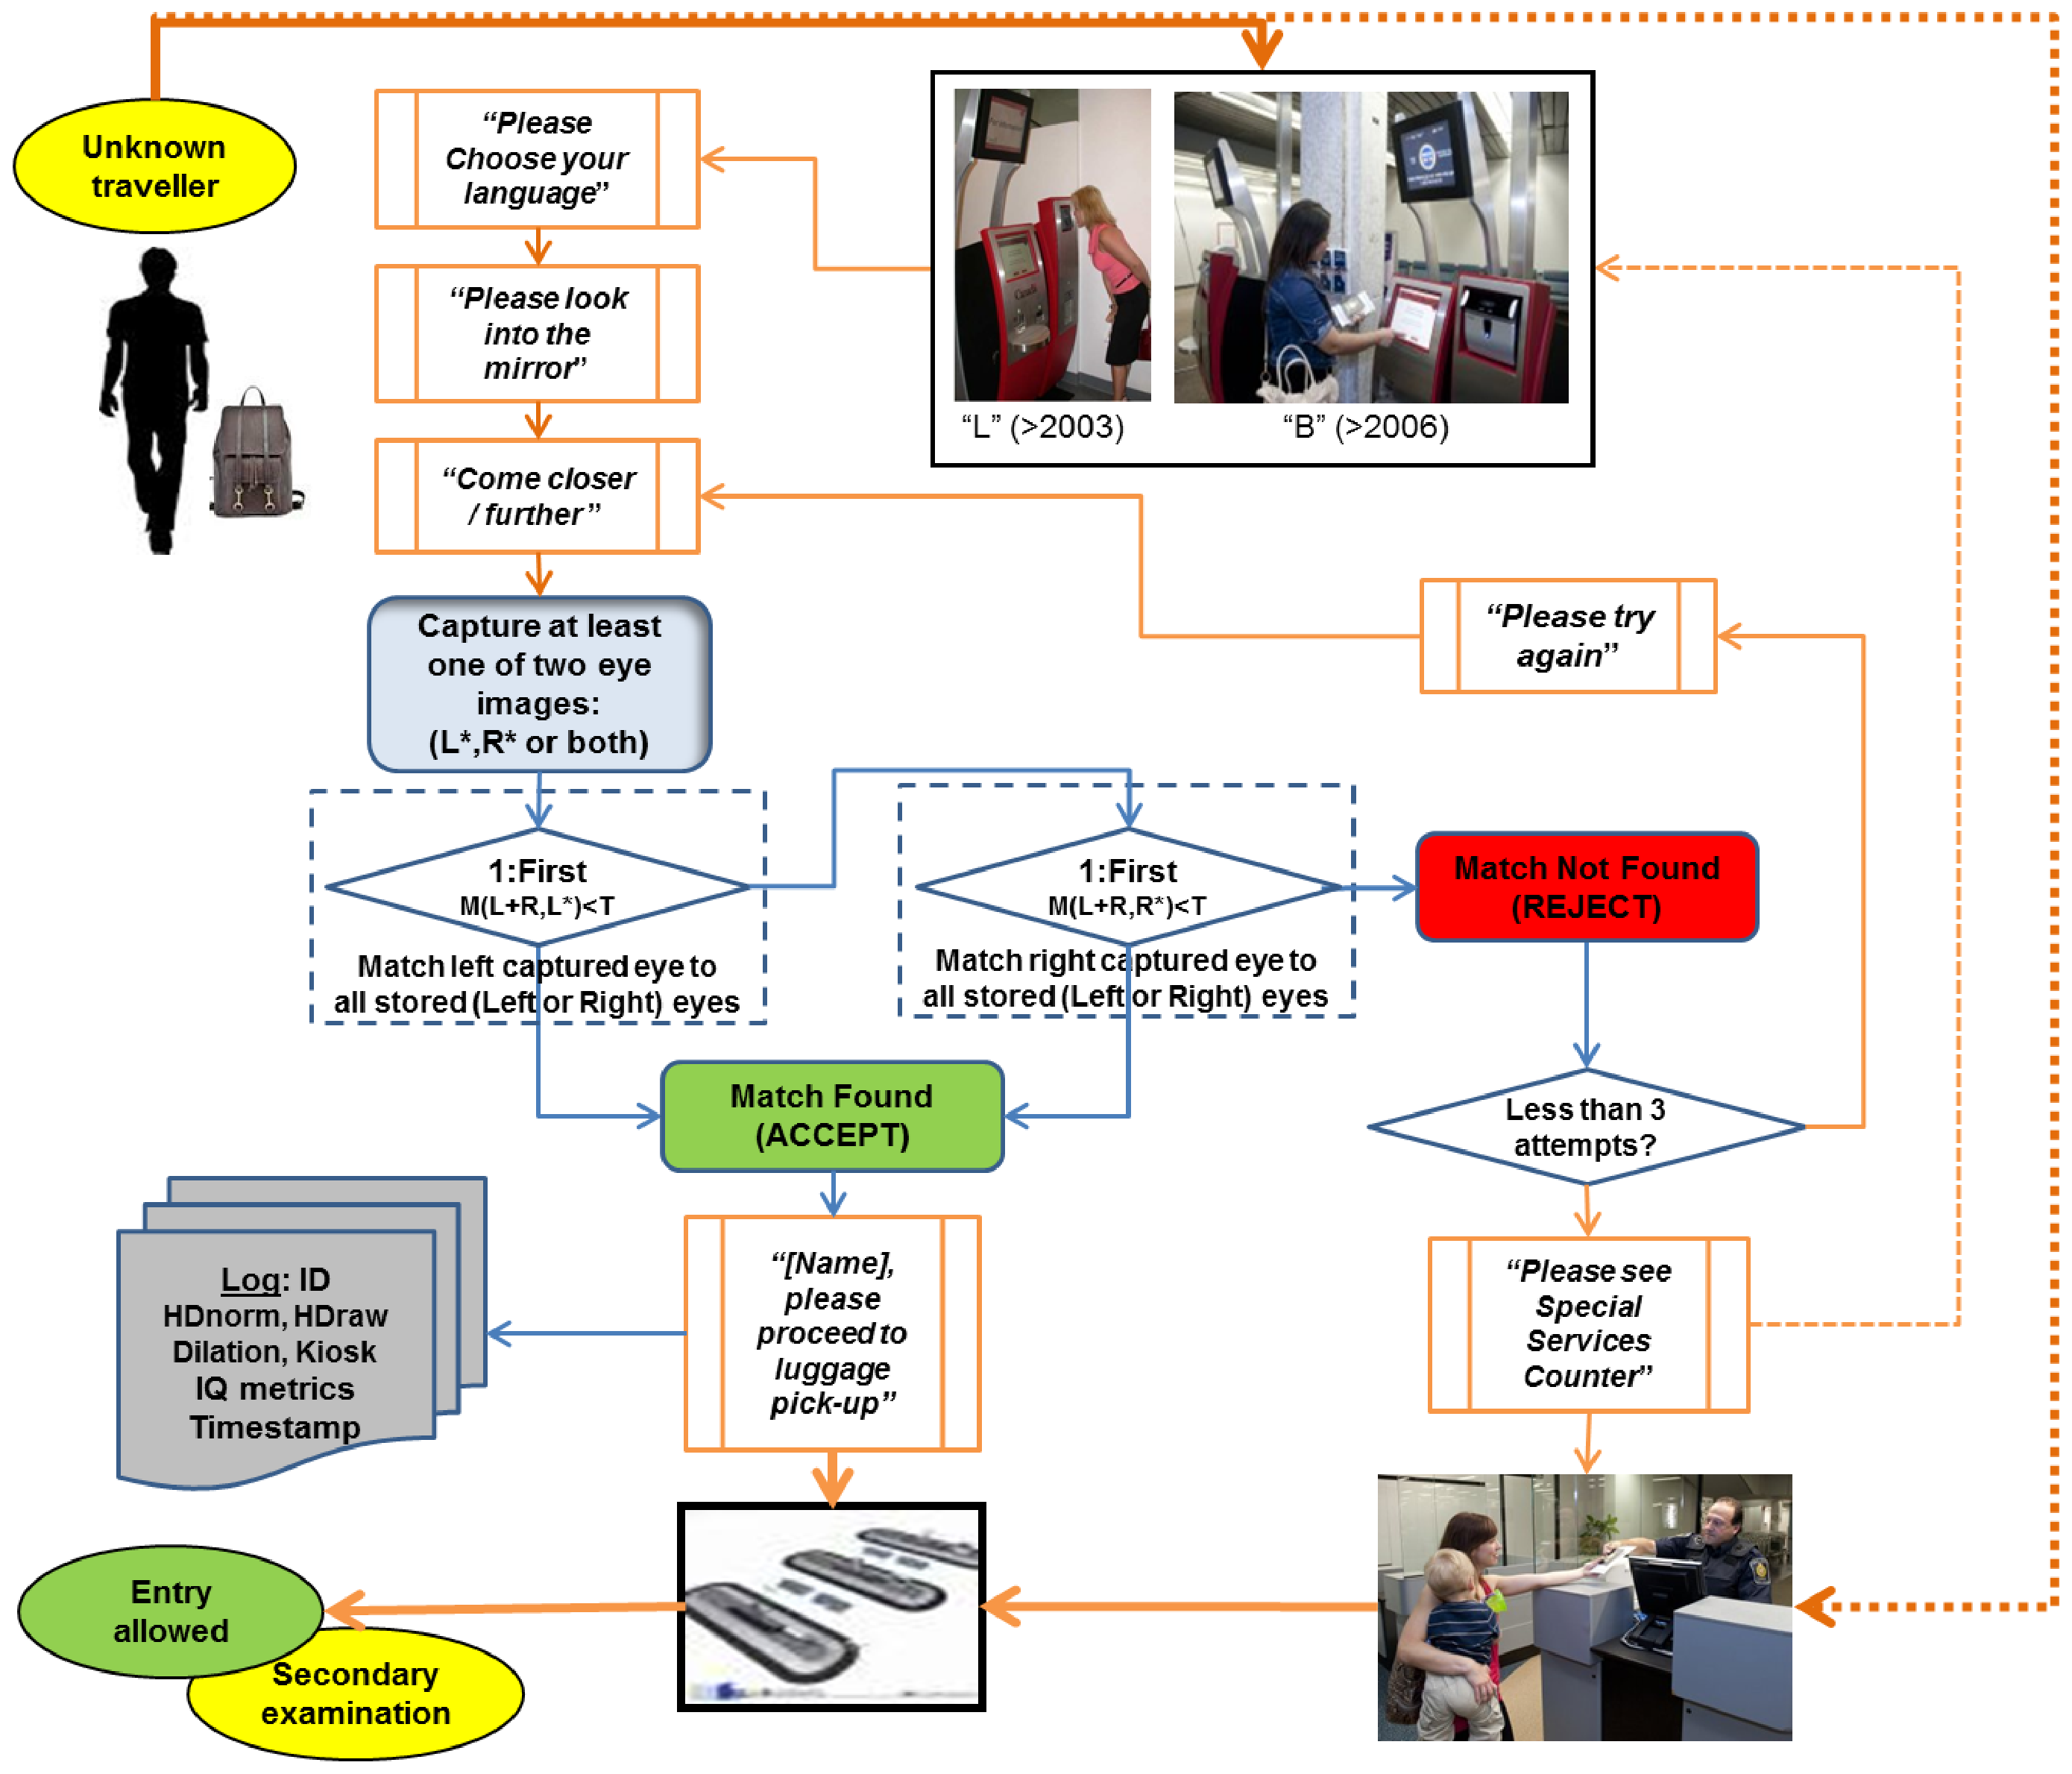
\includegraphics[width=14.5cm,height=12cm]{eps/nexus-workflow-new.eps} 
\caption{The workflow and decision logic of the NEXUS kiosks of the first generation, the log of which was used in NIST IREX IV iris aging study.  The system decision steps for match and rejection 
%for a person who has both eyes enrolled are 
are shown in dark blue arrows.  The user's procedural steps are shown in light orange arrows. Dashed orange arrows indicate optional steps for the users. 
%Only  the log of system steps is recorded. Users procedural steps are not known. 
\label{f.workflow}}
\end{figure*}


\section{NEXUS system description}
\label{s.description}

The CBSA commenced using iris recognition technology for automated authentication of travellers in airports in 2003, following the launch of a similar iris-enabled registered traveller program in the United Kingdom (UK). First,   it was used for CANPASS-Air \cite{[kn:CANPASS]}, which is a Canadian program that provides pre-enrolled pre-cleared Canadians expedited passage at arrival in airports for flights within Canada. Later in 2004 the use of iris-enabled identification of travellers was extended to the NEXUS-Air, which is a bi-national, Canada-US program for pre-approved low-risk travellers flying between Canada and the USA \cite{[CBSA-NEXUS]}. 

The expedited passage allows NEXUS members to proceed directly to the NEXUS self-serve kiosks, bypassing lengthy queues and interaction with customs border protection (CBP) officers and border services officers (BSO). 
%For each five-year NEXUS membership, the processing fee is Can\$50 or US\$50 per applicant. Children under the age of 18 are enrolled for free.
All kiosks are located in Canadian airports, owned and controlled by the CBSA, with iris biometric data being collected and stored by the CBSA. 
Kiosks used for travellers arriving to Canada are located in Primary Inspection Area.
%, in a special dedicated lane adjacent to manual Primary Inspection Lines (PIL). 
Kiosks used for travellers leaving Canada to the US are located in a special dedicated lane of the US pre-clearance area. 
In total, 69 NEXUS kiosks have been installed in Canada in eight Canadian airports: Calgary, Edmonton, Halifax, Montreal, Ottawa, two terminals at Toronto Pearson International Airport, Toronto Billy Bishop (Toronto City Airport), Vancouver and Winnipeg. Of these, 8 kiosks are used in Enrollment Centres and 22 kiosks are used at the US pre-clearance.
The same kiosks and iris database are used for both NEXUS-Air and CANPASS-Air programs. 
The number of CANPASS-Air users (about 2,000 people by 2014) however is significantly less than that of NEXUS-Air (over half a million in 2014).
%and is shrinking, because many CANPASS-Air members switch to NEXUS-air. 


%In contrast to the UK's IRIS program that has been dismantled after 10 years over the criticisms of its efficiency [2], the NEXUS program enjoyed a steady increase of its members over the years, with multiple blogs and reports praising its convenience and efficiency [2]. Most praised benefit of NEXUS membership for air travel is reported to be in expedited processing of transit travellers flying to the USA via Toronto or Vancouver airports, many of whom would have missed their connecting flights if not being a NEXUS member. A factor that limits use of the NEXUS program is reportedly the requirement that all accompanying family members must be NEXUS members [2].



Two designs (shown in Figure \ref{f.workflow}) 
were used for the NEXUS kiosks of the  first generation NEXUS system that were deployed from 2003 till 2014, the log of which comprises the OPS-XING dataset: with one-eye LG camera (deployed in 2003) and 
two-eye Panasonic camera (deployed in 2007). 

\cmt{
Three designs used for the NEXUS kiosks are shown in Figure \ref{f.kiosks}:  with one-eye LG camera (used from 2003 till 2007) and two-eye Panasonic camera (used from 2007 till 2014) 
%used in the first generation system, the log of which comprises the OPS-XING dataset,
and  with IrisID cameras installed in 2014 for the second generation systems that are presently deployed. 
%The notion of a  “generation'' in this context refers to two separate tender processes, rather than to two different technologies. 
The key difference of the second generation from the first generation is the use of the travel document to initiate 1-to-1 verification and the use of two different kiosk heights to better accommodate travellers of different heights.
%The first generation system used 1-to-First identification, which did not require a traveller to identify him/herself, but rather relied on the discriminatory power of the iris recognition technology, which at the time was believed to be sufficient to allow interaction-free retrieval of person’s identity from the list of all stored identities.
}




\subsection{System decision logic}

At the Enrollment stage, both irises of a traveller are photographed. Image Quality (IQ) control on iris images is performed. Only if their IQ metric is high, will they be enrolled into the system database. Because of image quality control, in some cases only one eye can be enrolled, and in some rare cases none of the eyes can be enrolled.
%, in which case a sticker is applied to the NEXUS card indicating that iris images are not captured. 
Travellers have also a choice of opting out from enrolling their iris images. %altogether, in which case the sticker is applied to their NEXUS card indicating that they have not enrolled the iris.
For travellers enrolling the iris, instructions are provided on how to use the kiosks, among which is the recommendation to remove eye-glasses and contact lenses of any type.  However, it is not known  how closely these recommendations are followed. 


%Figure \ref{} shows the frequency of enrollments per year and the percentage of them who could enroll one eye only.
%Figure \ref{} shows the frequency of enrollments per each age category and the percentage of them who could enroll one eye only. 
%From these figures it can already be seen that there are 



\cmt{
The workflow and the decision logic of the NEXUS kiosks of the first generation are summarized in 
Figure \ref{f.workflow}. 
}


At the time of crossing the border, referred to as the Passage stage, 
%At passage stage, 
the system is configured to search for the identity of the captured eyes using a 1-to-First search using the decision tree shown in 
 Figure~\ref{f.workflow}. 
Once the system captures person's eyes, it tries to authenticate a person using the Left eye only. If the Left eye is not matched, the Right eye is used. In both cases, the match is performed against all images (i.e., both left and right images) stored in the database  until the first image with a matching score below the threshold is found.
 %First, the system tries to authenticate a person using the Left eye only. If the Left eye is not matched, the Right eye is used. In both cases, the match is performed against all images (i.e. both left and right images) stored in the database  until the first image with a matching score below the threshold is found.
 This is due to the fact that first generation of NEXUS kiosks used single-eye iris cameras, which captured  an eye of person without knowing whether it was a left or right eye. 
%Later, such cameras were replaced with two-eye iris cameras (shown in Figure 0 1 b), however the system decision logic has remained unchanged because unknown number of previously enrolled irises may have been swapped.

%The decision to use 1-to-First, rather than 1-to-All matching commonly used in identification applications, is due to the original belief that iris modality does not allow more than one match. Later this has been proven to be not true, as some NEXUS members found that they were matched to someone else. The new generation of NEXUS kiosks, which are deployed now, do not have this issue, since they use 1-to-1 verification decision rule (i.e. matching a live image only to the image of the person whose name is on the NEXUS ID card.

When a traveller is rejected by the system (which happens because of one of two reasons: either IQ of live image is poor, or no matching image is found in the database), s/he is asked to try again, with the total of three  attempts  allowed in a single passage session with the kiosk. When a traveller is accepted, her/his attempt number at a given session is recorded.

A passage session ends either because of traveller's inactivity or the maximum number of capture attempts is reached, after which the system resets into the initial state with the ``Welcome. Please choose your language'' message.
Travellers who are not recognized  within a single session receive the ``Please visit Special Services Counter'' message. At the same time, they are also allowed to initiate additional passage session  using the same or different kiosks, which they can do as many times as they want. Similarly, they are also allowed to proceed to Special Services Counter any time they experience a problem with the kiosk. 

It is possible that some travellers, particularly those who experienced rejection problems in the past, have proceeded directly to the Special Services Counter  without  initiating a single session with the kiosks. 
There is no data left in the system log about these travellers.
The data from travellers who used the system but were rejected was also not logged.
This presents a critical limitation of the 
OPS-XING dataset made from historical NEXUS log data. By the design, this  dataset is biased towards better performing users, as it contains mainly the data from travellers who did not experience problems with the system and does not contain any rejected transactions.
Nevertheless, 
%being collected from the longest running border iris biometrics operation, 
even with this limitation, this dataset presents a unique and very valuable source for investigation of iris biometrics properties and limitations, specifically related to age and aging, which 
becomes particularly important now with iris modality becoming increasingly   used in many government and United Nations programs \cite{kn:Rathgeb-IBPC2014,FBI-IJCB2014} 
and the ongoing debate related to the tolerance of iris biometrics to aging \cite{IET0}-\cite{aging3}.





\begin{figure*}[!t]

a)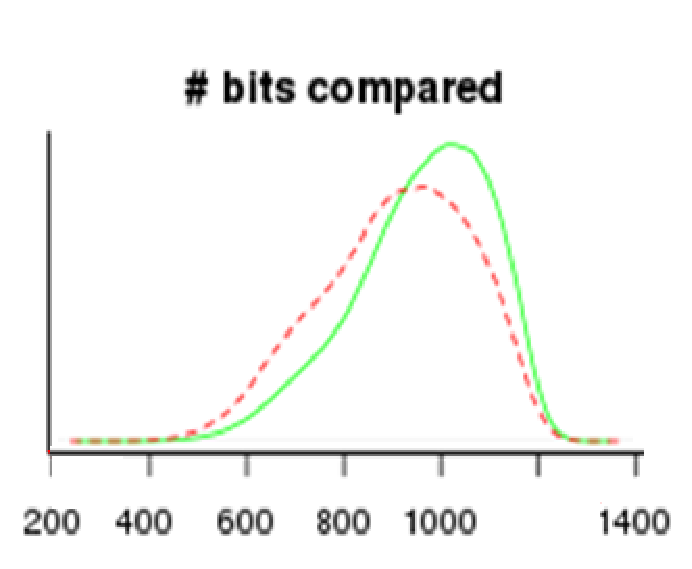
\includegraphics[width=0.15\linewidth,height=1in]{eps/bits-comp.eps}%
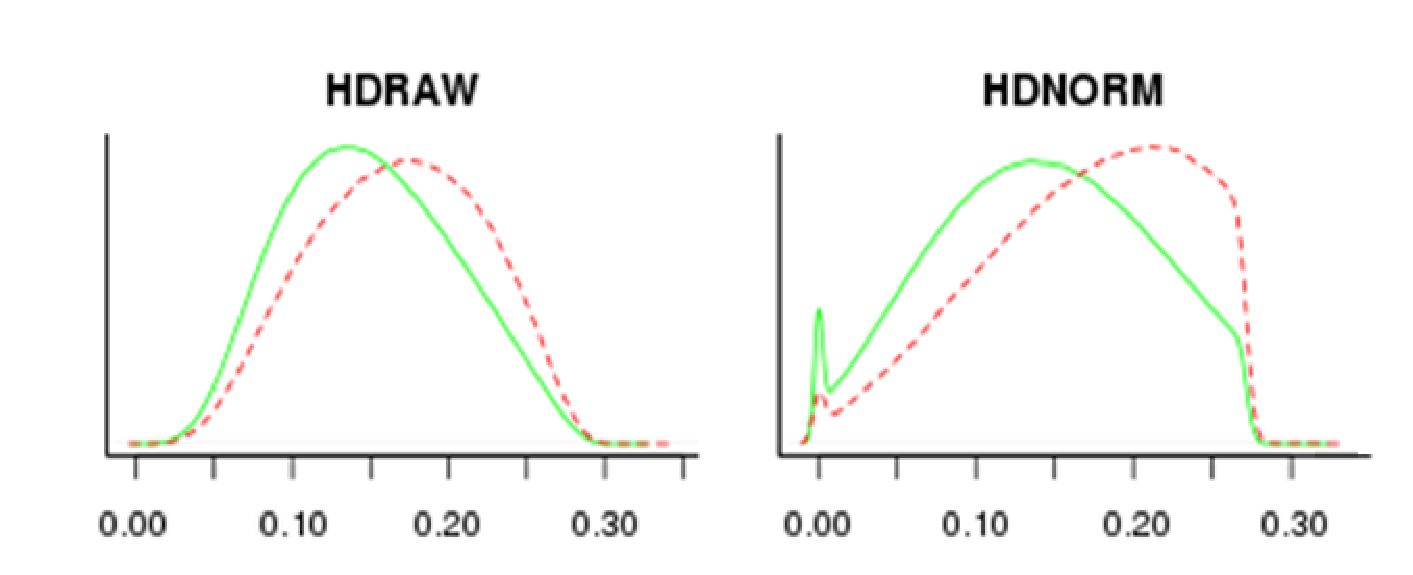
\includegraphics[width=0.335\linewidth,height=1in]{eps/HDnorm-vs-HDraw.eps} \quad 
%\vspace{5pt}\hrule\vspace{6pt}
b)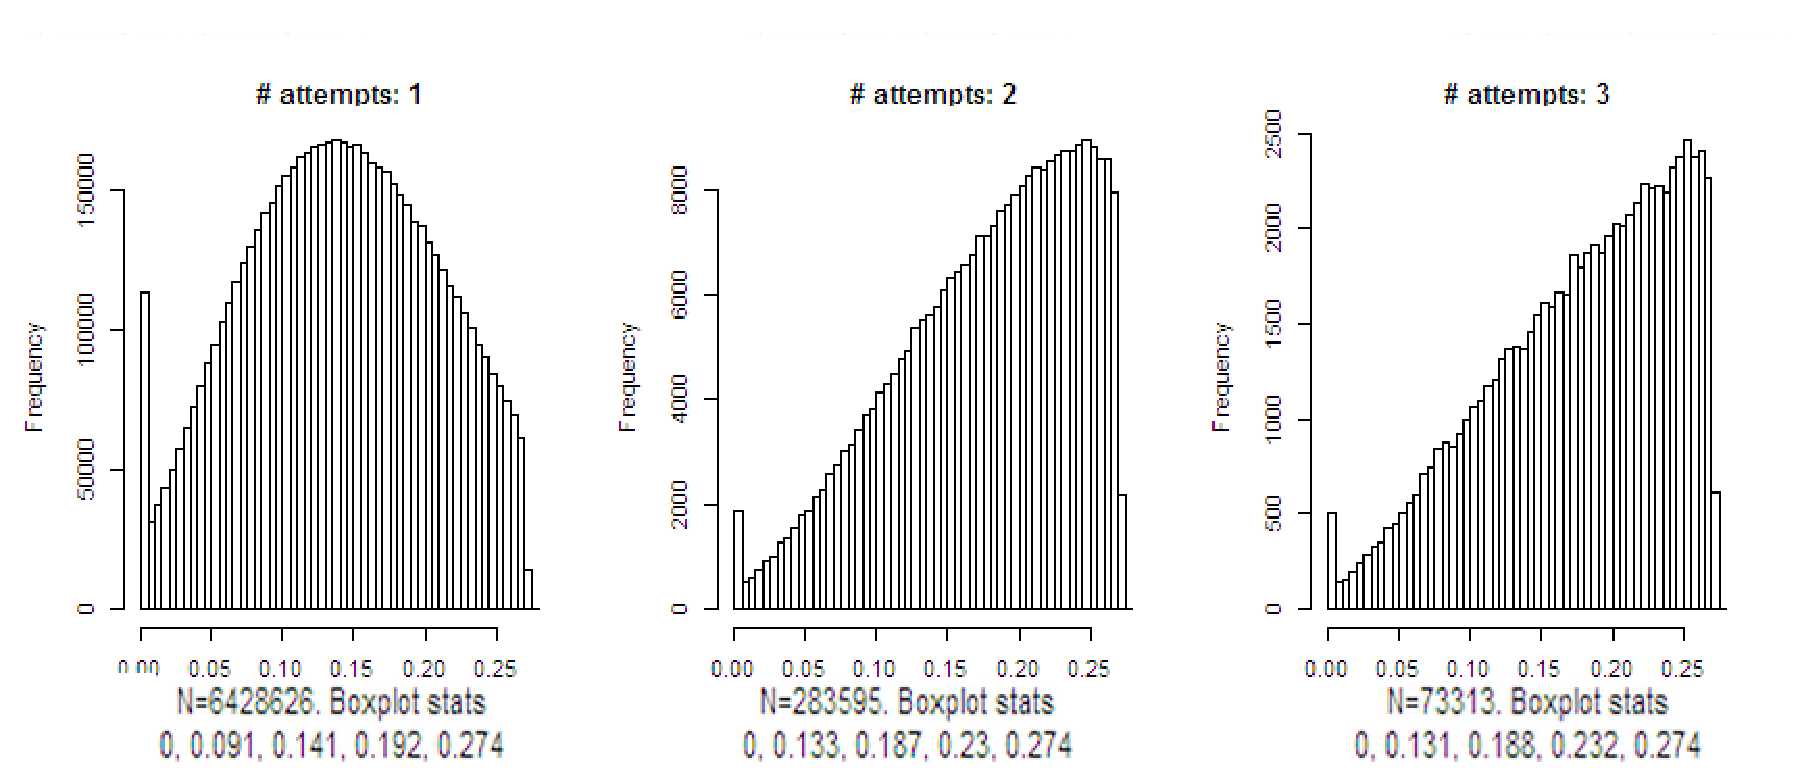
\includegraphics[width=0.5\linewidth,height=1in]{eps/HD=f(attempts)-c.eps} 
%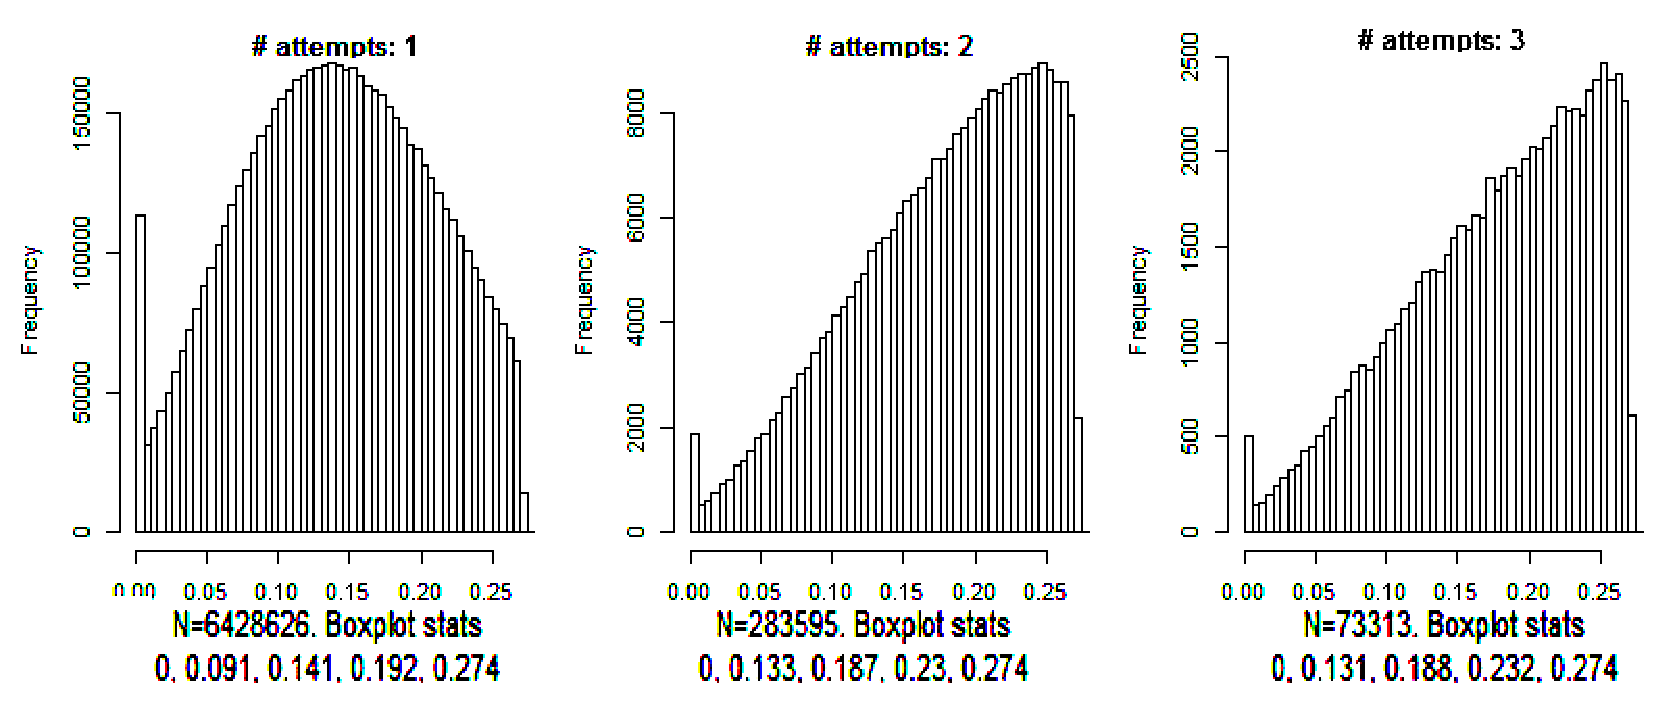
\includegraphics[width=0.5\linewidth,height=1in]{eps/HD=f(attempts)-c-best.eps} 

%\caption{Relative distribution of  Number of Bits Compared, HDNORM, HDRAW scores in the OPS-XING dataset 
%for left eye matches - in solid green, and for right eye  matches - in dashed red (top), and distribution of HDNORM scores for different number of attempts (bottom).
%}
\caption{Distribution of  Number of Bits Compared, HDRAW and HDNORM scores in the OPS-XING dataset. 
\figfooter{a} {  Left-eye scores (solid green) vs.   right eye (dashed red) scores; }
\figfooter{b} {Histograms of HDNORM scores for different number of attempts. 
%Observations: HDNORM distribution is not normal, HDNORM correlates with the number of attempts.
Minimum, 25\%, 50\%,  75\%, quartile and maximum values are shown at the bottom of each histogram.}
\label{fHDhisto}}
\end{figure*}


\begin{figure*}[!b]
\centering
%\centerline
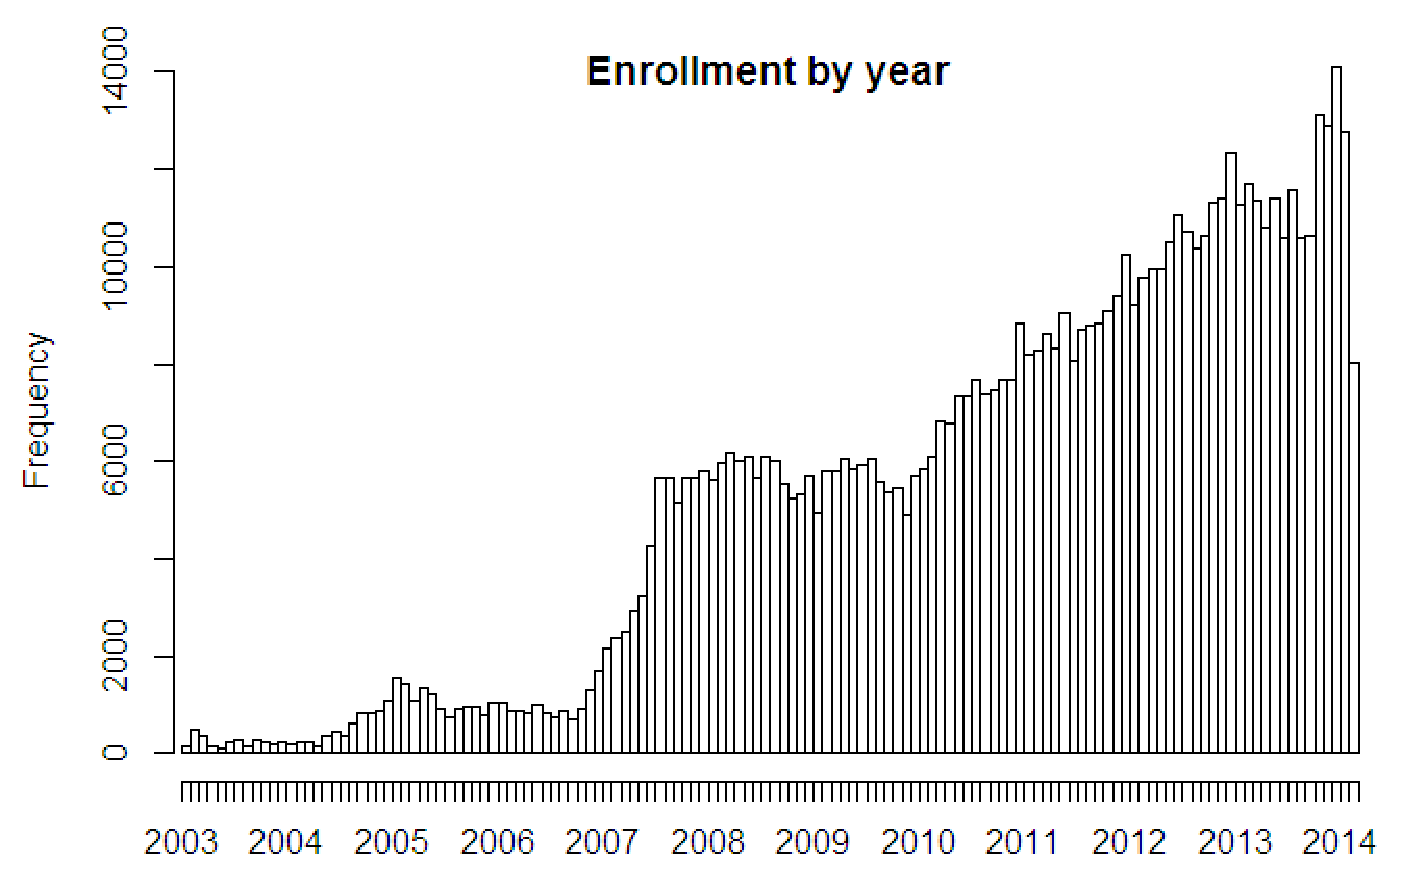
\includegraphics[height=1.5in, width=0.45\linewidth]{eps/en-by-year0.eps} \quad \quad \quad 
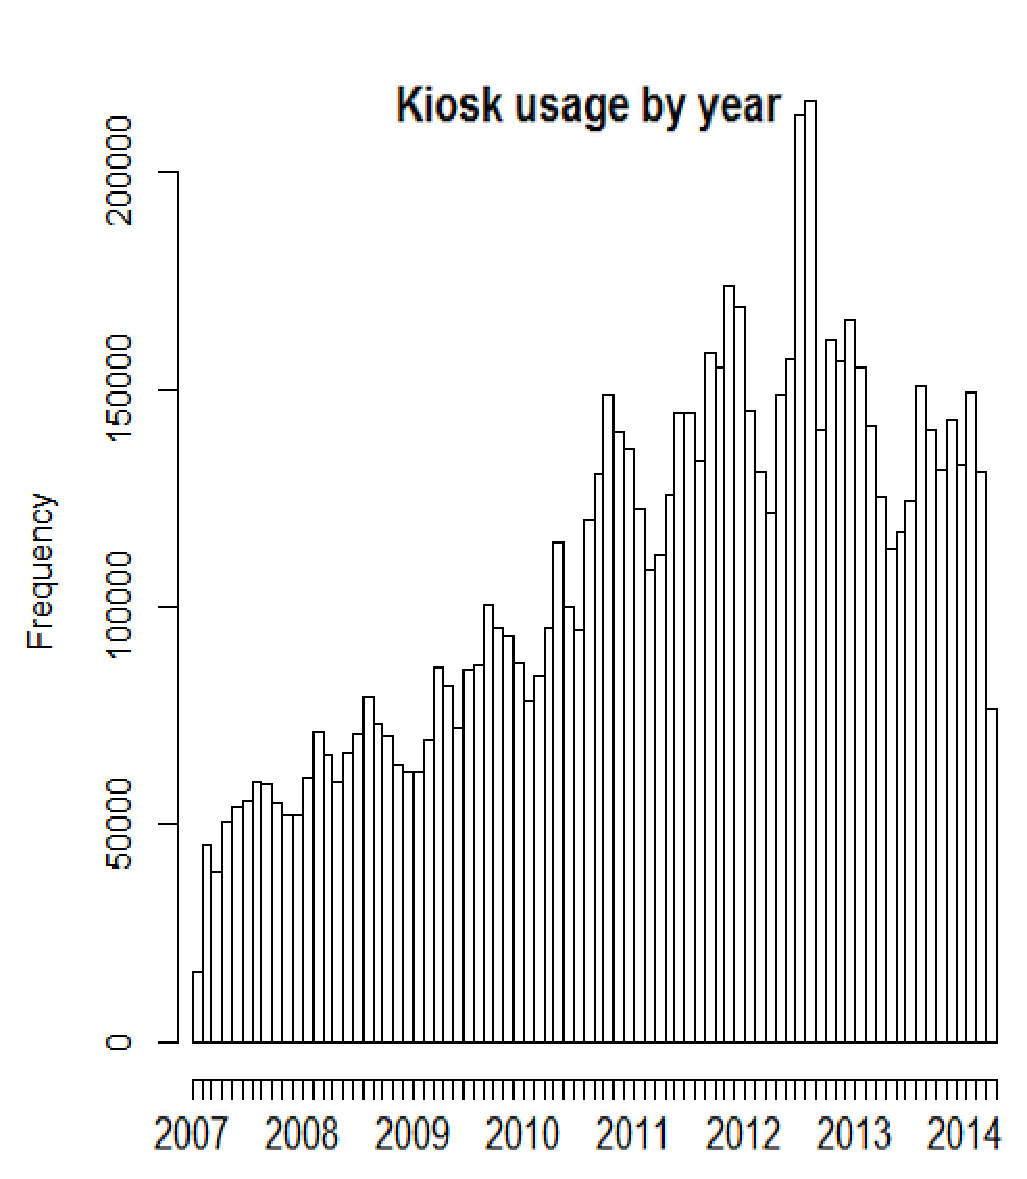
\includegraphics[height=1.5in, width=0.3\linewidth]{eps/pa-by-year0.eps} 

\caption{Number of  Enrollment  (left) and Passage (right) transactions    per month. %year.
}
\label{ftransactions}
\end{figure*}




\subsection{Iris recognition algorithm: %technology behind NEXUS kiosks}
Matching formula and threshold}
\label{s.NormRule}

NEXUS kiosks 
%of the first generation, from which the OPS-XING dataset is collected, 
use  Daugman's original iris recognition algorithm \cite{Daugman2002,Daugman2006}. The same version of the algorithm %(version 1.3.3) 
is used throughout the entire life-cycle of the system. 
c
%etc.
 %For example, iris boundary is no longer interpolated by a circle but rather by a set of ellipsoid curves. In a major improvement over the author's earlier algorithms, an equal number of masking bits are also now computed to signify whether  any iris region is obscured by eyelids, contains any eyelash occlusions, specular reflections, boundary artifacts of hard contact lenses, or has poor signal-to-noise ratio (SNR). 

%using only the real bits of the iris code, not the real and imaginary, as Daugman states in the paper discussed in the original review comments.

To our understanding, however, these later improvements of the algorithm are not implemented in the version that was used in the collection of the OPS-XING data.

Iris images are compared using the Hamming Distance ($HD$), which is a dissimilarity score between the corresponding  iris templates (IrisCodes). 
The score $HD=0$ means perfect match.  A high score (i.e., $HD >T_{HD}$) results in reject. The value of the threshold $T_{HD}$ is automatically selected by the algorithm based on the theoretical prediction of the False Accept Rate for a given number of entries in the data-base, slightly decreasing every year as the number of enrolled NEXUS members grew: from 0.282672 in 2006 (when the logging of the system commenced) to 0.271534 in 2014 (when the logging finished).

The Hamming Distance is computed in two steps.
% The $HD$ score is computed by compared two iris templates  (A) and (B)  to one another using  bit-wise comparison of the overlapping non-occluded bits from their IrisCodes ($bitsA$ and $bitsB$). 
First, the raw Hamming Distance $HDRAW$ is computed as the fraction of bits that disagree between two irises.
%, which is written in a simplified form as follows 
%$$HDRAW = bitsA {\rm XOR } bitsB, $$
%where XOR is the operator that computes the percentage of  unequal bits. 
%According to the theory established by the iris inventor, which assumes that computed bits are random independent variables, the average HDRAW between two random IrisCodes is 0.5 (or 50%).
%1.	Score normalization
Then, the normalized Hamming Distance $HDNORM$ is computed from $HDRAW$ following the normalization rule that gives less weight to comparisons performed on heavily occluded iris, using the following formula:
%, normalized Hamming Distance $HDnorm$ is computed from $HDraw$ following the normalization rule introduced by the algorithm  inventor  \cite{Daugman2006} :

\begin{equation}
HDNORM = 0.5-(0.5-HDRAW)\sqrt{  Nbits \over <Nbits>},  
\label{EQN}
\end{equation}
where ~~$Nbits$~~ is  the number of bits used in comparison  
%ranging from theoretical value of 2048 (when iris is not occluded, which never happens) or maximum observed value of to minimum obsrved value of 500.
%or less (when more than  three thirds of the iris is occluded),
and where~~
$<Nbits>$ is a vendor defined constant equal to 911, which, according to the original algorithm \cite{Daugman2006}, represents the average number of bits compared. 


Figure \ref{fHDhisto}-a  shows  $HDNORM$, $HDRAW$ and $Nbits$ score distributions in the OPS-XING dataset.
%The actual average value of $Nbits$ values of NEXUS kiosks, according to our results, is 954.
It is noted that, in contrast to   $HDNORM$ scores distributions, the $HDRAW$ scores distributions 
%do not have  artifacts 
have much less visible artifacts
due to score truncation and censoring, and are unimodal (i.e., have only one maximum). This makes analysis of  $HDRAW$ scores using statistical techniques easier.

%are close to normal, however the $HDNORM$ scores distributions are not. 
We also note that the actual average value of $Nbits$ is 954, which is higher than $<Nbits>$ constant used in the normalization formula (Eq. \ref{EQN}).


\subsubsection{Observation related to score normalization }
\label{s.score.normalization}

Through our analysis, the value of using the normalization step (\ref{EQN}) for the NEXUS application has been questioned in a number of ways. Besides producing non-unimodally distributed values (seen in Figure~\ref{fHDhisto}-a), which complicates modeling the system performance using statistical methods, it also contributes to higher false reject rates for travellers with  occluded iris.

A number of ways are seen to further improve the matching formula for the application. This includes post-processing score normalization described in \cite{GorodnichyScore},  the use of conditional normalization formula (conditioned on additional image quality metrics such as contrast and/or person's age), which are analyzed further in the paper, or not applying the normalization formula (Eq. \ref{EQN}) at all. These however are outside of the scope of this paper. 

In this paper  it is the importance of analyzing $HDRAW$ in combination with image quality metrics, as opposed to analyzing  $HDNORM$ scores only as done in the past, that is emphasized. 


\subsubsection{Observation related to the correlation between matching score and number of attempts }
\label{s.HDvsAttm}

%Figure~\ref{fHDhisto} shows the distribution of matching scores for different number of attempts. The five-number statistics   (minimum, 25\%, 50\%,  75\% quantiles, maximum) are also shown there. It is seen that the larger the number of attempts, the larger the matching scores, confirming the results presented in \cite{Bowyer-attempts}. In our analysis, the number of attempts is used along with matching scores $HDRAW$ and $HDNORM$ as one of the kiosk performance metrics. 

In our analysis, in addition to the matching score ($HDRAW$ and $HDNORM$), we also use the number of recorded attempts ($\# Attempts$) as one of the important kiosk performance metrics. 
There exists a subtle relationship between the two,  illustrated in Figure~\ref{fHDhisto}, which  
shows the distribution of matching scores for different number of attempts and the corresponding five-number statistics for $HDNORM$.%: its minimum, 25\%, 50\%,  75\% quartiles, and maximum values).
%however they are not the exact dirivative of one another.

On one hand, it is seen that the larger the number of attempts, the larger the matching scores, as reported in \cite{Bowyer-attempts}.
On the other hand, a higher matching score does not necessarily mean that a person gets rejected (as long as the matching score is less than the threshold, a person is accepted). Similarly, recognition from a single attempt does not necessarily mean that a person has not tried and was already rejected multiple times during other sessions that were not logged. 
Therefore, using both metrics in the analysis  provides richer complementary evidence for the results obtained.



\begin{table*}[!t]
	\caption{Metrics recorded in the OPS-XING dataset. 	
	\label{MetricsRecordedAtOPSXINGDataSet}}


\begin{small}

		\begin{tabular} { l | l }
		\hline
			At Enrollment & 
			\textbf{FAKE\_ID}, age, %gender, 
\textbf{EYE} (L-left or R-right), 
\textbf{CAMERA }(`L' for old LG camera, `B' for new Panasonic camera) \\ 
& ENROLLMENT\_DATE (month, \textbf{year}, time of the day)
\\ 
& IQ metrics:  related to localization accuracy --- 
			iris center x,   iris center y; 			 iris radius; 	pupil center x,  pupil center y; 
			\\ 			& 
\quad related to dilation ---  
pupil radius,   
pupil iris ratio  (the same as \textbf{DILATION});		
			\\ 			& 		
\quad related to image contrast --- 
iris sclera contrast,
	iris pupil contrast, 
	average iris intensity, 
	iris texture energy;    
			\\ 			& 
\quad related to  occlusion --- 
iris area,     
	number of bits encoded   
\\ \hline
				At Passage & 
				\textbf{FAKE\_ID},
\textbf{EYE used},
TRANSACTION\_DATE (\textbf{month}, \textbf{year}, time of the day) \\ 			& 
\textbf{ELAPSED\_TIME} (the number of days since enrollment) 
\textbf{HDNORM}, HDRAW 
		\\ 			& 
\textbf{CAPTURE\_NUMBER\_WITHIN\_PA} (capture-and-recognize attempts)
			\\ 			& 
\textbf{FAKE\_KIOSK\_ID,}
\textbf{THD} (matching threshold), 	
\textbf{MATCHING\_MODE} (SEP: two-eye pilot, SEM: regular one-eye operation), 
							\\ 			& 
				IQ metrics: same as at Enrollment,
				number of bits encoded, number of bits compared 
				\\	
				\hline
		\end{tabular}

{\footnotesize
Note: metrics used in the previous work \cite{irexVI}-\cite{Bowyer-BTAS2016} are marked bold.
% monthly frequencies  of  enrollment and passage transactions   per month are shown in Figure \ref{ftransactions}. 
The distributions of metric  values are shown in  Figure \ref{fCorrelationAgeIQ}.
}

	\end{small}
\end{table*}




\begin{table*}[!b]
\processtable{Number of travellers as the function of the number of times they used the system and  percentage among them experiencing ``difficulty''.\label{fNumberBAd}}
{

{\footnotesize 	
\begin{tabular}{|l|c|c|c|c|c|c|c|}
\hline
Times used the system & 2+ & 4+ & 8+ & 16+ & 32+ & 64+ & 128+\\
\hline
Number of travellers & 383,463 & 287,472 & 196,573 & 119,538 & 61,332 & 24,383 & 6,530\\
\hline
Percentage of them having $HDNORM>0.2$   & 4.2\% & 2.4\% & 1.3\% & 0.8\% & 0.6\% & 0.3\% & 0.2\%\\
Percentage of them having $Attempts>1.5$ & 3.4\% & 2.4\% & 1.3\% & 0.6\% & 0.3\% & 0.12\% & 0.06\%\\
\hline
\end{tabular}
}

}{}


{\footnotesize Note: 
%The ``difficulty'' is measured in terms of high minimum HD score ($HDNORM>0.2$). 
%The table shows the number of travellers who  used the system more than 2, 4, 8, 16, 32, 64 and 128 times, and the percentage among them who experienced ``difficulty'', where ``difficulty'' is measured in terms of high minimum HD score ($HDNORM>0.2$). 
%Table show the number of travellers who used the system at least once  (everyone) to over 128 times (1\% of travellers). Right plot shows the percentage among them who experienced ``difficulty''. 
``Difficulty'' is measured by high minimum HD score ($HDNORM>0.2$)  and high average number of attempts ($Attempts > 1.5$). 
The temporal information (i.e., whether a traveller used the system over a short or long period of time) is not used.
More details are provided in \cite{GorodnichyARTinABC}.
}

\end{table*}



\section{OPS-XING dataset}
\label{sOPSXING}

The OPS-XING dataset,  a part of which was used in the IREX VI evaluation by NIST \cite{irexVI,Grother2015-iet} and the evaluations conducted by UND \cite{Bowyer2015-iet,Bowyer2015-cvpr,Bowyer-BTAS2016},
%was collected from the ``first generation'' NEXUS kiosks and 
consists of over a quarter billion  of 
%scores and   metrics  that were recorded by the NEXUS system, which are listed in Table \ref{MetricsRecordedAtOPSXINGDataSet}.
matching and image quality metrics that were recorded during Enrollment and Passage transactions
by the NEXUS system. 
These metrics are listed in the Table~\ref{MetricsRecordedAtOPSXINGDataSet}.
The  metrics that were shared with NIST and UND and used in previous research \cite{irexVI}-\cite{Bowyer-BTAS2016} are marked bold.


%in its enrollment and passage transactions. 
In total, there were 1,370,890 enrollment transactions (recorded from September 2003 till May 2014,
from 
%702,526 
705,553
travellers --  
most  (662,220)  done with dual-eye Panasonic cameras deployed in 2007, others done by single-eye LG  cameras) 
%43,338, mostly prior to June 200  with single-eye LG (`L') cameras and 662,220  with new dual-eye Panasonic (`B') cameras), 
% using old and new camera, 
and over 10 million passage transactions (recorded from October 2007 till May 2014, from 467,314 travellers  -- 
all done with dual-eye Panasonic cameras).
\cmt{
Enrollment images prior to June 2007 are all captured using single-eye LG (`L') cameras. After June 2007, most of them are captured using new Panasonic cameras, some however were still captured by old LG cameras.
%occasionally old LG camera was also used up till 2014. 
All passage images in the dataset are captured using new Panasonic cameras.  
% The number subjects who with left eye only, right eye only and both eye enrollments is shown in  Table \ref{}. The table also shows the number of left eye and right eye transactions at passage.
}
Distribution of Enrollment and Passage transactions over the years is shown in Figure \ref{ftransactions}. Seasonal patterns in Passage data can be noticed.
\cmt{
In total,
1,370,890 enrollment transactions from 2003 till 2014
from 
%702,526 
705,553
travellers were recorded, of which 43,338 were enrolled with 'L' camera... ,  
and over 10 million passage transactions were recorded 
466,070 travellers
from October 2007 till May 2014 from 467,314 travellers (see Figure \ref{ftransactions}).

}

\cmt{
%The metrics that were recorded in enrollment transactions are the following: 
person's FAKE ID, gender, age at the time of enrollment, enrollment date (month, year, time of the day), \textbf{eye enrolled} - left or light,  \textbf{camera used} - LG (''L'') or Panasonic(``B'') and 
fourteen image quality scores, including pupil dilation score which was used in the studies conducted by NIST and UND 
%shown in Figure \ref{}
%of which only dilation is considered in the  analysis presented in this paper
%Other IQ scores have been also analyzed in our 

%, defined as a pupil to iris radii ratio 
}

\subsection{Aberrations in data}


The OPS-XING dataset contains a number of abnormal entries that are not described by the system logic. 
%Special effort of the conducted analysis was given to detecting and explaining the aberrations in the OPS-XING data. 
Mostly caused by human error or temporal experimentation with the system (either by kiosk users or programmers), such aberrations in data may give rise to additional challenges in understanding the technology and arriving to the correct conclusions by  external researchers who  process this historical dataset. These data aberrations are described below. 
They needed to be removed or taken into account  prior to conducting the analysis. 
%not  to introduce spurious 
%so that not to introduce noise into data analysis
%not to give rise to false results

\textbf{HD scores higher than threshold:} There are 351 passage transactions in two Kiosks 
%(OK18 and OK34) 
that happened with Right eye  which have $HDNORM > THD$. These are from the Pilot  that was conducted in 2012, in which the first eye is recognized but the second eye is verified as 1:1. 
%The pilot was run for two months  and then it was closed because it did not catch false matches.

\textbf{More than three  attempts:} There are 1495 passage events in which there were more than three  attempts.
% ($CAPTURE\_NUMBER\_WITHIN\_PA >3$). 
These are due to  some users unexpectedly interrupting the operation of the kiosk in the middle of its operation.

\textbf{Enrollments of left and right eye on different days}: Some 
(14) 
travellers have eyes enrolled on different years.  When there was a problem enrolling an eye image, the older eye image was often kept.

\textbf{Multiple enrollments (dilation scores) at enrollment:} Some 
(1405) 
travellers have multiple IQ data (including dilation score) at enrollment transactions for the same eye, due to applying several attempts to enroll the iris.

%at entothere are data has more lines than EN data. Only those that have the same DILATION in both EN and ENIQ are left for analysis. However some EN had the same DILATION with multiple lines in ENIQ. In these cases, the first match was used. Other lines were removed from the analysis. 

\textbf{Other issues}:  
As mentioned above, the system performs a 1-to-First search. In doing that a new probe iris image, which can be either from  Left eye (default eye) or Right eye (when Left eye did not find the match) is compared to \textit{all} iris images stored in the enrollment database, including left and right eye images, and sometimes old and new name-records of a person.  
%Theoretically, this could have resulted in increased number of false zero-effort non-matches, which could be present in the dataset and which could not be detected. 
This results in some unknown number of zero-effort false match scores being recorded as part of the dataset.


%\subsection{Upgraded version of OPS-XING dataset} %Filtered dataset} %


%have been filtered out from the OPS-XING dataset as outliers and are described below. More details are provided in Appendix C. 
A  filtered  version of that OPS-XING  dataset with
data aberrations marked or removed has been prepared and used in our analysis.

%To facilitate further analysis, the dataset set is divided into three main data-tables:  containing information about system users (dUsers), Enrollment and Passages
%The descriptive statistics of their key fields is presented below.

%, referred to as Release 4.1.0, ready for further scientific analysis.

%In this paper, we focus on the analysis of the effect of AGE variable on the performance of the system.
%, where the performance is measured in term av
%The analysis of other variables is presented elsewhere \cite{2016-DG-ieee}



\begin{figure*}[!t]
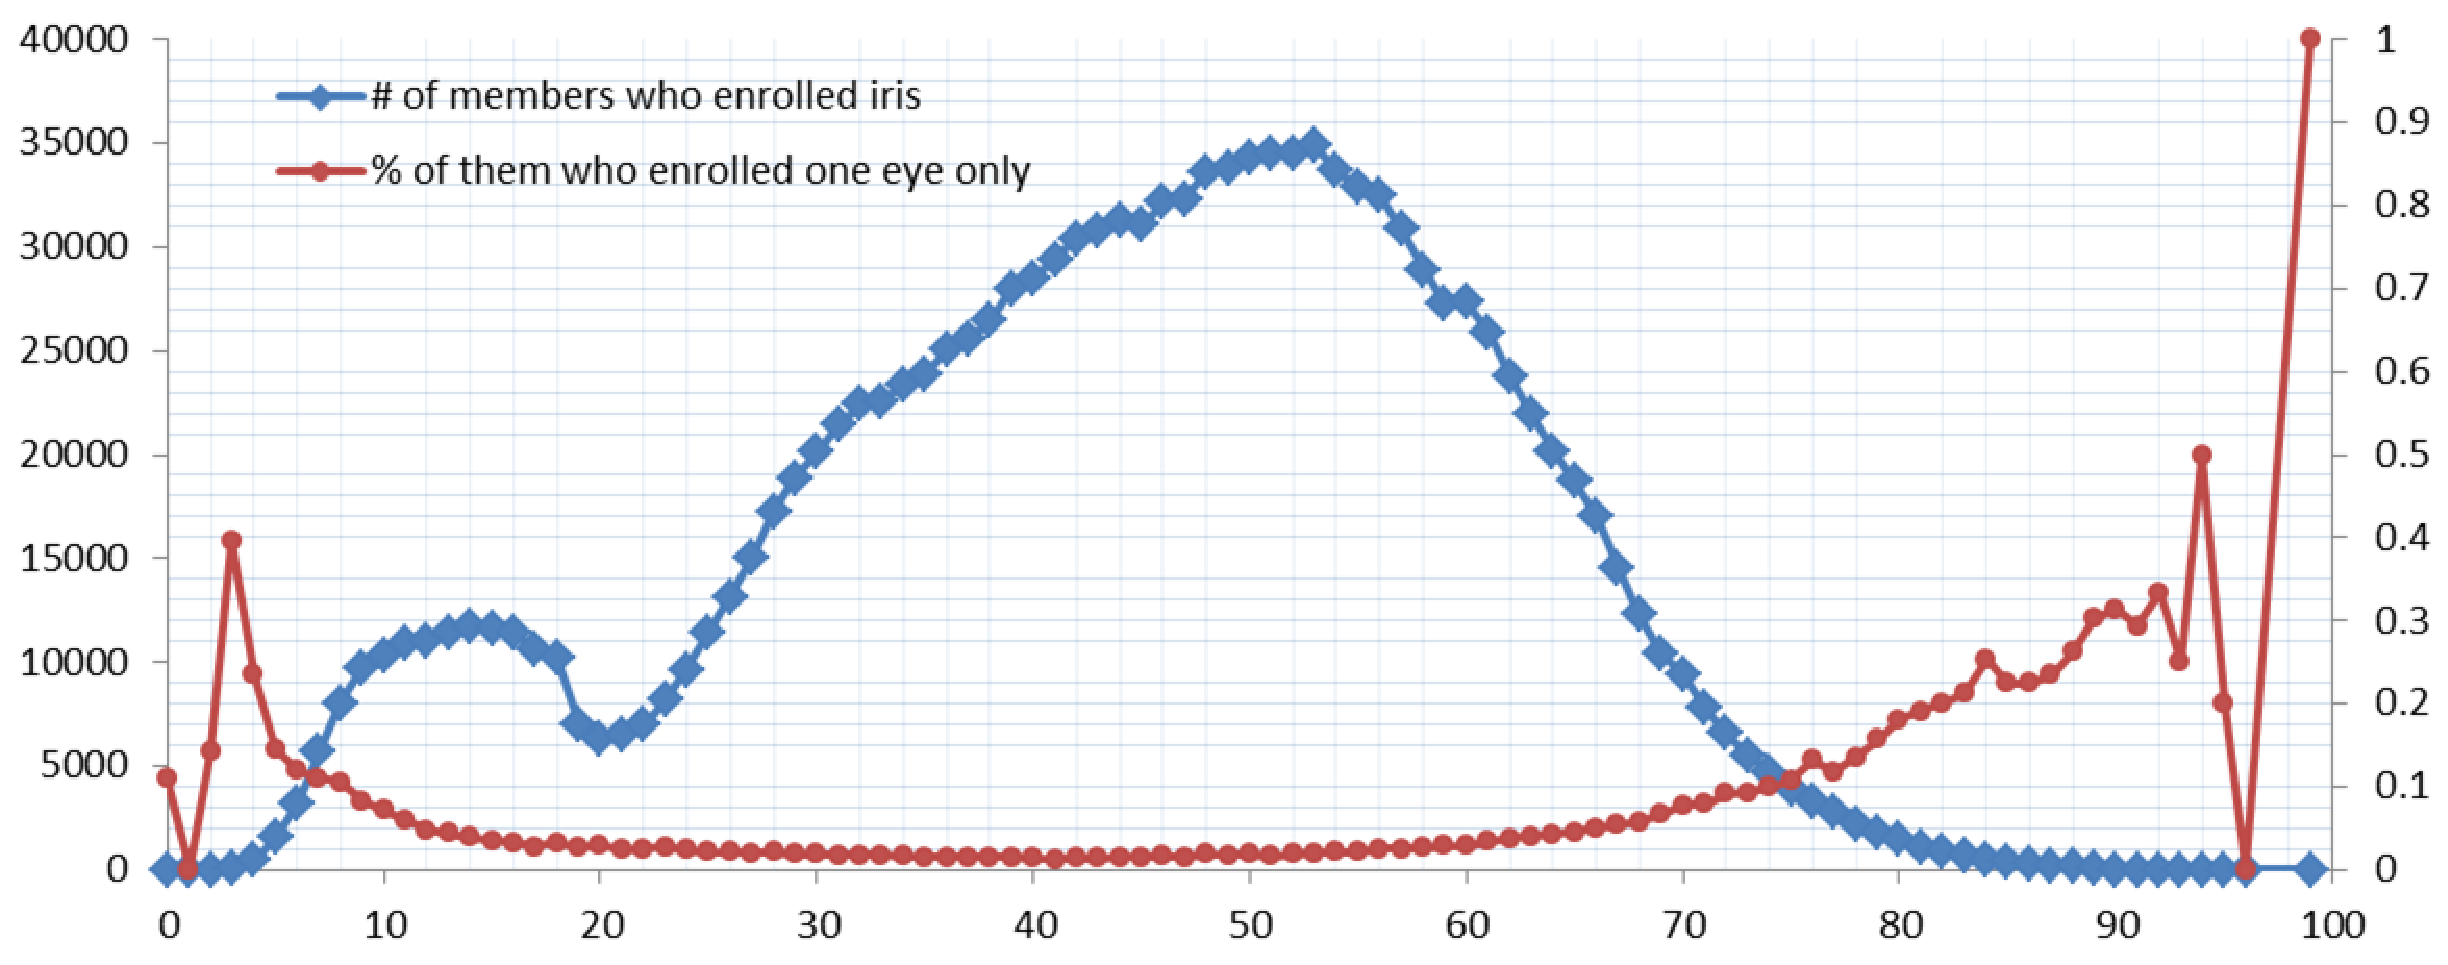
\includegraphics[width=0.45\linewidth,height=1.4in]{eps/age-one-eye.eps}\quad 
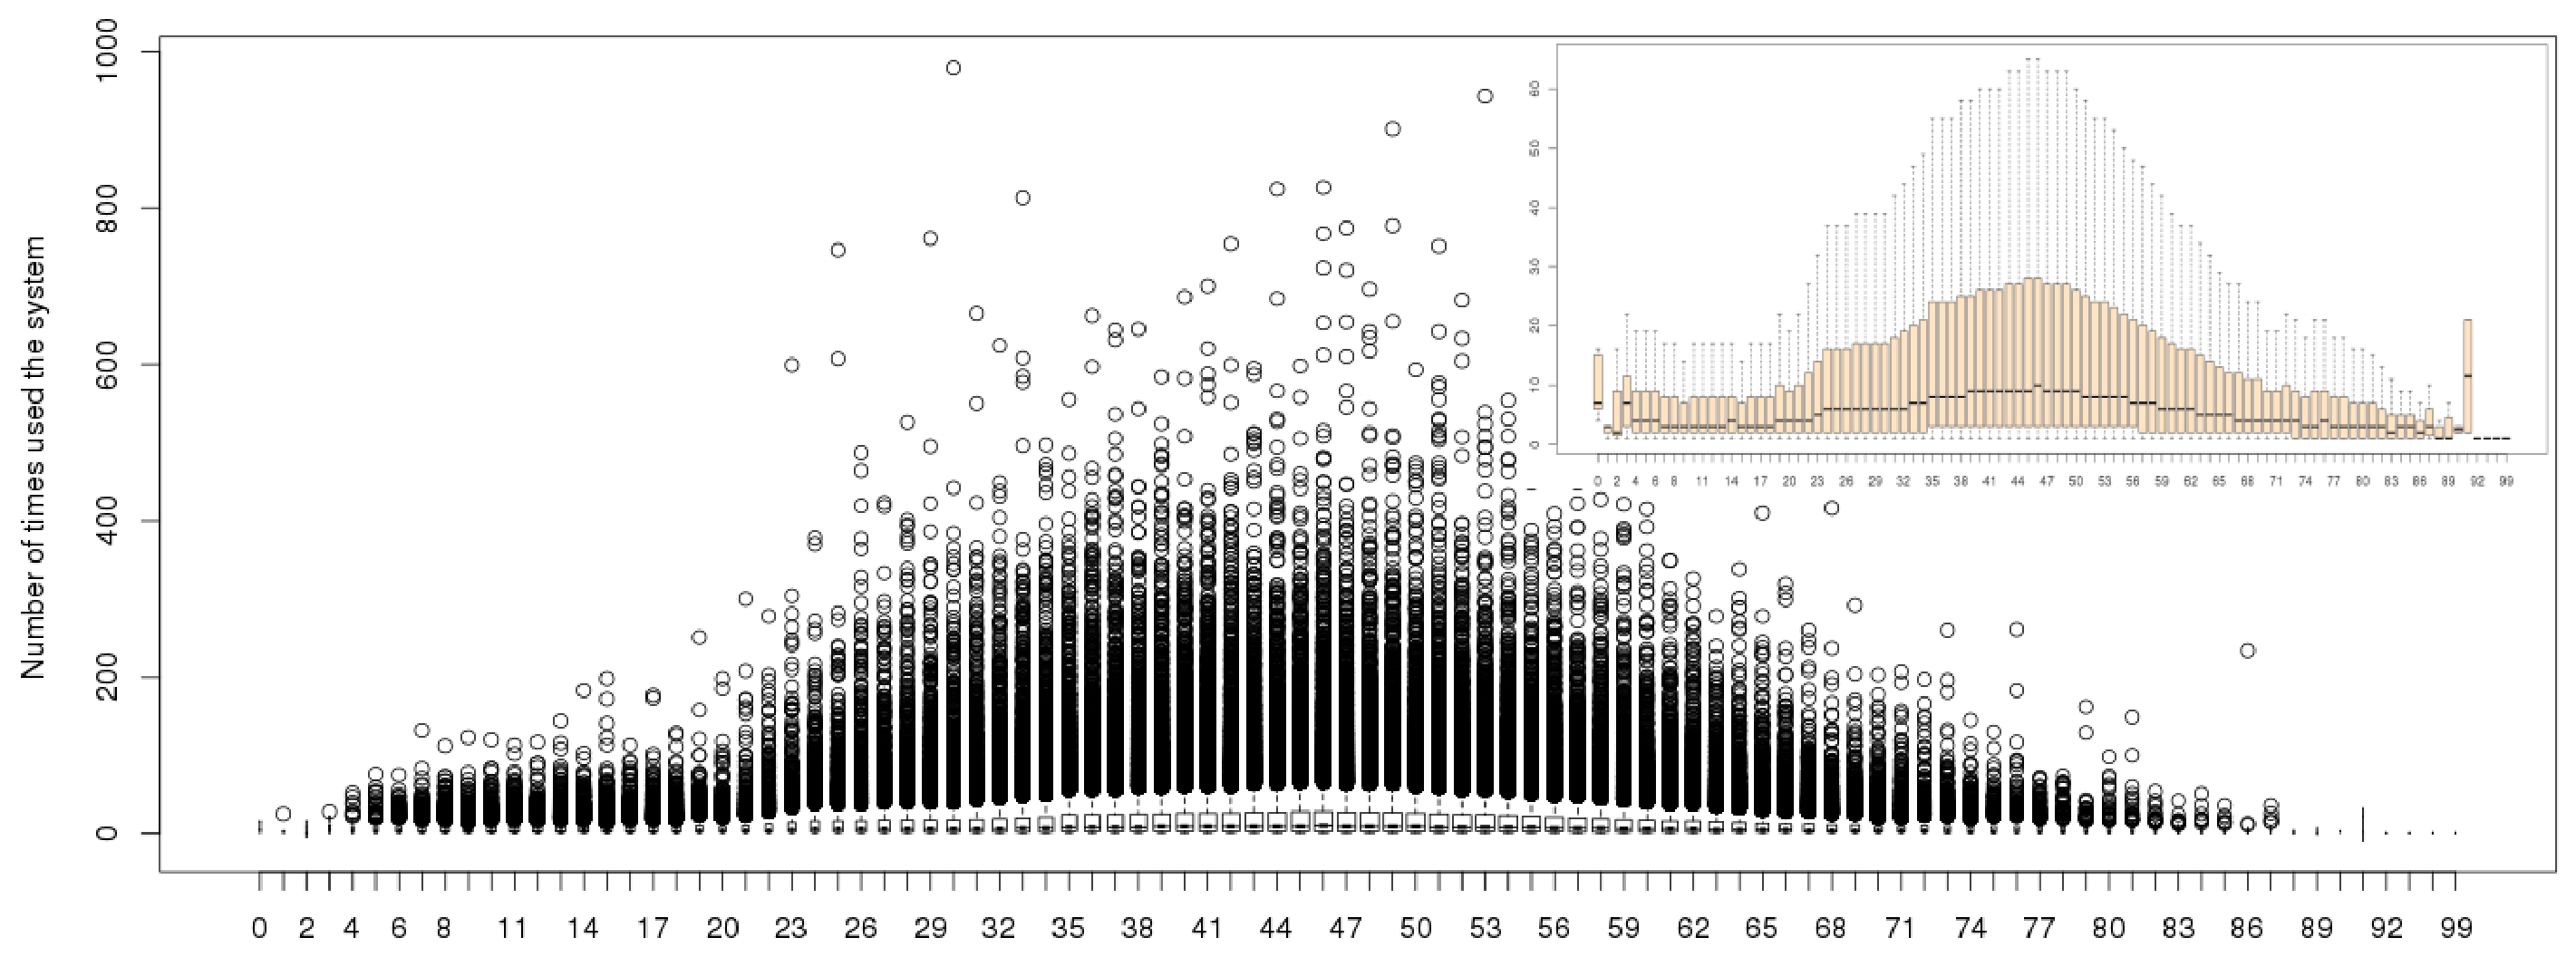
\includegraphics[width=0.55\linewidth,height=1.4in]{eps/USED-wInset-0.eps} 
%\includegraphics[width=\linewidth,height=1in]{eps/USED-by-AGE.eps}

\caption{
The number of travellers by age at Enrollment and Passage. 
Left image shows the number of travellers who enrolled iris (in blue) and the percentage among them who were able to enroll one iris  only (in red). 
The right image shows  boxplots summarizing the number of passages for each age. Inset shows 95\% truncated boxplots (i.e., with 5\% of outliers removed). 
}
\label{fBoxplot-IQen}
\end{figure*}


\begin{figure*}[!b]

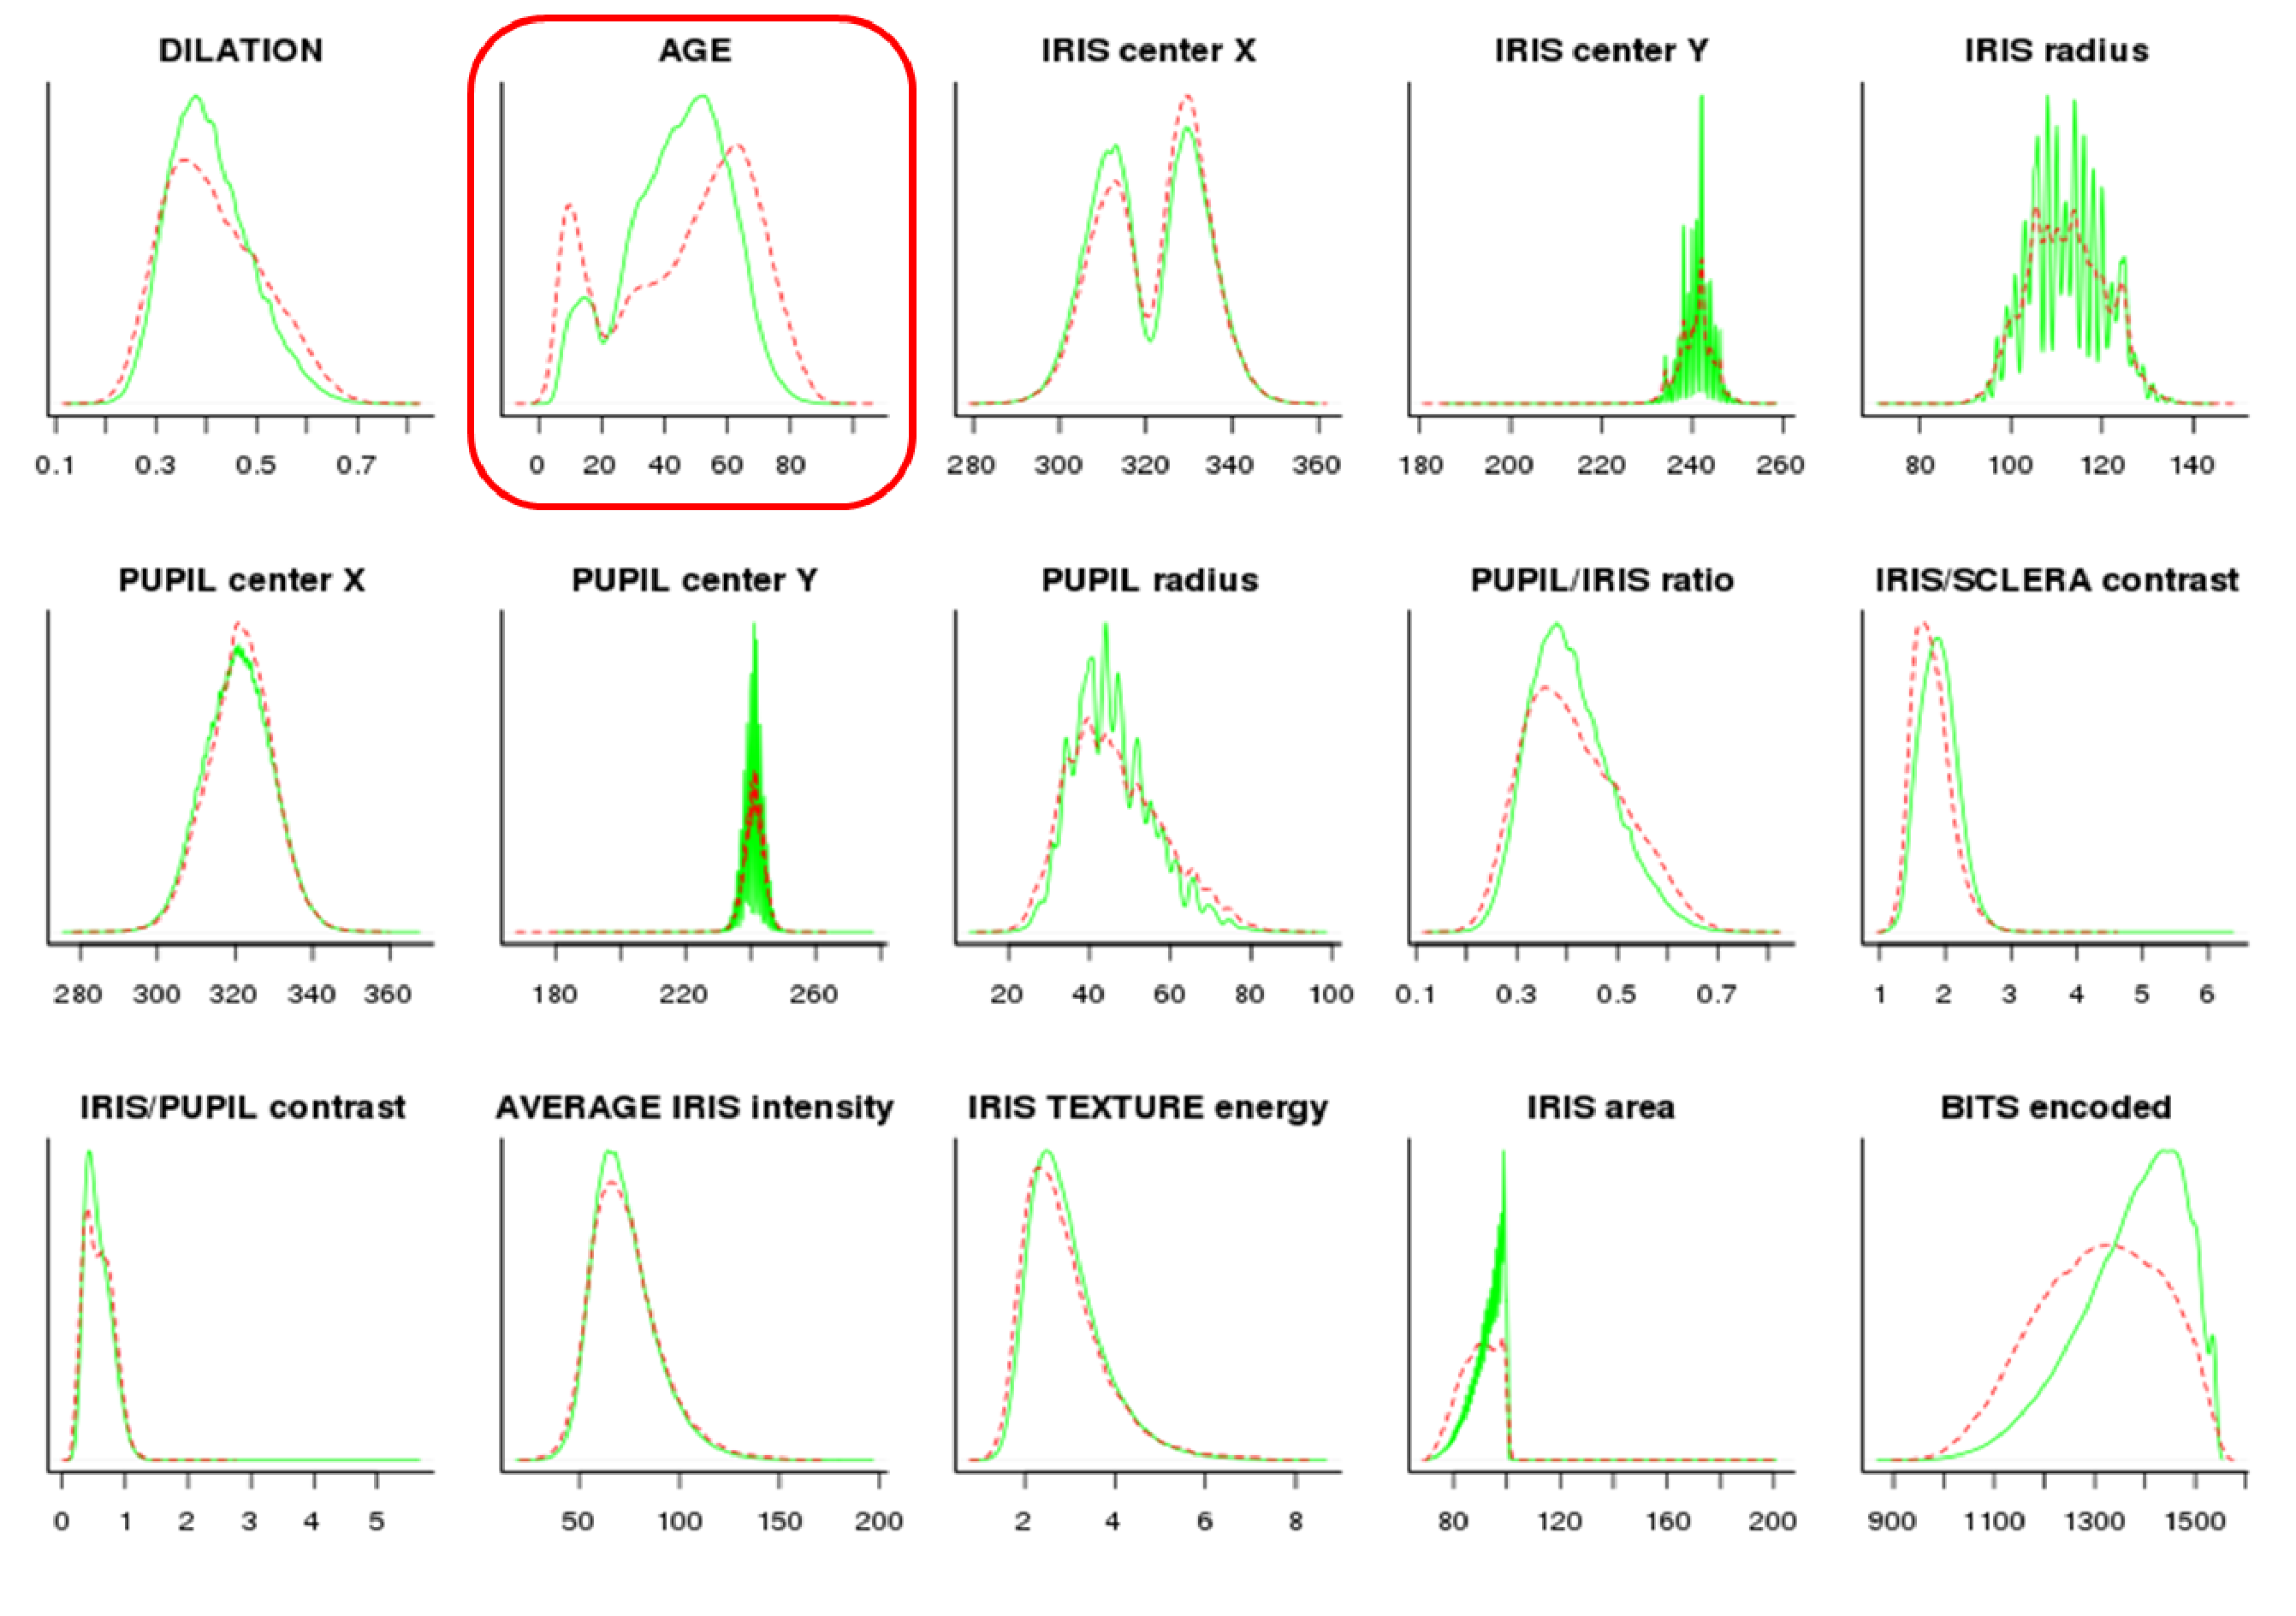
\includegraphics[width=0.52\linewidth]{eps/en-iq-metrics-new.eps} \quad 
%\caption{Relative distribution of Age and Image Quality values  for  ``both eyes'' (green solid line) and ``one eye only'' (red dashed line) enrollments. 
%Observation: Older and younger users are harder to enroll, i.e.,  have more “one eye only” enrollments.
%}
%\label{fDensity_metrics}
%\end{figure}
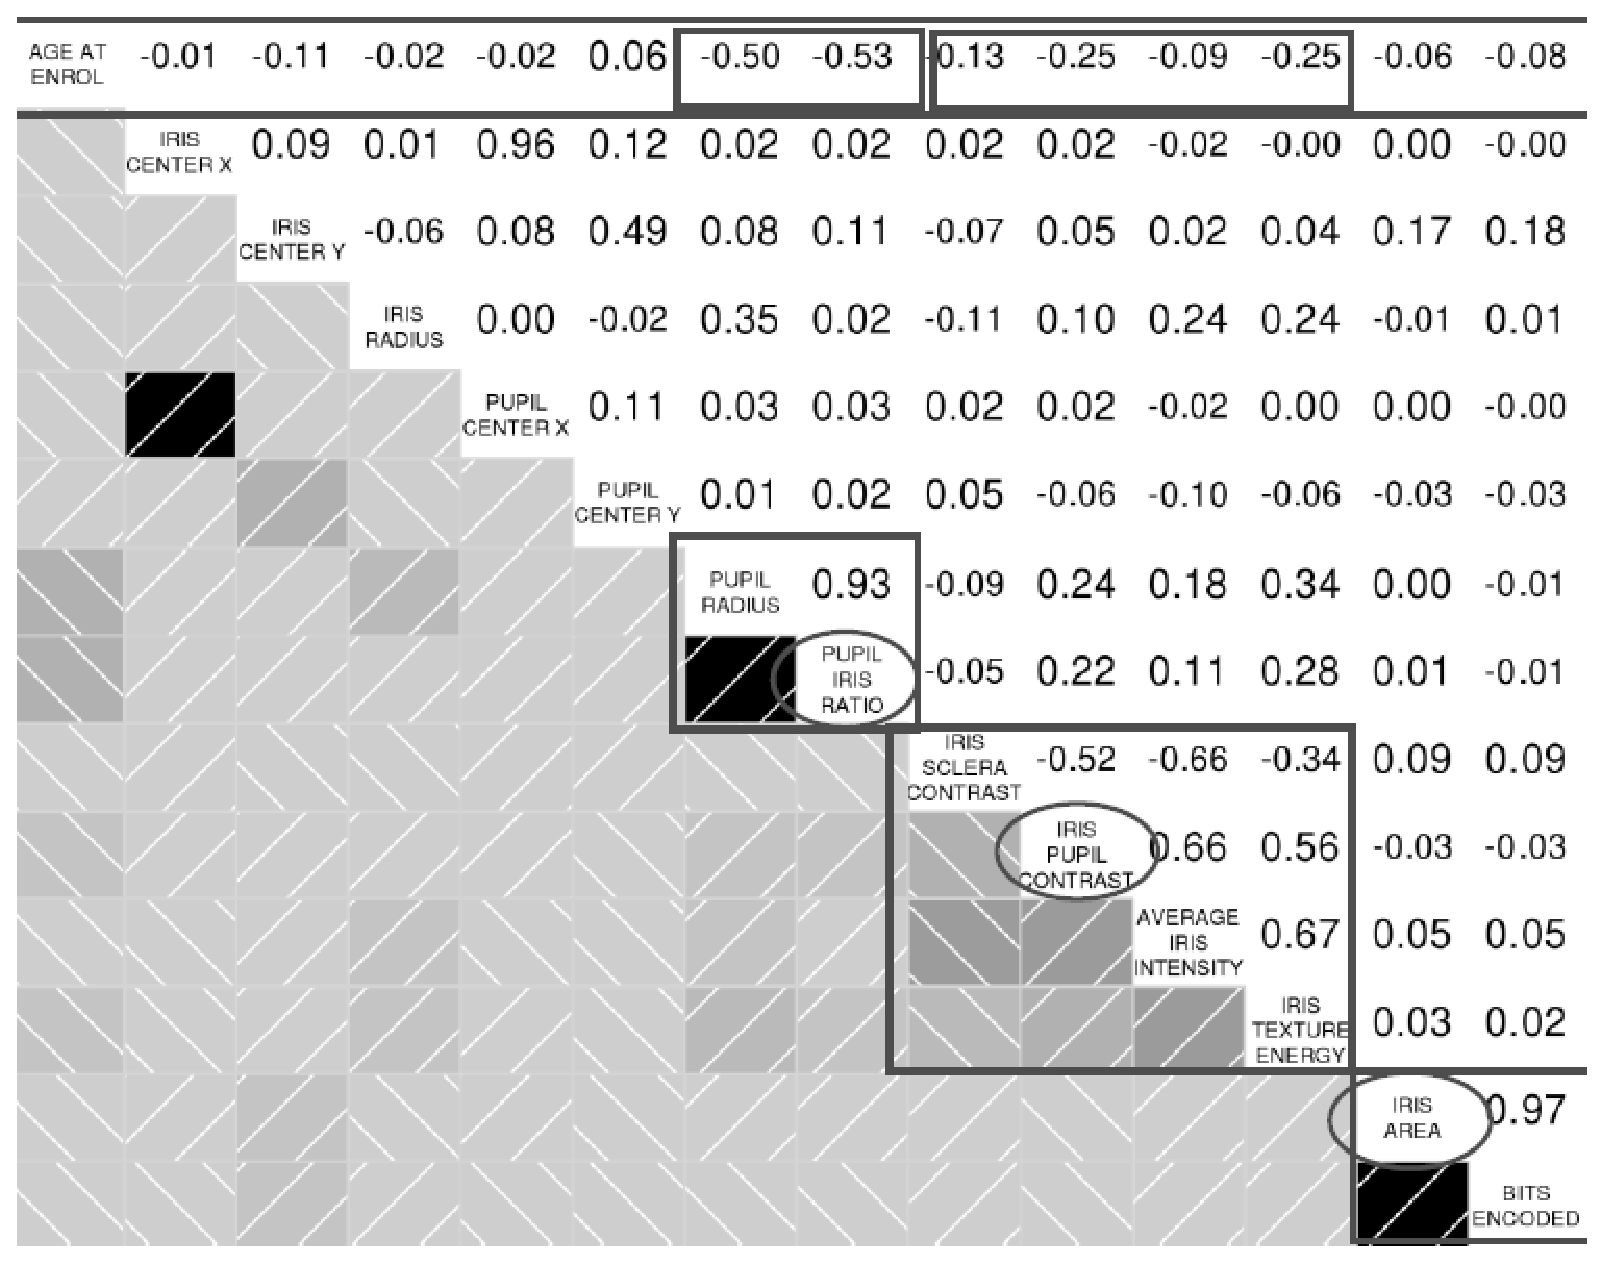
\includegraphics[width=0.45\linewidth]{eps/corr-enIQ.eps} 

%\caption{Correlation of Age and Image Quality metrics at Enrollment.
% (for new “B” cameras). 
%Observation: Three IQ metric groups are distinguished: related to dilation (pupil-iris ratio), eye contrast, and eye openness. Age weakly correlates with Dilation (0.53) and Contrast (0.25).
\caption{Analysis of scores at Enrollment: 
Relative distribution of Age and Image Quality scores  for  ``two-eye'' (solid green) vs. ``one-eye'' (dashed red) enrollments (shown at left);
Correlation of Age and Image Quality scores (shown at right). 
Data from new ``B'' cameras are used. 
}
\label{fCorrelationAgeIQ}
\end{figure*}



\section{Methodology for analyzing the performance of NEXUS kiosks}
\label{s.methodology}


This section presents one of the key results of our study, which shows that the performance of the system varies considerably among the subjects and that subjects who experience problems with the system use it much less than others. 
Based on this finding, methodology for subject-based performance analysis is developed to allow one to investigate the factors affecting the system performance. The taxonomy for categorizing such factors is established.
%and which needs to be taken into account when analyzing the effect of various factors on system performance.

\subsection{Variation of performance among subjects}
%\subsection{Variation of kiosk usage difficulty among subjects}

%\subsection{Key observation} %Performance metrics}

As mentioned in Section~\ref{s.description}, the OPS-XING dataset does not contain the data about travellers who were rejected by the kiosks. 
Therefore, the following two metrics are used to
%estimate the percentage of 
stipulate the number of travellers who have  experienced 
%a higher than normal level of 
difficulty in using the system, 
knowing that some of them used the system only once and some used it more than a hundred times, with 942 passages being the largest number of passages for a subject.


%Criteria
\begin{itemize}
\item       Metric 1:  Traveller's  average number of $Attempts$  is higher than 1.5 (i.e., s/he is over 50\% likely to be rejected by the system from the first attempt).  
%Note that the maximum number of allowed attempts is three.
\item       Metric 2: Traveller's  minimum matching score $HDNORM$ is higher than 0.2.  
%Note that the HD threshold for accepting the person is 0.27.  The transactions that have HD > 0.27 results in rejection, in which case the data is not recorded.
\end{itemize}
%kiosk usage difficulty by travellers.

\cmt{
To conduct the analysis, the following two metrics were computed using data from all travellers, knowing that some of them used the system only once and some used it more than a hundred times, with 942 passages being the largest number of passages for a subject.

\begin{itemize}
\item      Metric 1: The proportion of travellers  who more likely than not are rejected by the system, i.e., for whom the average number of $Attempts$ %$<Attempts>$ 
is higher than 1.5. 
%Note that the maximum number of allowed attempts is three.
\item       Metric 2: The proportion of travellers  who have minimum matching score $HDNORM$ higher than 0.2.  
%Note that the HD threshold for accepting the person is 0.27.  The transactions that have HD > 0.27 results in rejection, in which case the data is not recorded.
\end{itemize}


}

The first metric relates directly to the border wait time, which
is a  performance metric that the agency needs to minimize. 
This metric however may not  always show the actual number of attempts taken by a traveller (e.g., as described in Section~\ref{s.description}, when a traveller 
tries different kiosks or different sessions at the same kiosks, the number of attempts from the last session is recorded only). 
The second metric addresses this issue, as it allows one to estimate the difficulty of using the kiosk  under situations when the number of recorded attempts is the same.  

%Figure \ref{fHDhisto}-b) shows Tukey's five number summary  and  distributions of the $HDNORM$ values  when recognized from the first, second and third  attempt. 

As highlighted in Section \ref{s.HDvsAttm}, the $HDNORM$ metric correlates with the $Attempts$ metric (the more attempts it takes the traveller to be recognized, the worse is the HD value). This allows one to use
$HDNORM$ metric as a proxy performance metric for kiosk performance instead of $Attempts$.
%Therefore, it can be used when analyzing the effect of factors on system performance.

%It is noted that when a traveller is not recognized within three attempts, s/he is given a choice of trying again (i.e., starting a new passage attempt), in which case the system will log his/her interaction with the system as a completely new transaction. That is, a person who is recognized on the fourth attempt is logged as if s/he is recognized on the first  (4 minus 3) attempt. This creates a bias towards a lower number of attempts. However, as seen from the figure, the difference in HD distributions is still very noticeable.


Table \ref{fNumberBAd} shows the  number of travellers who used the system different number of times and the percentage of them who experienced the ``difficulty'' using it, where the difficulty is defined using the two metrics described above.
%  Metric 1 – by a high average number of attempts (<Attempts> > 1.5) and Metric 2 - by a high minimum HD score (HD.min > 0.2). 
%Table 5‑1 provides the actual numbers of the plotted statistics using minimum HD score metric. Additional graphs and tables are provided in Appendix A. 

It is observed that travellers who experience ``difficulty'' in using the system use it much less than those who do not.
Therefore, any performance evaluation results obtained by 
aggregating transaction metrics,
%averaging over all transactions, 
such as those obtained in previous analysis of the OPS-XING dataset \cite{irexVI}-\cite{Bowyer-BTAS2016}, will be highly skewed towards ``better'' performing subjects.
In order to provide an objective picture of the system performance quality, 
\textit{subject-based performance }analysis is required.
%, which is 
%Subject-based performance analysis of a biometric system is 
%based on the metrics that measure  the number of subjects who are falsely matched/non-matched by the system, as opposed to transaction-based analysis, currently established by the ISO and used by industry [18], which is based on measuring the number of  matched/non-matched transactions, is required.

In contrast to the \textit{transaction-based analysis},  established by the ISO and currently used by industry \cite{ISO}, which answers the question: 
\textit{``How many times did the system reject a person?''}, 
%\textit{``How many rejects were produced by the system?''}, 
the \textit{subject-based analysis} answers the question: 
\textit{``How many persons were rejected by the system?'' }
%How many technology quitters does the system generate?}
%The current industry evaluation standard  addresses the first question. 
%For benefits-driven biometrics applications however it is the the second question  that is more important.



\begin{figure*}[!t]

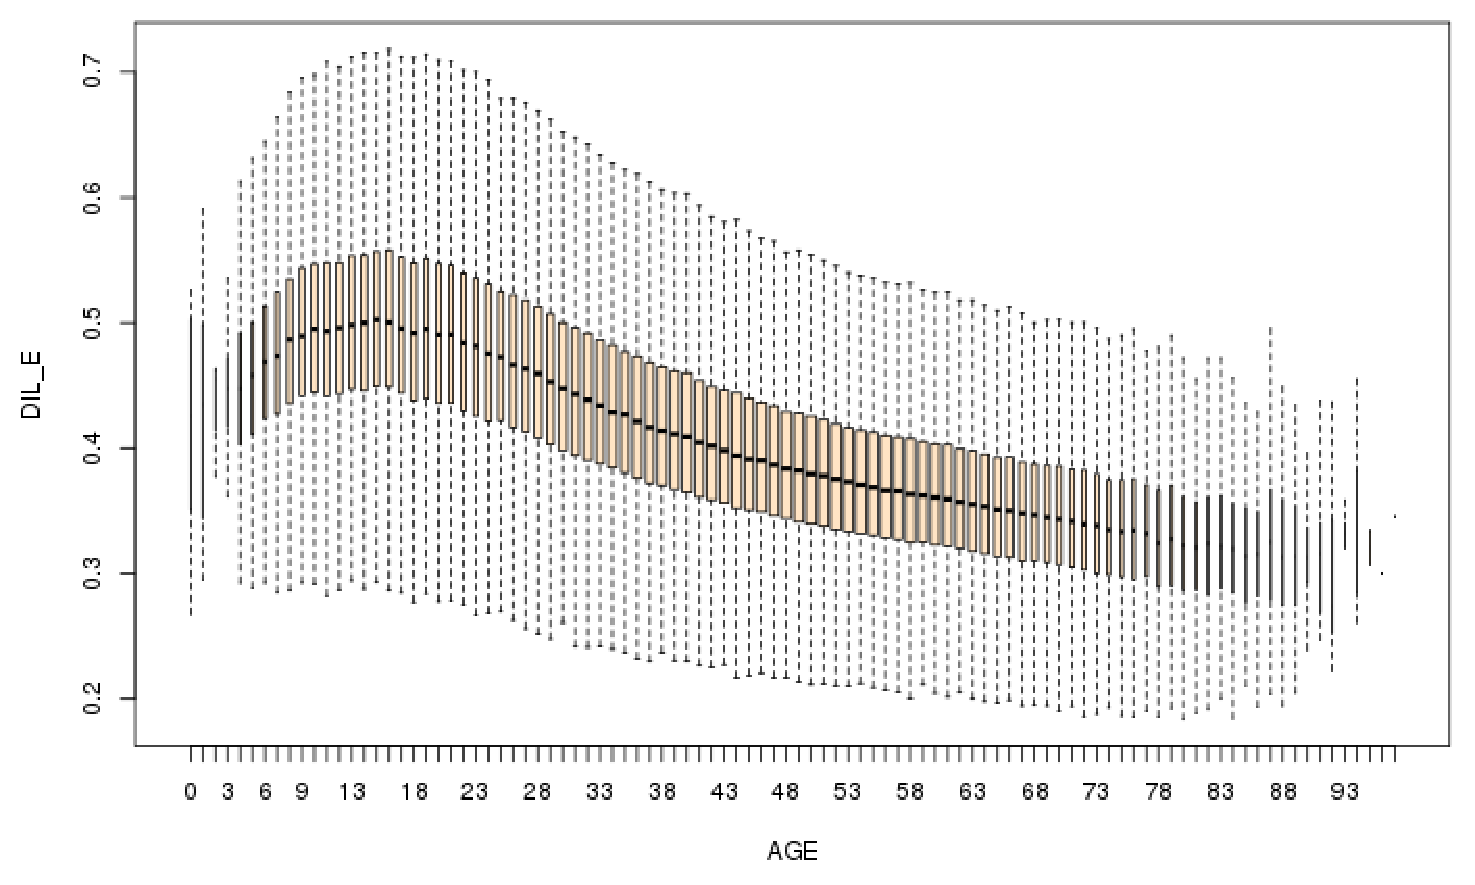
\includegraphics[width=0.5\linewidth,height=1.1in]{eps/21DIL_E=f(AGE)-boxplot(Cam=B).eps}\quad
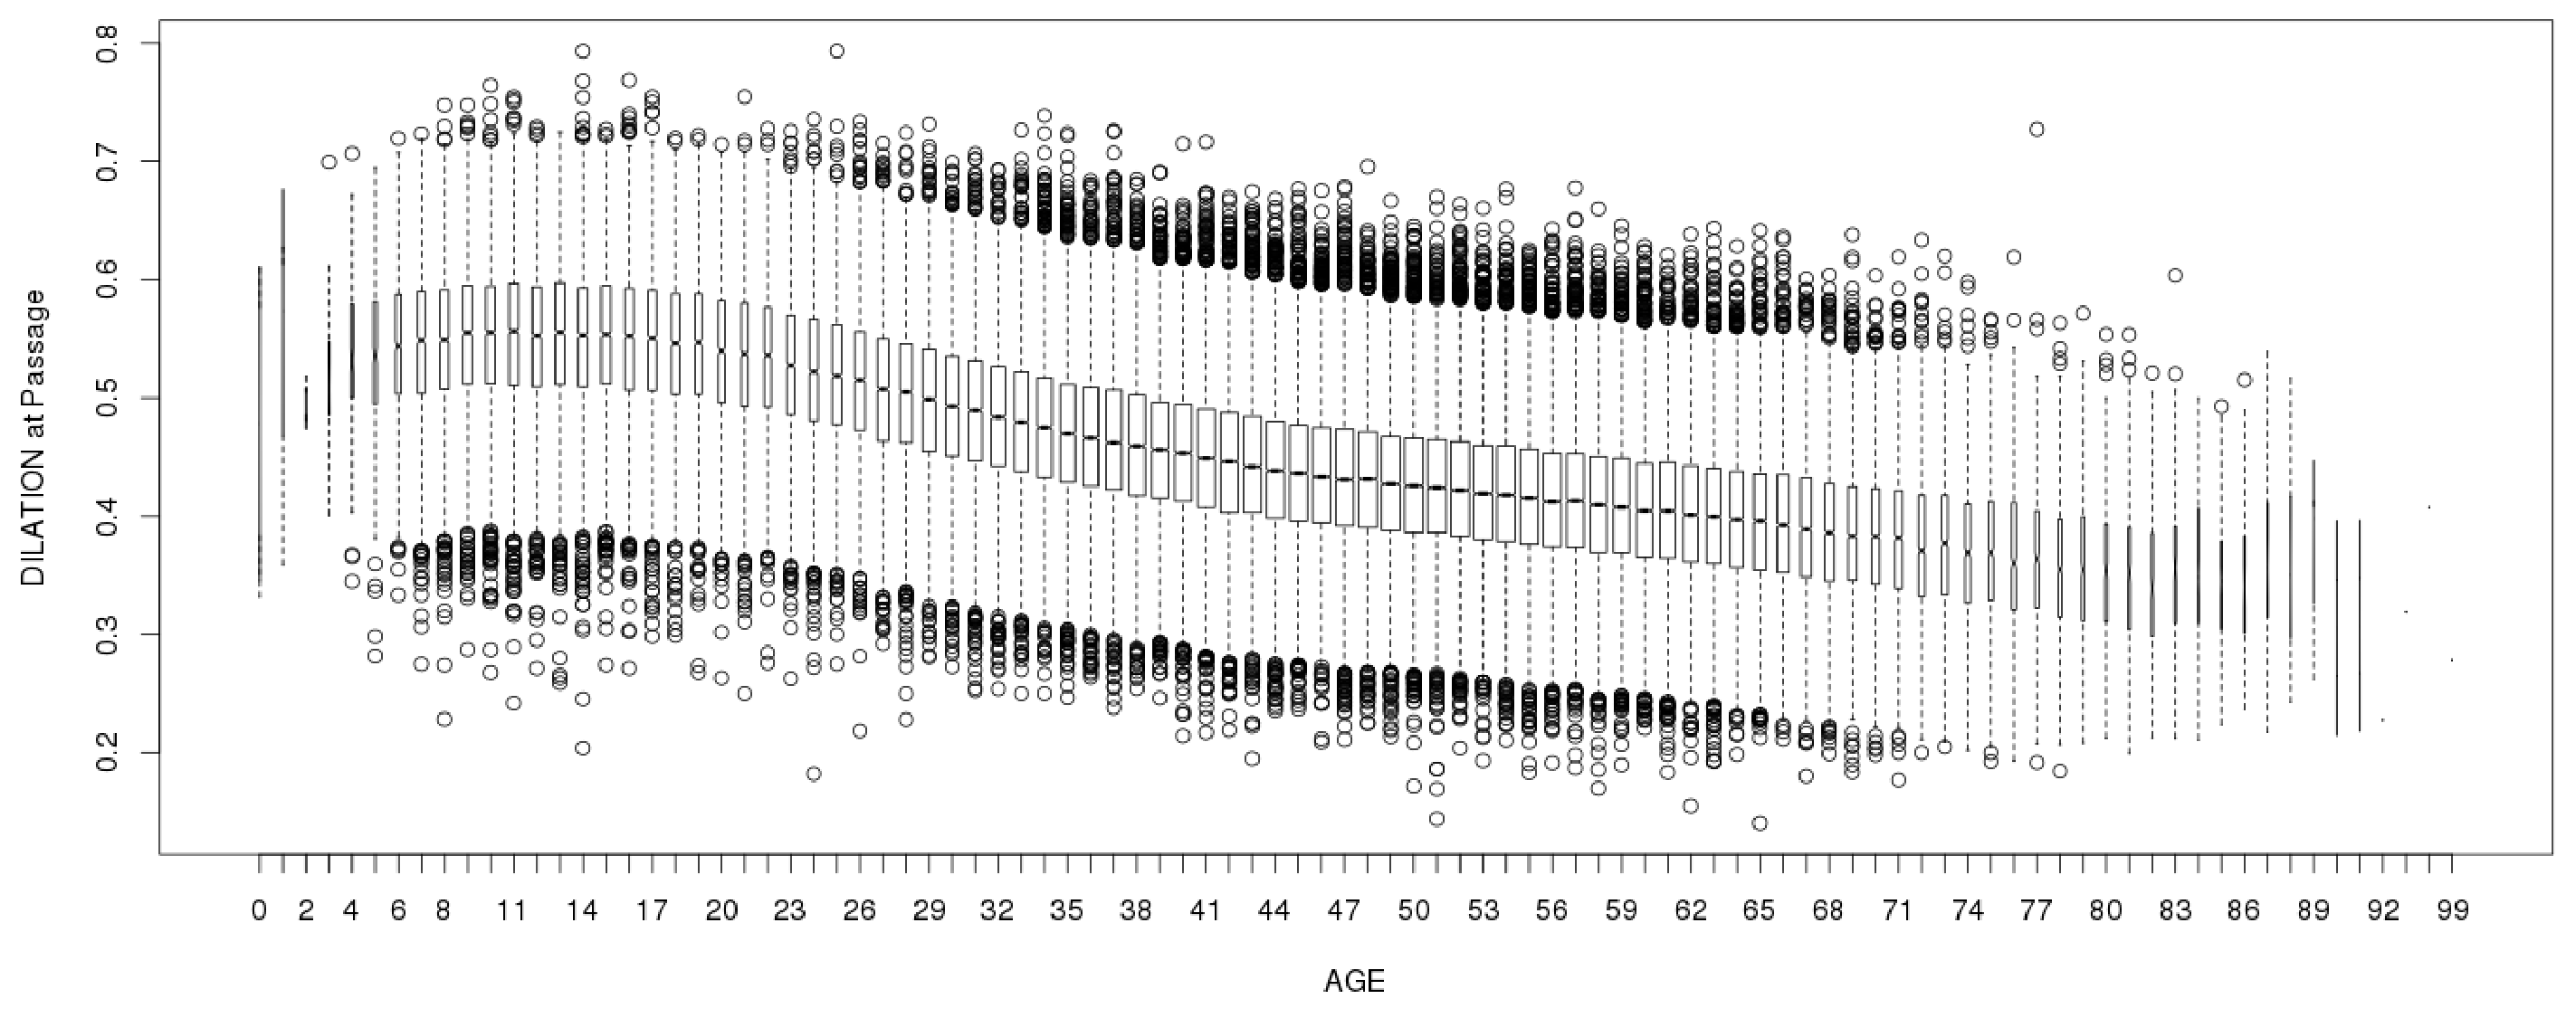
\includegraphics[width=0.5\linewidth,height=1.1in]{eps/DIL-PA.eps} 
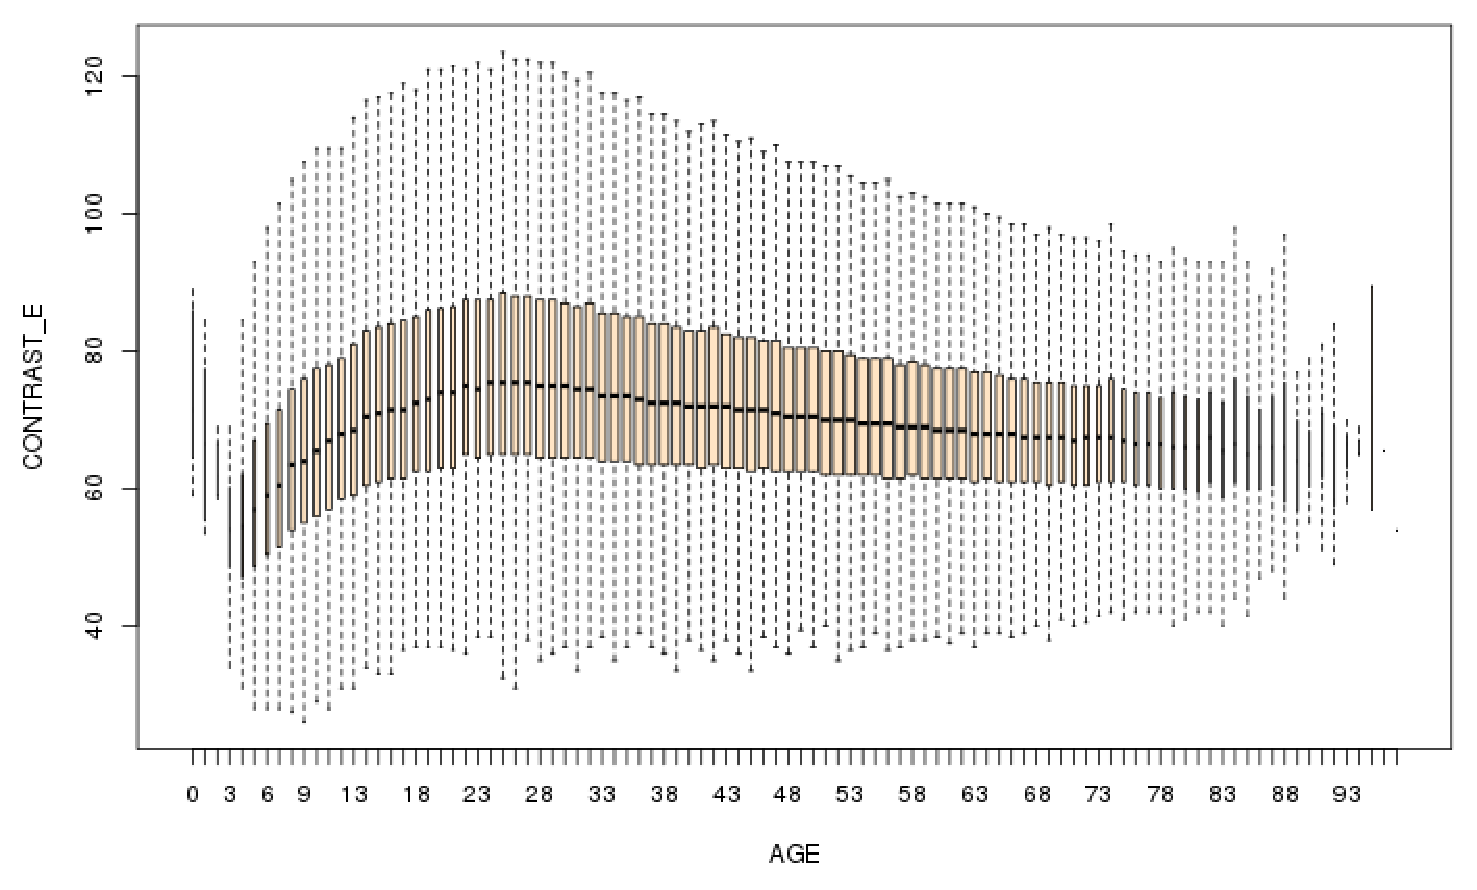
\includegraphics[width=0.5\linewidth,height=1.1in]{eps/21CONTRAST_E=f(AGE)-boxplot(Cam=B).eps}\quad
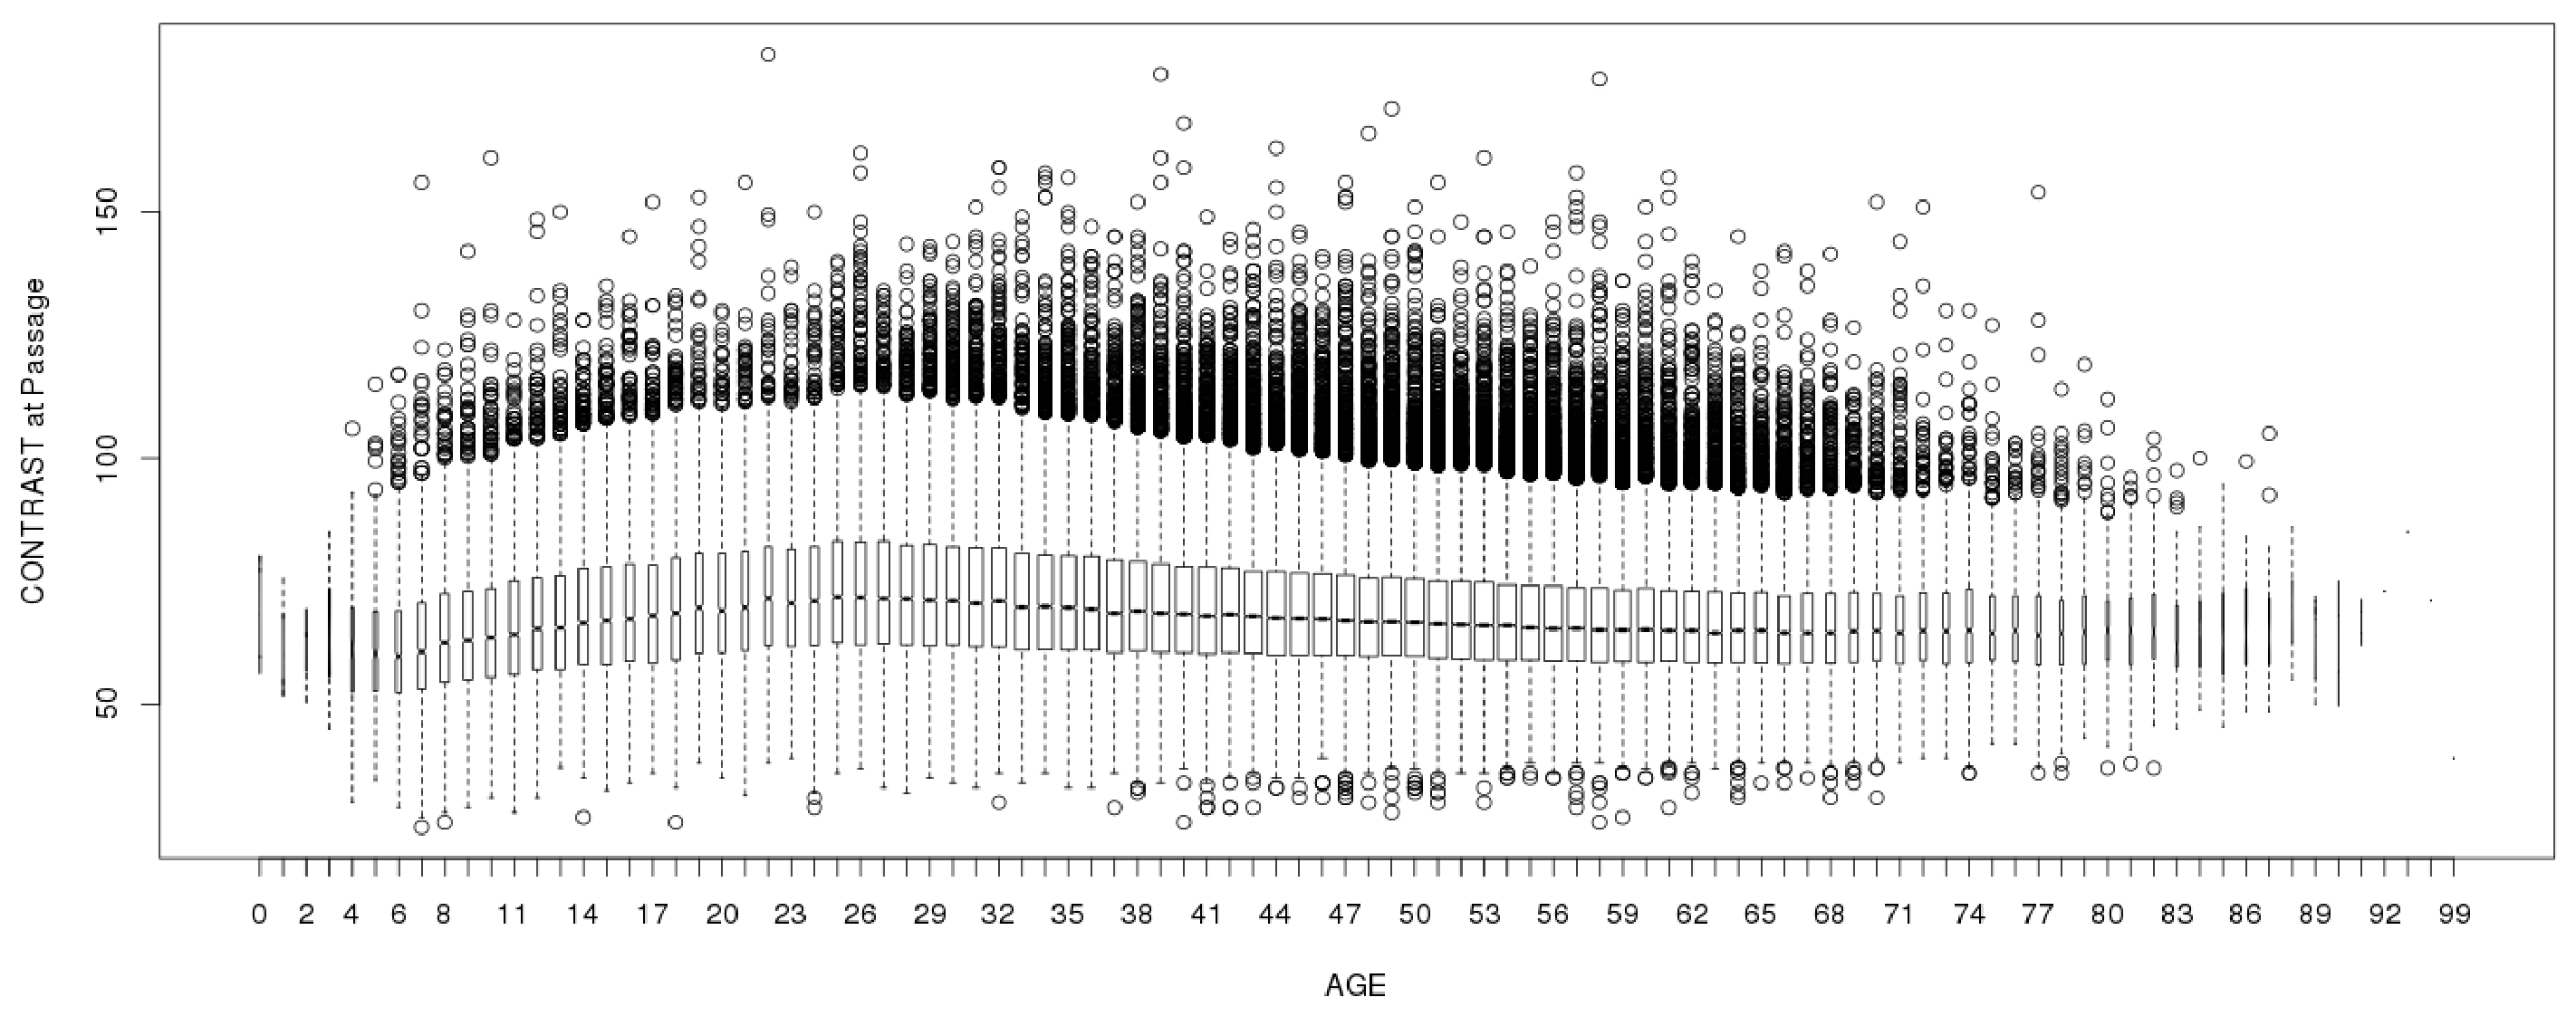
\includegraphics[width=0.5\linewidth,height=1.1in]{eps/CONTRAST-PA.eps}
%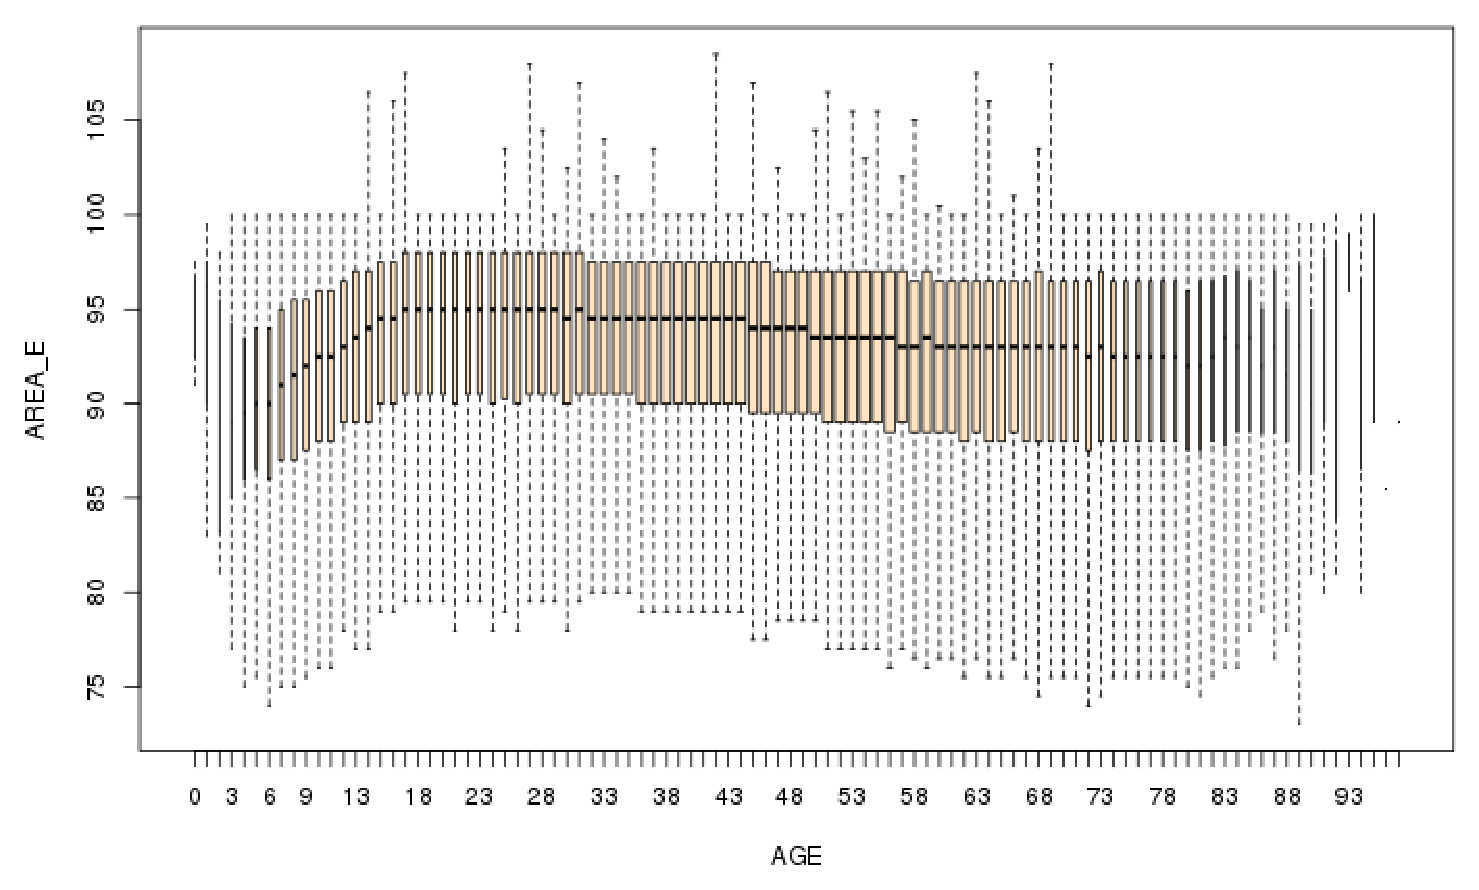
\includegraphics[width=\linewidth,height=1in]{eps/21AREA_E=f(AGE)-boxplot(Cam=B).eps}
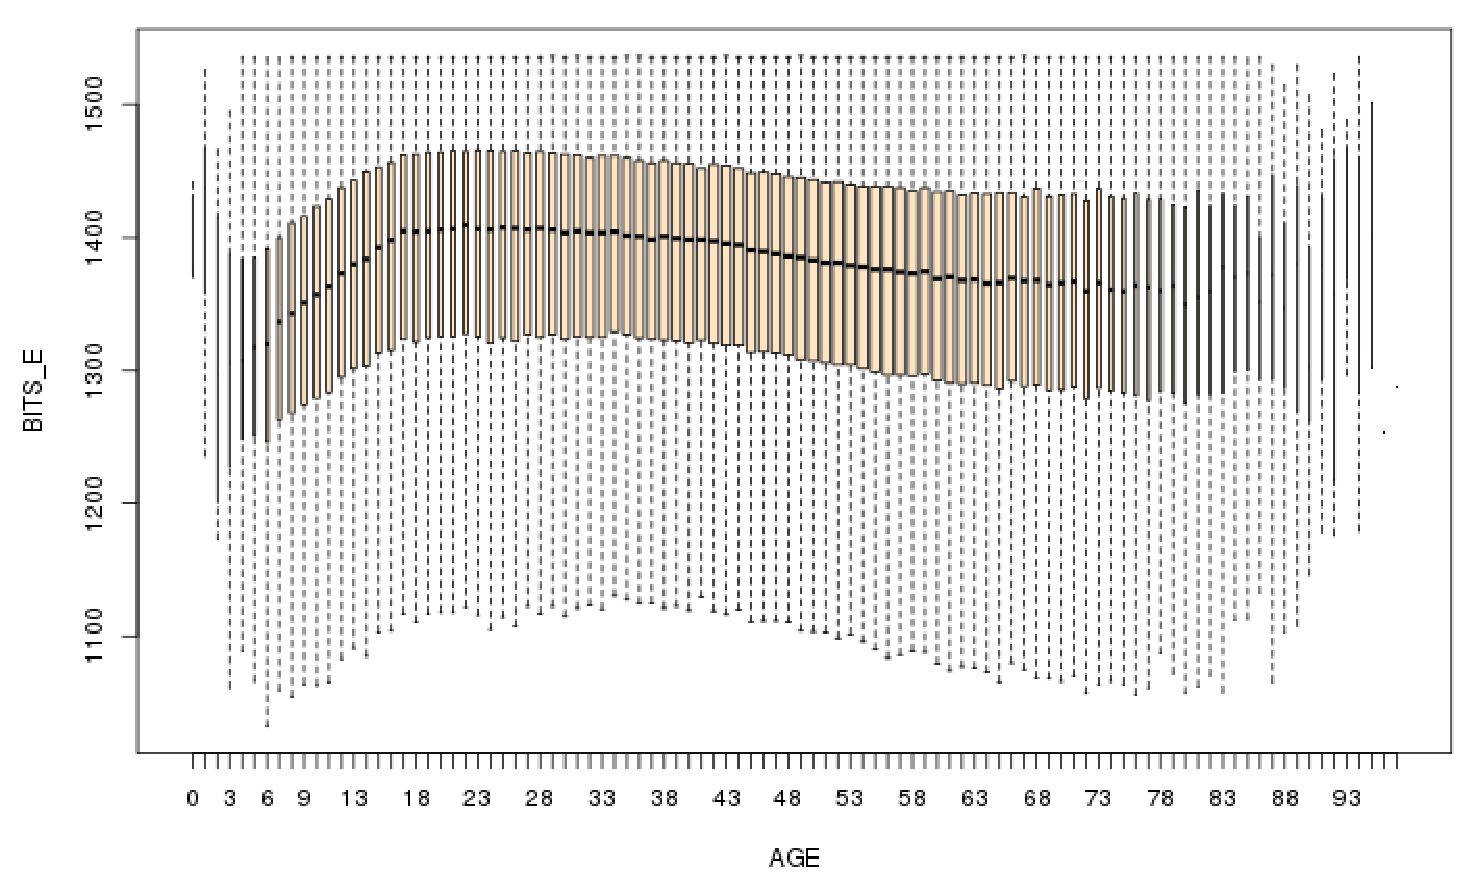
\includegraphics[width=0.5\linewidth,height=1.1in]{eps/21BITS_E=f(AGE)-boxplot(Cam=B).eps}\quad
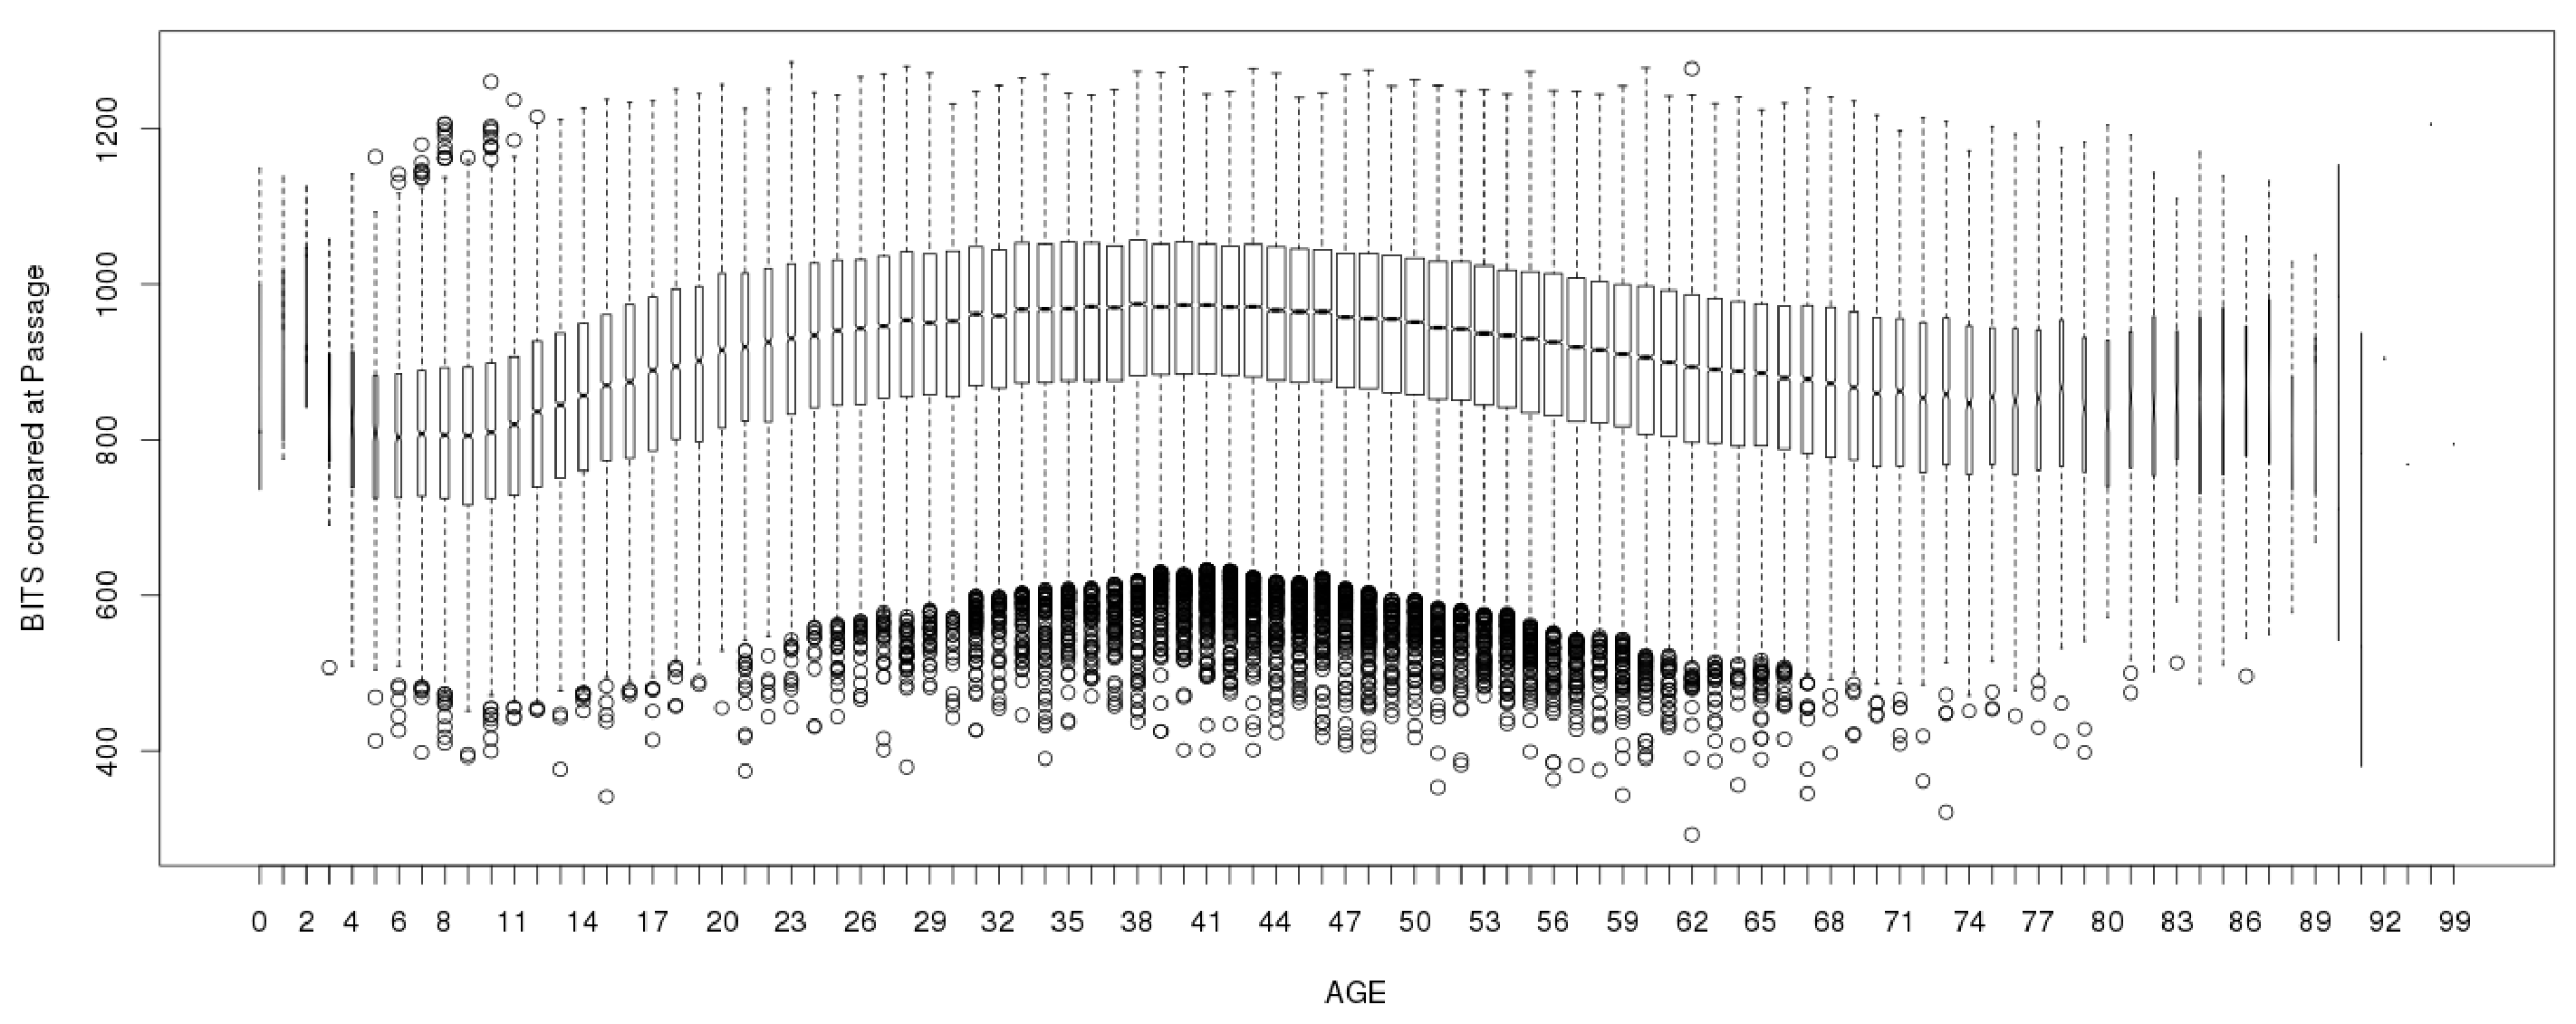
\includegraphics[width=0.5\linewidth,height=1.1in]{eps/BITS-COMPARED.eps}\\ 

%\vspace{1pt}
%\hrule
%\centerline{---}
\vspace{5pt}

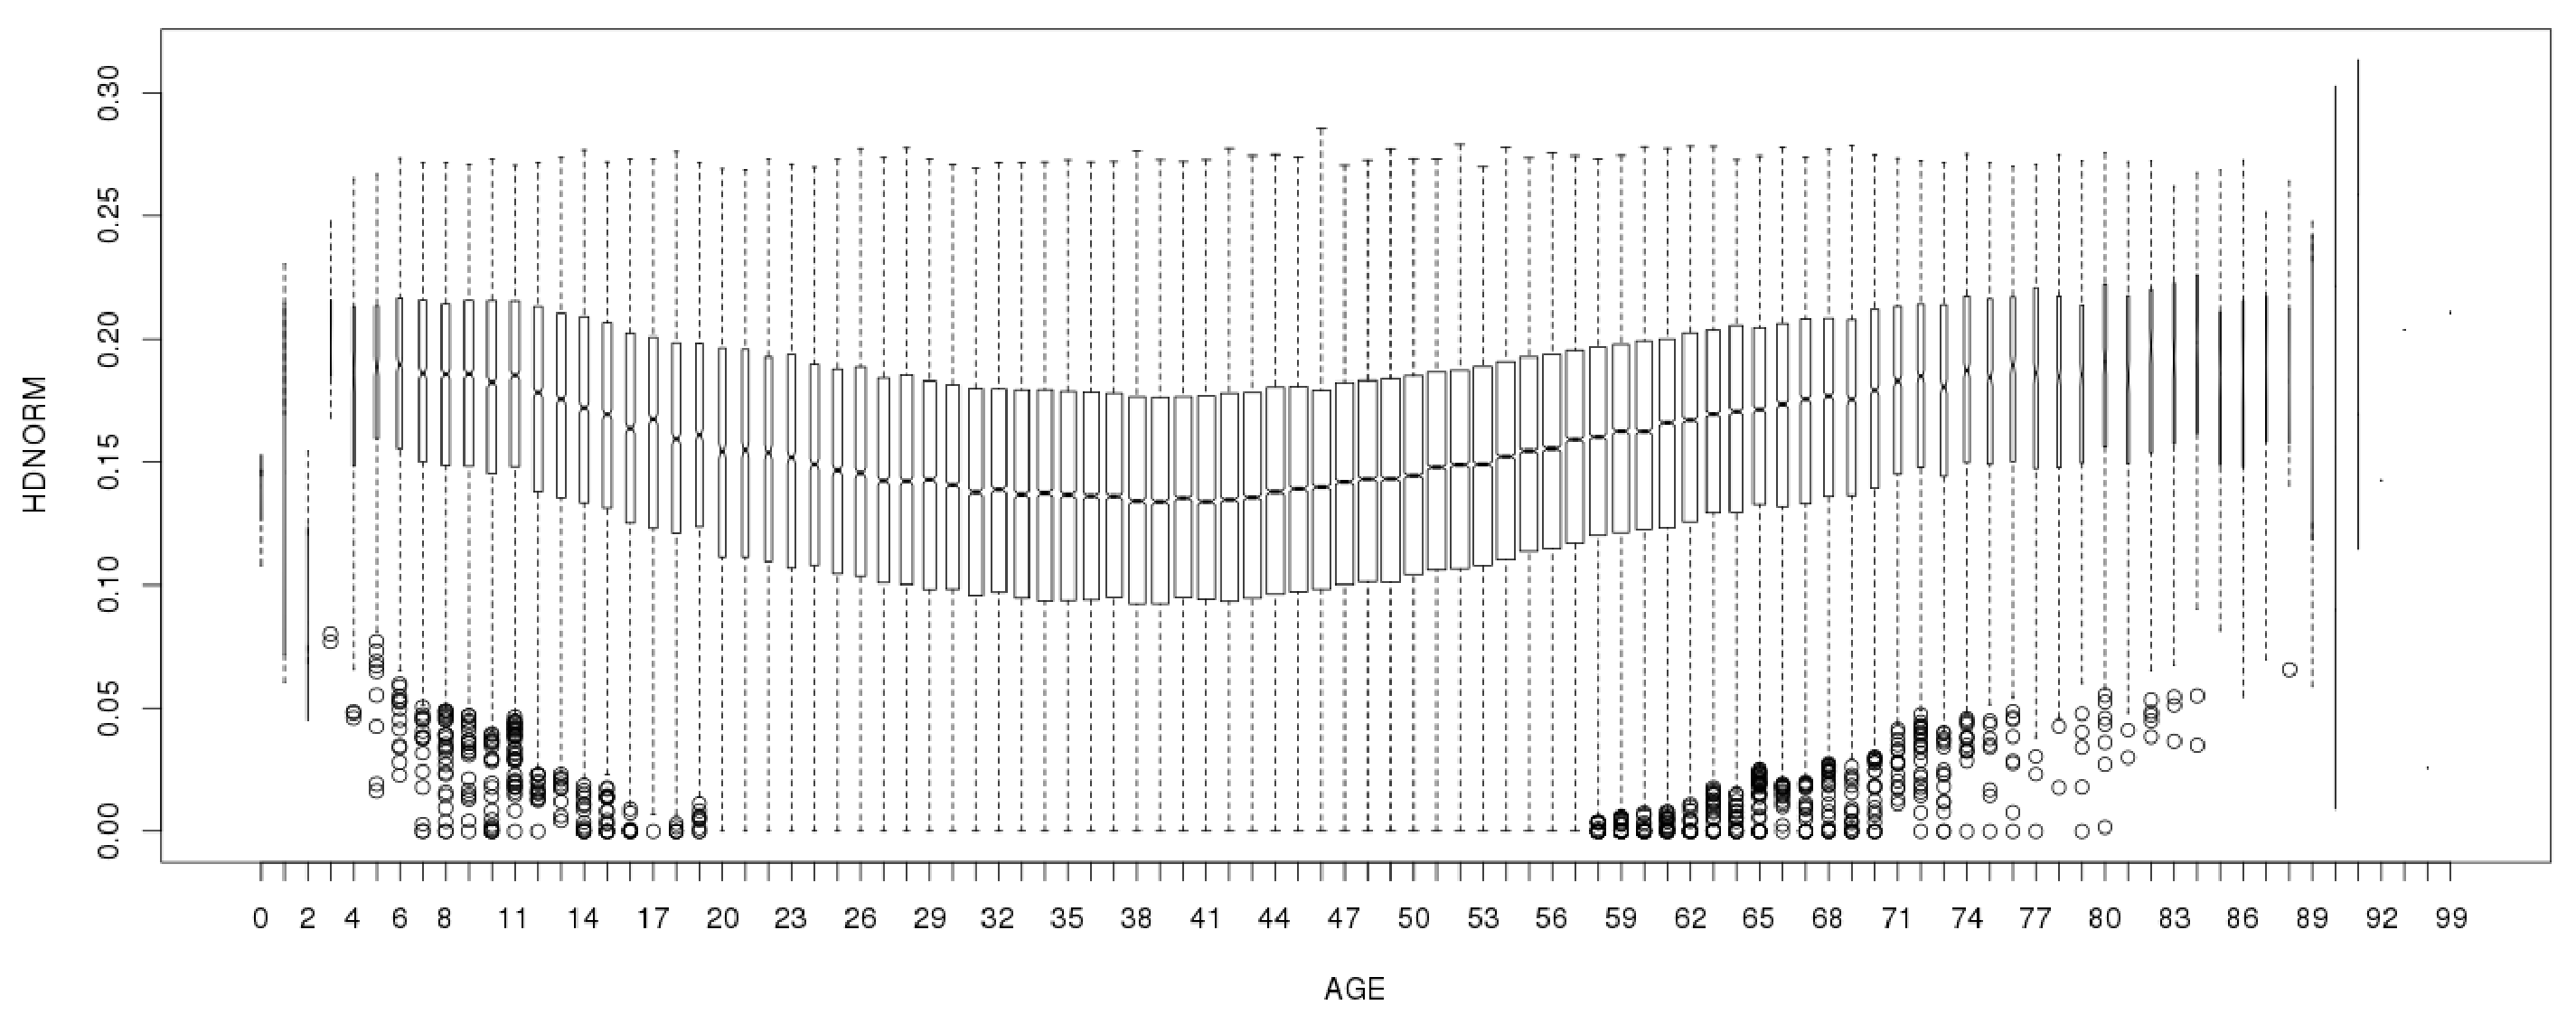
\includegraphics[width=0.5\linewidth,height=1.1in]{eps/HDNORM.eps}\quad
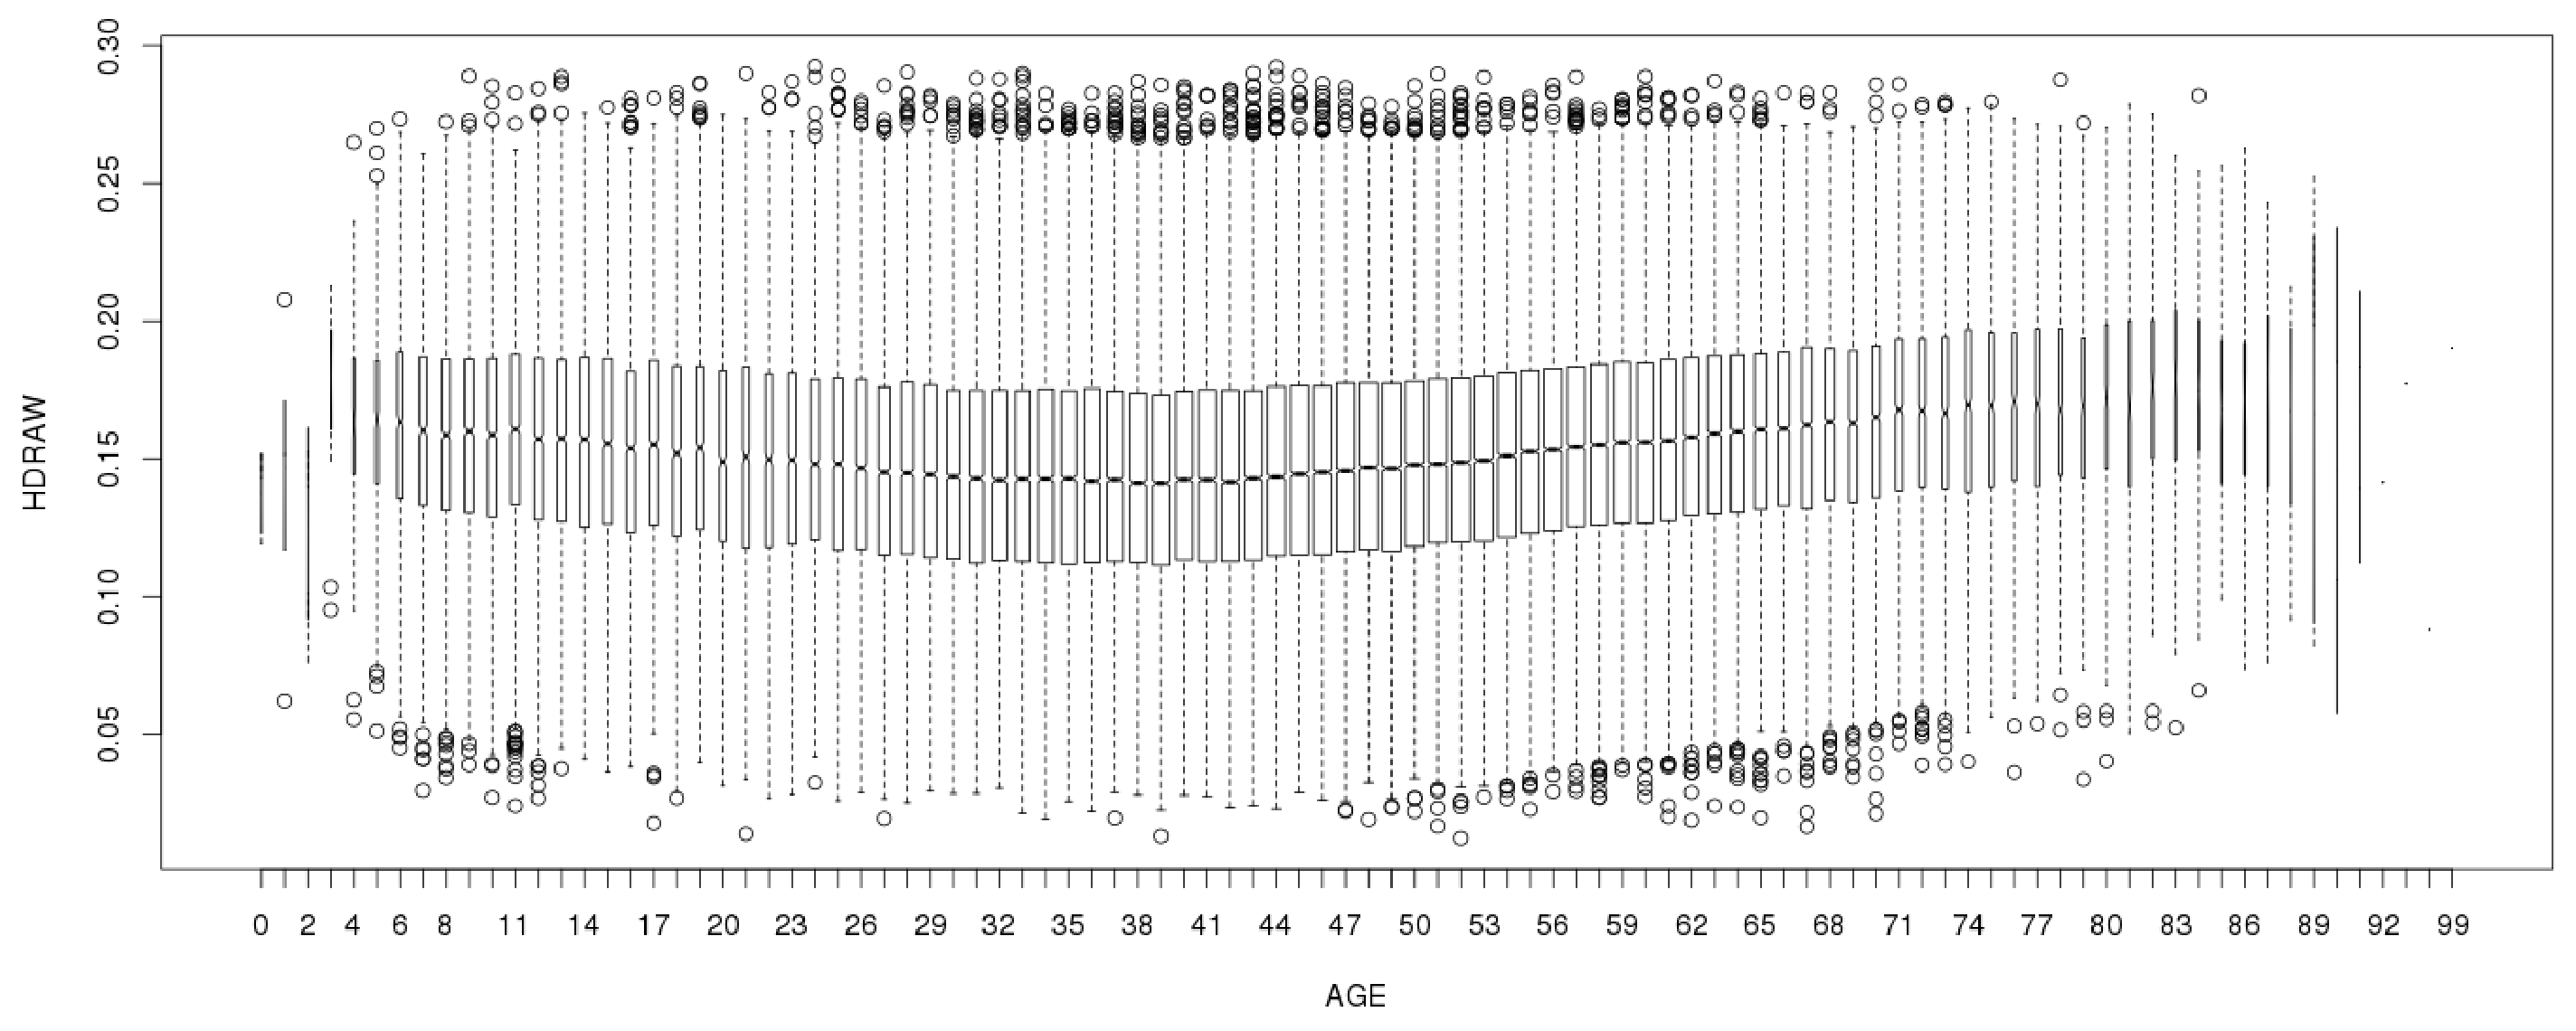
\includegraphics[width=0.5\linewidth,height=1.1in]{eps/HDRAW.eps} 
\caption{Variation of Image Quality and Matching Scores by age.  
Boxplots on the top show  the distribution of Dilation, Contrast, and Number of Bits Encoded / Compared scores for each age --
at Enrollment (left) and  Passage (right). Boxplots at the bottom show  the distribution of HDNORM and  HDRAW scores at Passage.
Box width is proportional to the population size. 
Data from new ``B'' cameras are used. 
%Data from travellers enrolled with new  ``B''  cameras are used.
\label{fHDpassage}}
\end{figure*}




\subsection{Subject-based performance analysis }
\label{s.s-b}

%The fact that some people are intrinsically much harder to recognize than others by a biometric system is well known to biometric system developers. Adversely affecting some groups of biometric system users, this phenomenon is called ``biometric menagerie'' or ``Doddington Zoo'', according to the original work of NIST researchers who discovered and reported it on voice recognition systems \cite{Doddington}. 


Subject-based variation of biometric performance
%, including due to the ``menagerie'' phenomenon, 
is well studied for voice and face modalities \cite{Doddington,Poh}. It has been much less documented and analyzed for the iris modality.  
The major first evidence of subject-based variation of biometric performance in iris systems 
%and the recommendation to improve  the evaluation standards to take it into account
was presented in our earlier work in 2011 \cite{Gorodnichy2011} and has become since then an important guiding principle for us in performing evaluation of biometric systems.


As a general rule for conducting subject-based analysis the following approach is used.  All performance metrics $X$ that are computed for a population
%, such as the average number of Attempts $<ATMPS>$, average Matching Score ($<HD>$) etc, 
are computed using the averages obtained separately for each individual (Eq. \ref{1.2}), as opposed to  
 using averages over all individuals of the entire population (Eq. \ref{1.3}), done in the transaction-based analysis.

%The application of this approach is shown in next section.

\begin{eqnarray}
<X>_{subject-based} = { \sum_{s\in \ subjects} ( <X_s> ) \over {\rm \#\ subjects} }  \label{1.2} \\
<X>_{transaction-based} = { \sum_{s\in \ transaction}  X_t   \over {\rm \# transactions} } \label{1.3} 
\end{eqnarray}

In general, one should expect transaction-based metrics to be different from subject-based one, skewed towards  the average metrics of the most frequently observed subjects.
%What makes some subjects more susceptible to system failures than others is an important question and it is analyzed next.
%There are many factors that can lead to varying performance among subjects. 
By conducting subject-based analysis, one  is able to better decipher the factors that negatively affect the system performance.
%, thereby making it possible to improve it.
These factors are categorized and analyzed next.
%The key performance metrics $X$ that can be analyzed for the OPS-XING dataset are the ... These are analyzed below.

%\subsection{Analysis of factors}


\subsection{Factor categorization}
\label{s.Factors}

From an operational perspective, it is important to distinguish factors by their prime cause.
Using the approach that we first developed for video surveillance applications 
\cite{GorodnichyVA}, 
the factors that effect biometric systems performance are classified into one of three types according the ``technology-process-subject'' factor triangle: 

\begin{itemize}
	
		\item \textit{Technology-related factors.} This group of factors relate to the general limitations of the technology. They affect all users regardless of the process and user-specific characteristics. Any improvement of the system performance due to these factors requires contacting a vendor and potentially replacing the technology. Aging 
	%	(i.e., change of appearance due to human aging  process) 
		(i.e., deterioration of the technology performance with time) 
		is an example of technology-related factor. 
%		which characteristics. They can be caused by sub-optimal matching formula or other technical difficulties such as mentioned in Chapter 3.  If such factors can be detected, recommendations can be made to technology developers in order to improve the technology.
%Examples:  Aging, dark iris, non-circular pupils. 

			\item \textit{Process-related factors.}  The second group of factors relate to the conditions in which the technology is used. It is normally the responsibility of the organization deploying the technology to make sure that the technology is used under the conditions where it works the best. Kiosk location is a prime source of process-related factors, potentially leading to worse image quality and performance for all users. %, as for example in the presence of direct sun light is critical
			
%			depend on both technology and the user, and normally can be corrected once detected, with or without the engagement of the user.
%Examples: Location of the kiosk, the design of the kiosk, iris capture procedure (camera focus, number of image captures).


	\item \textit{Subject-related factors.} The last group of factors relate to particular characteristics of a person or group of people that make some travellers more vulnerable in operating biometrics systems 
	than others. 
	This includes person's gender, age and  other subject-specific physiological and behavioural 	peculiarities such eye colour, size or shape of  pupil, medical conditions, including wearing contact lenses.
	If such factors are detected, they can be used to improve the performance of the system by either alerting a user (e.g.,  by automatically detecting contact lenses and asking a user to remove them), or by allowing different thresholds for users of different groups (e.g., for the elderly). 
	%age group or gender, or by inviting a user to re-enroll his/her iris.
%Examples: person wearing contact lenses or eye-glasses, age, gender, race.

\end{itemize}

 In the following the effect of these three groups of factors is examined, using the enrollment data and then using the passage data.


\begin{figure*}[!b]
\centering
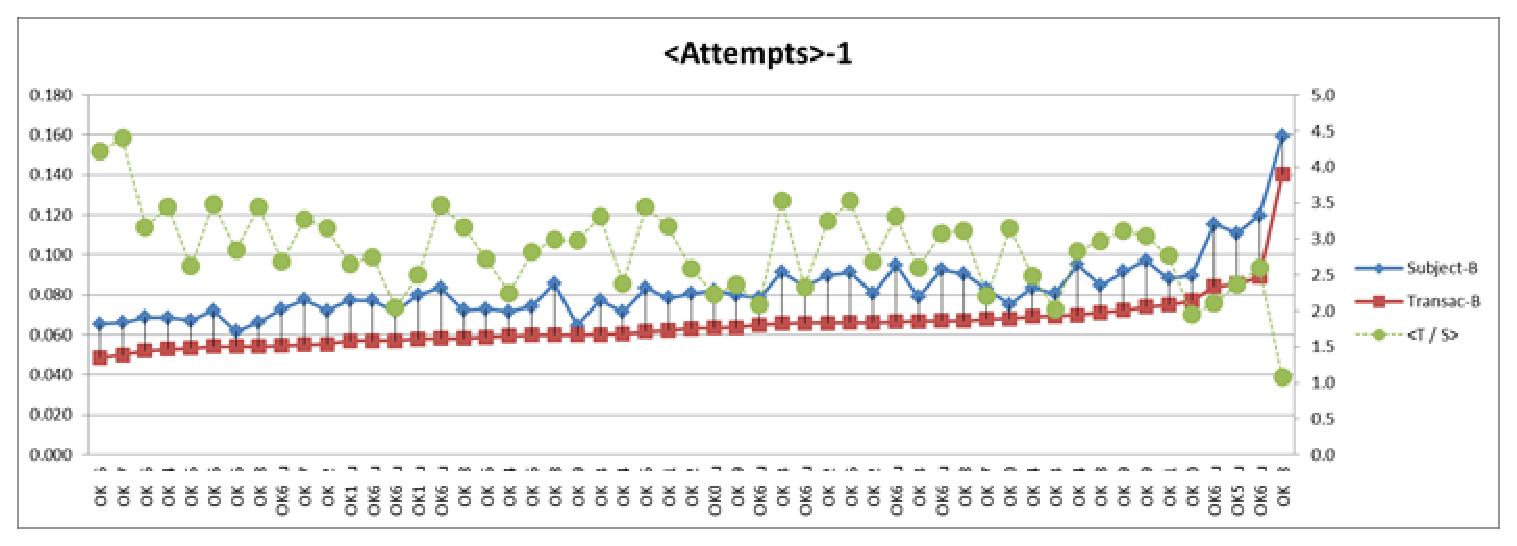
\includegraphics[width=0.50\linewidth,height=1.2in]{eps/image060-hidden.eps}~
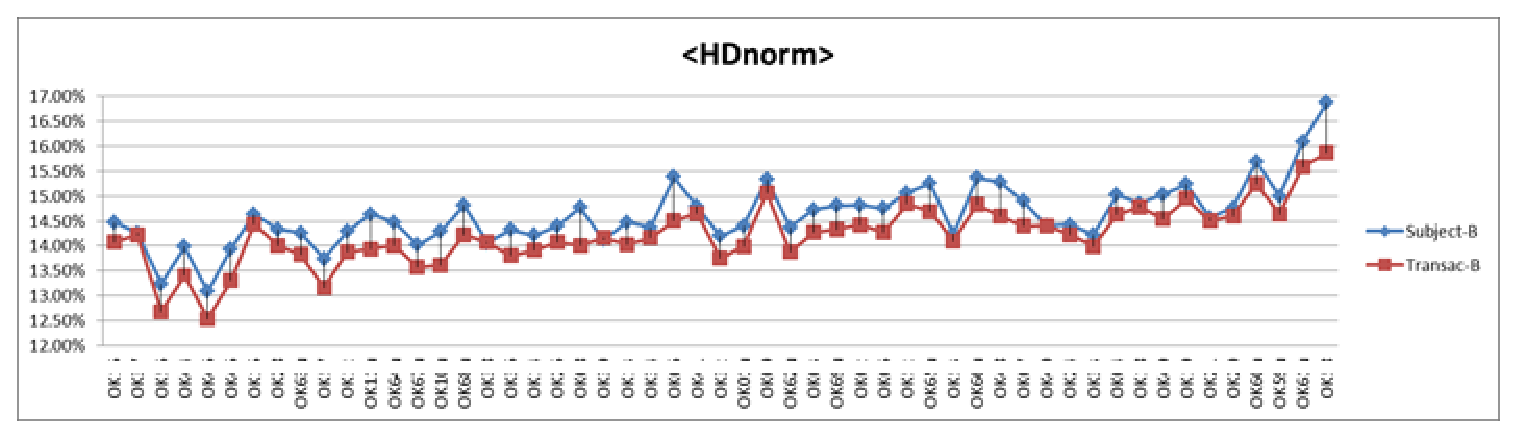
\includegraphics[width=0.49\linewidth,height=1.2in]{eps/image061-hidden.eps} 

\caption{Effect of kiosk location: Performance of NEXUS kiosks measured by the average number of attempts (left) and the average matching score (right), using transaction-based (in red) and subject-based (in blue) metrics, sorted from best performing to worst performing. 
The average number of transactions per subject ($T/S$) is shown (in green).
Kiosks numbers are obscured  to protect airport identities.
}
\label{fKIOSKS}
\end{figure*}




\section{Analysis of Enrollment data}
\label{s.resultsEN}

Enrollment data allows one to examine subject-related factors, specifically the affect of age on image quality.
It does not require subject-based metrics, because all enrolled travellers have exactly one enrollment transaction.




\subsection{Young and elderly have worse image quality and are harder to enroll}
\label{s.IQ-EN-age}

Figure \ref{fBoxplot-IQen} %Figure \ref{fDistributionAge} 
shows the number of NEXUS members who enrolled iris and the percentage among them who could enroll one iris only for each age:
from newborn to 100-year old people.
A dip at  19-20 years of age is explained by the NEXUS program rules where children 18 and under are free to enroll at no charge with parents. 

%Note that 
%As a point of interest,  it is noted that that among NEXUS members  using iris biometrics  there are people of all ages, including newborns and 100-year old people. 


Two important observations are made. 
First, it is seen that the majority of enrolled travellers are between 30 and 60 years old, 
%middle-age people 
and almost all of them ($>98\%$) were able to enroll both irises.

Second, it is seen that 
%In contrast, 
the ability to enroll both eyes is much worse for young travellers and  and diminishes steadily with age for older travellers. 
%This is the indication that image quality monotonically decreases with age starting
This is an indication that image quality of these age groups  is worse than that for middle-age group.
This conjecture is  validated next. 

In order to remove the factors due to camera quality, the data from travellers enrolled with new  (``B'') cameras are used only.
These data counts for over 95\% of the dataset.
The boxplots for Dilation, Contrast, and Number of Bits Encoded values at Enrollment in these data, for each age, 
are shown in Figure \ref{fHDpassage}.

It is observed that dilation monotonically decreases with age for adults, 
which supports the conclusions from \cite{irexVI}.
However, it is also observed that other IQ metrics also slightly decrease with age for adults.
%further supporting the discovered by NIST scientistsThis supports the findingsprevious
%The decrease of Dilation with age is  visible supporting 
The decrease of all IQ metrics for young people is also observed. 
This explains lower number of iris enrollments for older and young users.

In order to further examine the relationship between traveller's Age and IQ metrics at Enrollment, we plot in Figure \ref{fCorrelationAgeIQ} 
the correlation of Age and IQ metrics, and  the distribution of  Age and IQ metric scores at Enrollment - for cases where both irises were captured vs. those cases where  where only one iris was captured.  

The observation is that  older (over 60 years) and younger (under 15 years) users are harder to enroll, i.e.,  have more ``one eye only'' enrollments.
Three distinct IQ metric groups  are also observed --  related to Dilation (pupil-iris ratio), Contrast, and Openness, 
%of which two are found to correlate with Age: Dilation (at 0.53) and Contrast  (at 0.25).
of which the Dilation group correlates with Age the most (at 0.53).

%It is seen that many more middle age travellers are enrolled than young or old travellers, and that younger and older travellers are generally harder to enroll, i.e.  have more “one eye only” enrollments.
%The same figure also shows 
%and the correlation of age and IQ metrics.%

\cmt{
Figure \ref{fCorrelationAgeIQ} 
%\ref{fDensity_metrics} 
shows the distribution for traveller's Age and IQ metrics at Enrollment for cases where both irises were captured vs. those cases where  where only one iris was captured. 
%It is seen that many more middle age travellers are enrolled than young or old travellers, and that younger and older travellers are generally harder to enroll, i.e.  have more “one eye only” enrollments.
%The same figure also shows 
and the correlation of age and IQ metrics.%, measured on new ``B''cameras.
%Figure \ref{fHDpassage} shows boxplots for Dilation, Contrast, and Number of Bits Encoded for each age at Enrollment. 
%The width of the boxes is proportional to the size of the group population.

The following observations are made. 
First, it is observed that older (over 60 years) and younger (under 15 years) users are harder to enroll, i.e.,  have more ``one eye only'' enrollments.
Second, among three distinct IQ metric groups  (related to Dilation (pupil-iris ratio), Contrast,  Openness), Age is found to weakly correlate with Dilation  (0.53) and Contrast  (0.25).
Finally, it is observed that
Dilation monotonically decreases with age for adults,  and  that all  IQ metrics also vary with age for young users. 
This explains lower number of iris enrollments for older and young users. This is also why one may expect worse performance for these groups of people at the Passage stage.
}





%13\% (0.0190/0.15844)
%Two better performing () and two worse performing () airports, with different traffic densities (one has much higher traffic than the other), are chosen and compared to each other, 


%13\% (0.0190/0.15844)
%Two better performing () and two worse performing () airports, with different traffic densities (one has much higher traffic than the other), are chosen and compared to each other, 





\begin{table}[!b] 
\caption{The difference in the average of the HDRAW score. 
\label{t.kiosks-t-test}}
\scriptsize {
%\caption{The 95\% confidence intervals for the difference  in kiosk average score HDRAW computed using subject-based (s-b) and transaction-based (t-b) metrics.}
%\caption{Results of the T-test for pair-wise comparison of kiosks performance. } 
%\small{The table shows 95\% confidence intervals for the difference  in kiosk average score HDRAW, computed using subject-based (s-b) and transaction-based (t-b) metrics.}
%\label{t.kiosks-t-test}
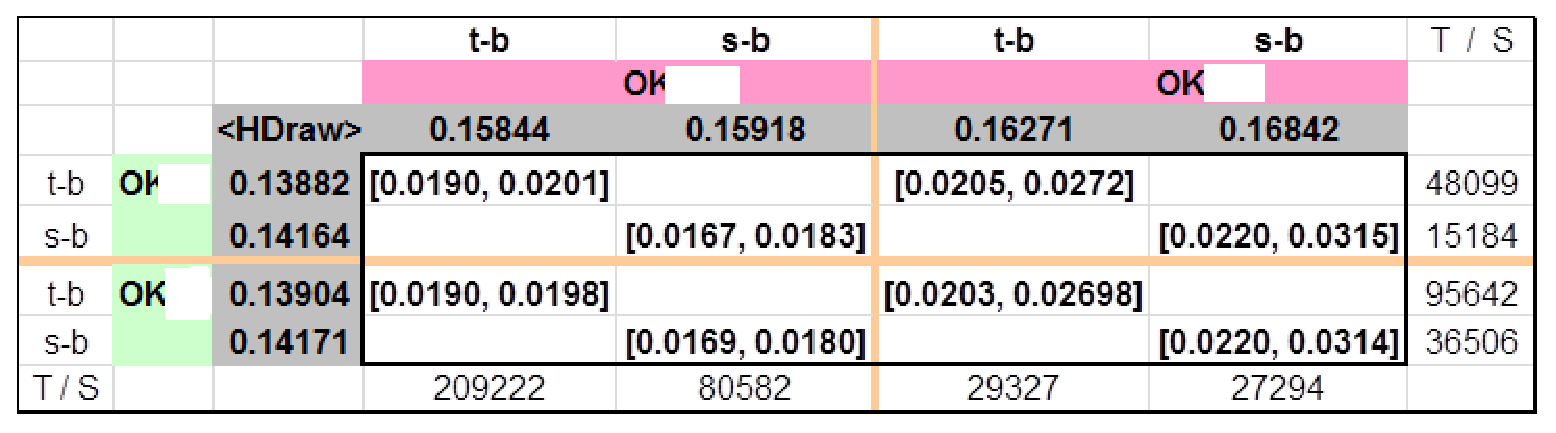
\includegraphics[width=\linewidth]{eps/T-test-kiosks-hidden.eps} 
Note: HDRAW score is computed for two better performing and two worse performing kiosks using  subject-based (s-b) and transaction-based (t-b) metrics. 
%The  95\% confidence intervals for the score difference are shown in the center part of  the table. 
%The number of transactions and subjects (T / S) at each airport are shown on the margin. 
%Actual kiosks numbers are removed from the table to protect airport identities.
}{}
\end{table}






\section{Analysis of Passage data}
\label{s.resultsPA}

\subsection{Variation of performance by kiosk location}

%Here we  demonstrate the importance of using subject-based metrics for the analysis of factors  effecting system performance.

As pointed out by the  UND researchers in \cite{Bowyer2015-cvpr,Bowyer-BTAS2016}, the NEXUS system performance  varies  among  airports.
%In the following, we further quantify this observation.
Using subject-based analysis 
we can now
%Below we apply subject-based analysis to 
further quantify this observation, while demonstrating the importance of applying such analysis for the NEXUS application.

Figure  \ref{fKIOSKS} 
%The plots in Table \ref{t.kiosks-t-test}
shows the performance of all kiosks measured by the average number of additional attempts ($Attempts-1$) and the average matching score (HDNORM), computed using transaction-based and subject-based metrics, sorted from worst to best. The average number of transactions per subject ($T/S$) is shown as well.




It is  observed that 
%indeed kiosk placement is an important factor affecting iris recognition.  Some 
some kiosks perform 10-20\% better than others, according to both 
%$HDNORM$ and $Attempts$ 
metrics. 
Furthermore, it is seen that  performance reported using subject-based metrics is always worse than that reported using transaction-based metrics, sometimes by more than 30\%. 
Kiosks with higher Transactions per Subject ratio ($T/S$) report better averaged performance, 
which is not surprising taking into account the finding presented earlier that people who use the system  have better matching scores.

%Kiosks from the same airport generally exhibit  approximately the same performance.

It is also observed that the variation in kiosk performance within the same airport and the same direction of border crossing  is less than that across different airports or different direction of border crossing. We use this finding later, when we need to minimize the effect of kiosk location on the system performance.

    
To  further quantify the difference in performance due to kiosk location, we apply T-test \cite{R-book} on the $HDRAW$ scores measured at different kiosks. The application of T-test is justified in this case, because we have over a thousand points measured at  each kiosk and the distribution of $HDRAW$ scores is unimodal as highlighted earlier in Section~\ref{s.NormRule} (Figure~\ref{fHDhisto}).
Table \ref{t.kiosks-t-test} shows the result. 
It shows 
the 95\% confidence intervals for the difference  in the kiosk average HDRAW score 
computed for 
two better performing (in green) and two worse performing (in red) kiosks. Kiosks are chosen so that to have different traffic densities (one has much higher traffic than the other). 
Results are obtained 
using both subject-based and transaction-based  metrics.
The HDRAW scores are shown in grayed area, the number of  transactions  and  subjects ($T$ / $S$) for each kiosk are shown on the margin. %on the bottom and right cells
The  95\% confidence intervals for the score difference are shown in the middle part of  the table. 


%As mentioned in the previous section, HDRAW metric is close to being normally distributed,which cannot be said about HDNORM.
%This allows us to statistically quantify the significance in difference between various kiosks performances using the T-test \cite{R-book}. 
%under the assumption that both samples are random, independent, and come from normally distributed populations with unknown but equal variances.  If we cannot assume that, we must solve this problem using the non-parametric test called   Wilcoxon-Mann-Whitney test.
%Before proceeding with the t-test, it is necessary to evaluate the sample variances of the two groups,  using a Fisher's F-test to verify the homoskedasticity (homogeneity of variances).


It is observed that the difference in system performance due to different kiosk location can be as high as  $15\%$.
%, 0.0205/0.13882= using transaction-based metric, and   over 
This confirms that kiosk location is one of the most important factors affecting iris recognition performance.



\subsection{Variation of performance by age}

%An existence of a demographic bias in biometrics technology has recently become a highly discussed topic. Facial and fingerprint biometrics have been shown to work worse for certain groups of people (female, elderly), raising the need to address



This section presents the main finding of our analysis related to the demographic bias of the iris biometrics, i.e., that  iris biometrics performs worse for certain age groups.
The existence of a demographic bias in other biometric modalities (face, fingerprint)  has been reported previously and has become the basis for the development of new ISO guidelines on mitigating such biases \cite{ISO-bias}.  
Nothing however has been reported so far  on  the existence of a demographic bias in iris systems.  
%The common belief is that there is no such bias in iris biometrics.

 %recently become a highly discussed topic. Facial and fingerprint biometrics have been shown to work worse for certain groups of people (female, elderly), raising the need to address


By examining the Passage statistics for each age (shown in Figure~\ref{fBoxplot-IQen}), 
it is noted that  middle-aged travellers  use the system much more often than young and elderly travellers. 
At the same time, as highlighted earlier (Section \ref{s.IQ-EN-age}),  middle-aged travellers  have  better quality enrollment images and therefore should be expected to  have better performance at Passage. 
Hence 
%As seen from enrollment data, image quality depends on age. 
%It is therefore expected  performance of kiosks at passage is also affected by age.
subject-based analysis, introduced in Section~\ref{s.s-b}, needs to be applied in order to  objectively measure the effect of age on the technology performance.  This is done below.
In meanwhile, knowing the high interest in using iris
biometrics for humanitarian and national ID programs \cite{FBI-IJCB2014}, we can
confirm (from our Enrollment and Passage age statistics) that iris
biometrics is as successfully used by young children and youth as it is
by elderly.


%The right side of the Figure \ref{fBoxplot-IQen} shows 
%the Passage statistics for each age group.
%distribution of Passage transactions by age. 


%Hence, applying subject-based analysis is required in order to examine the effect of age and other factors on the system performance.
%performance metrics for users who used the system more often is better than that of those who used it less frequently.




%\subsubsection{Distributions of image quality and matching scores}
%Young and elderly have worse image quality and higher matching scores}


Figure \ref{fHDpassage} shows boxplots of IQ scores  (Dilation, Contrast, Number of Bits Compared) at Passage. The bottom of the  figure shows the boxplots of matching scores (HDNORM, HDRAW) for each age group in the OPS-XING dataset: from newborn to 99-year old persons that have used the kiosks. Data are taken for all kiosks and all cameras.

As with enrollment data, variation of image quality scores among different age groups is observed. The increased (worse) matching scores for young and elderly travellers are also observed.
In the following we further  quantify the variation of the system performance due to age, and compare it to that due to other factors. 

\cmt{
In the following, 
%To confirm this conjecture, 
we first examine the IQ metrics and HD scores for travellers of each age group  
averaged over all factors, measured at passage.
We then 
examine the significance of age factor on the system performance in comparison to that of other factors such us kiosk location and time of the day. 
Figures \ref{fHDpassage} - \ref{fAGEvsTime} show the results.
}

% Figure \ref{} shows the boxplots (mean $\pm$ deviation) of Matching Scores (HDRAW and HDNORM) and Bits Encoded for each age group.
%It is seen that ...

\begin{figure*} [!t] 
a)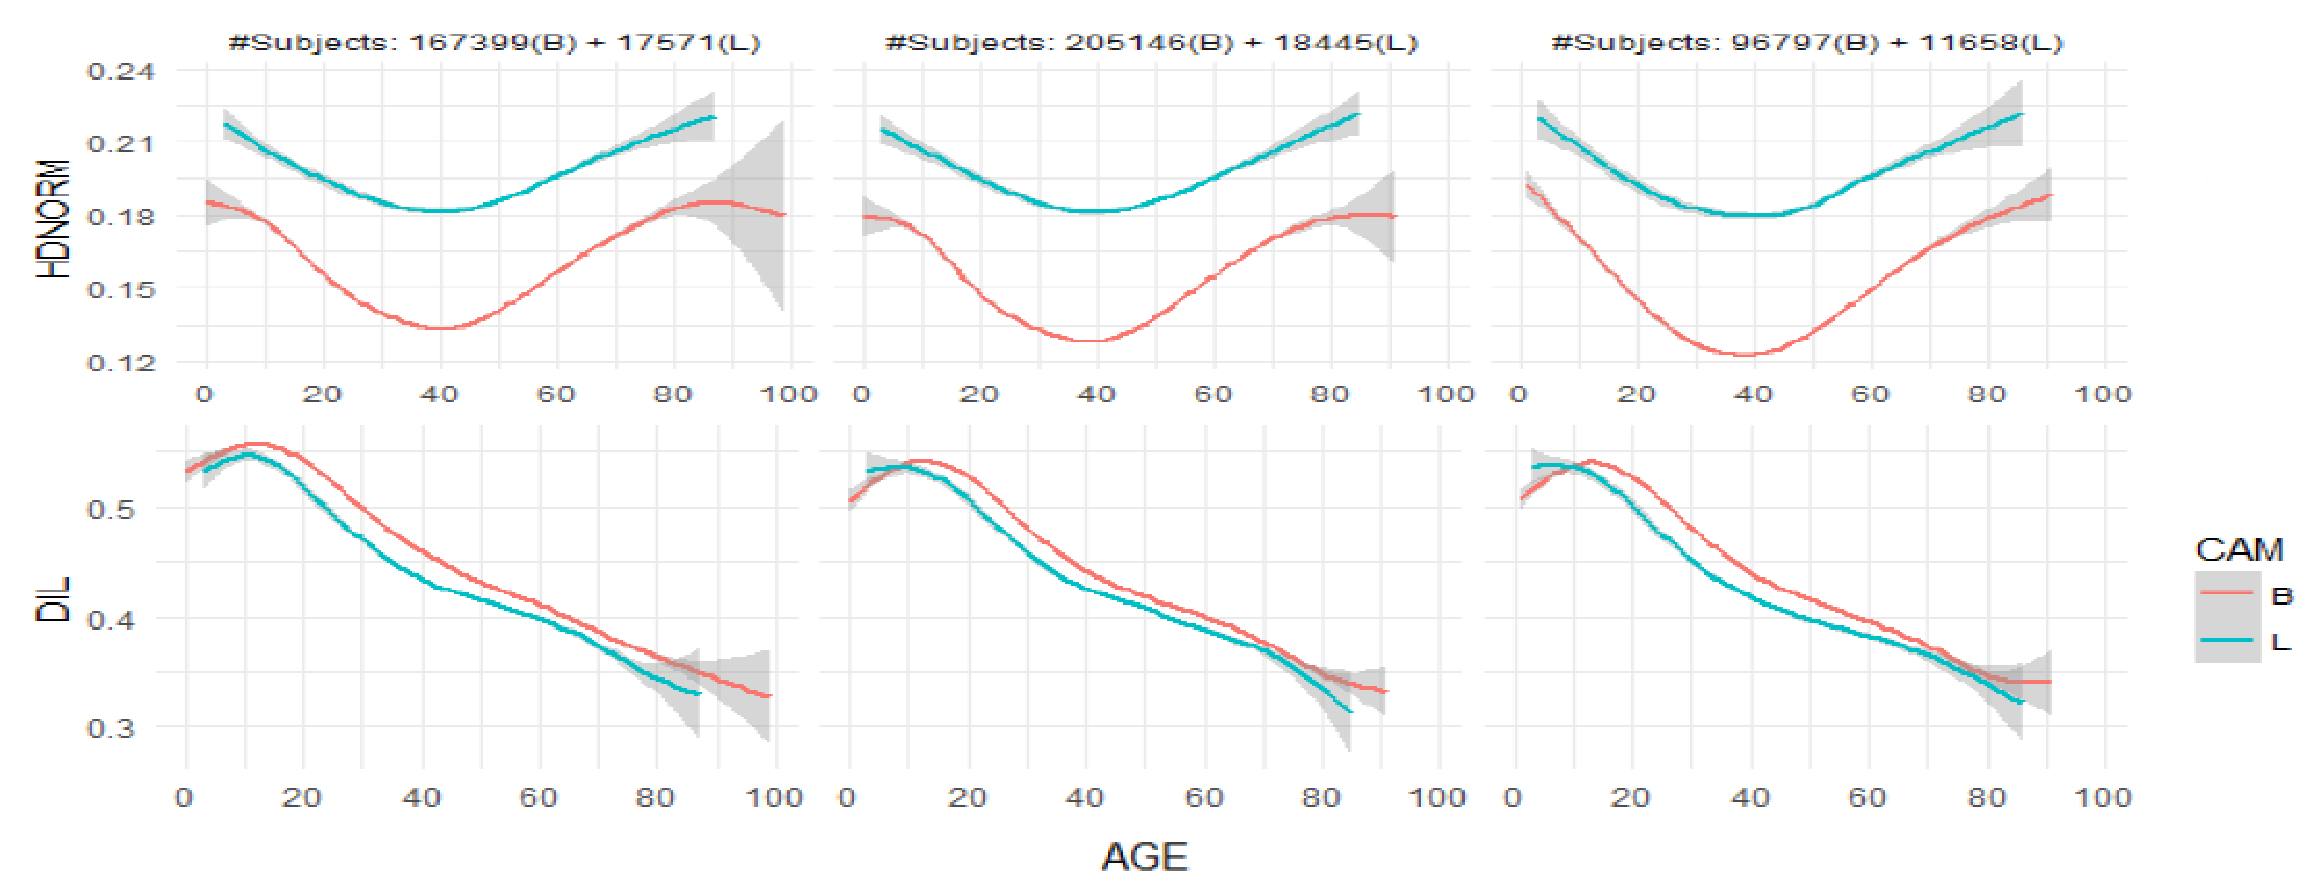
\includegraphics[width=0.49\linewidth,height=2.2in]{eps/1-ALL=f(AGE)-2.eps} 
b)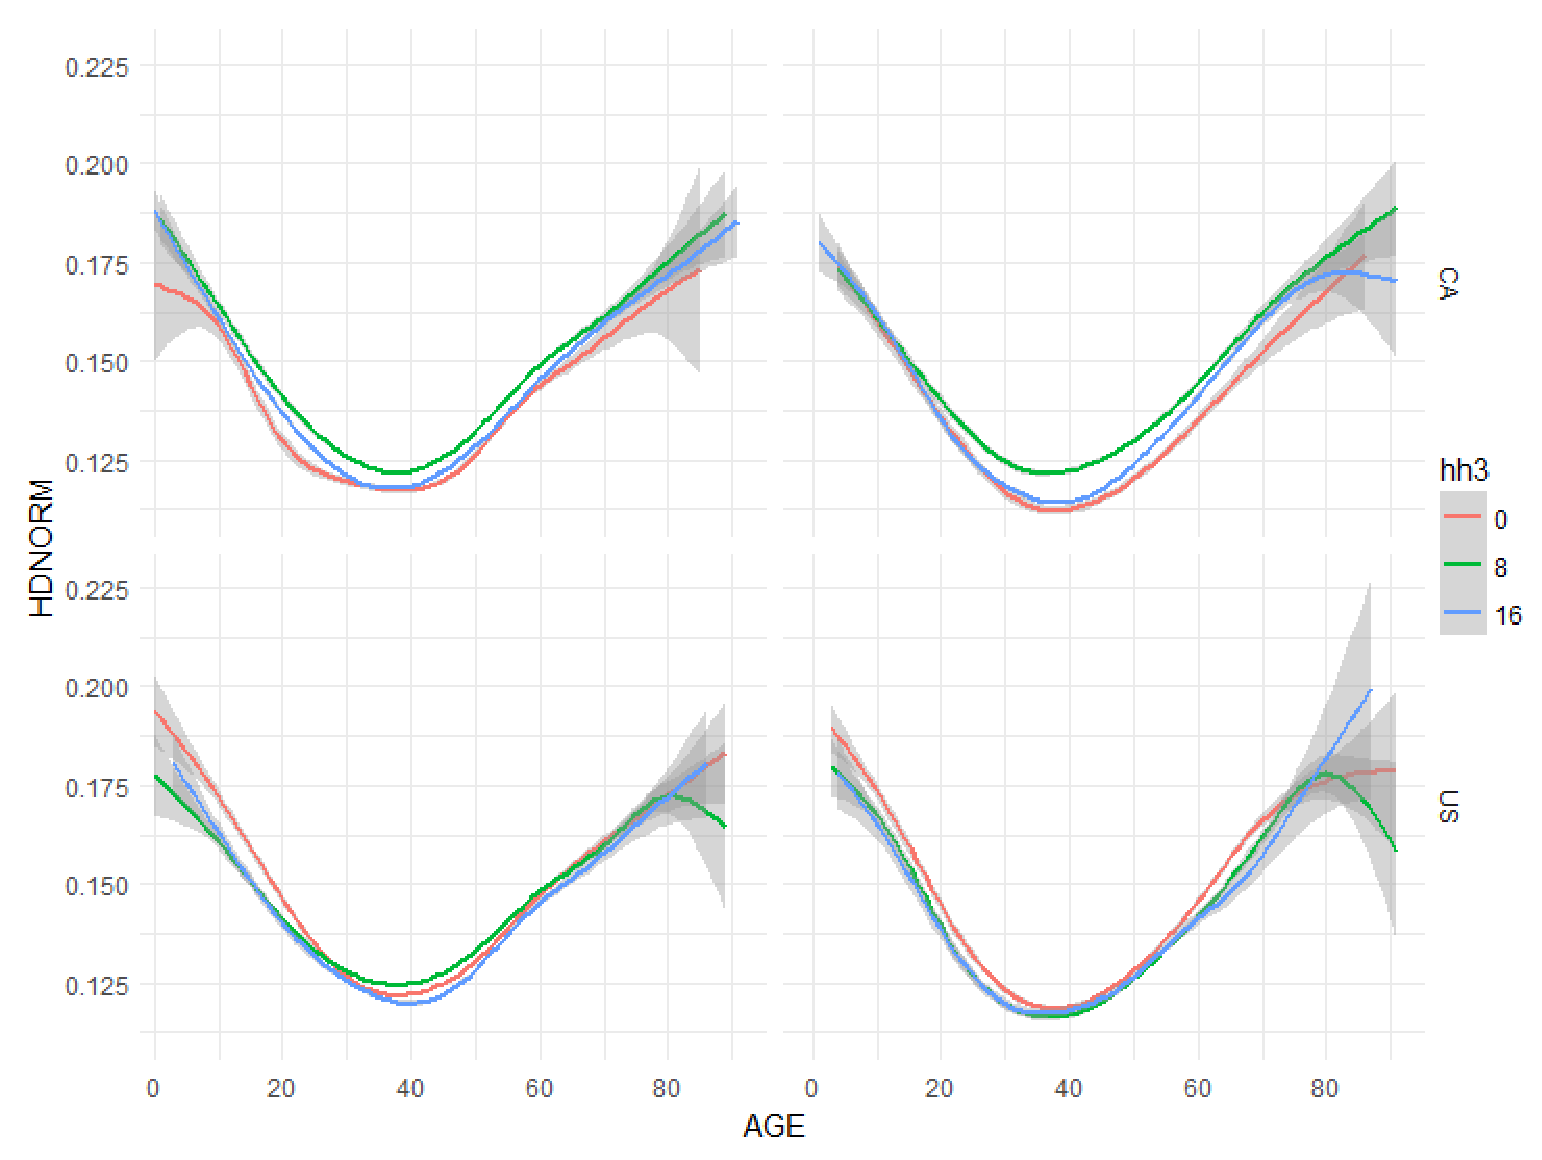
\includegraphics[width=0.45\linewidth,height=2.2in]{eps/1M-hh3-best.eps} 
%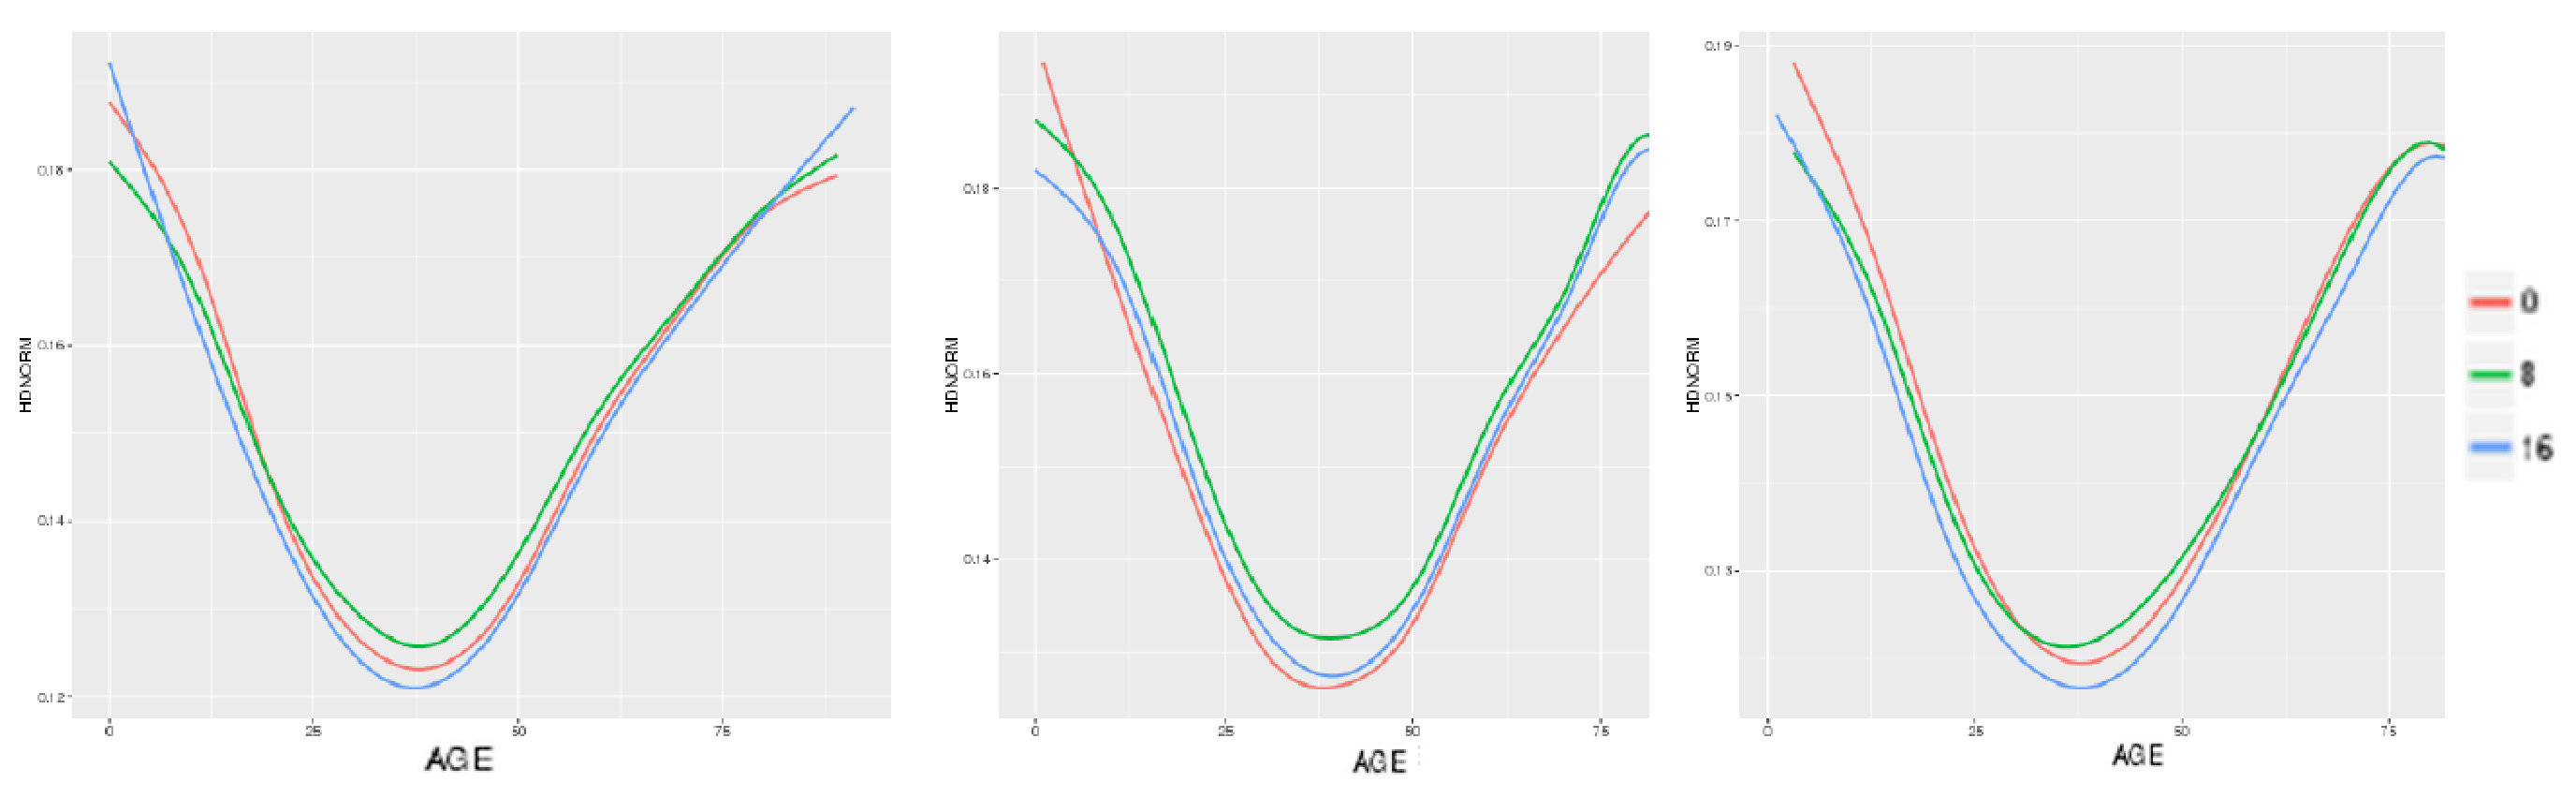
\includegraphics[width=0.49\linewidth,height=2.0in]{eps/HDNORM=f(AGE,hh)8-ABD.eps}

%\caption{ Effect of age vs. time of day at three airports:  average HDNORM computed using generalized additive model regression  for three time intervals (0:00-8:00 in red, 8:00-16:00 in green, 16:00-24:00 in blue).
%%: clockwise – Toronto T1, Vancouver, Calgary and Montreal. 
%and average Transactions Per Subject ($T/S$) ratio,
	
	
\caption{
Effect of age. 
%Effect of age  at three airports: 
%a) The number of transactions per subject  for each age group at each airport; 
\figfooter{a} { Average HDNORM and DIL computed 
for subjects enrolled with old (`L') and new (`B') cameras at three largest airports
using generalized additive models (gam) regression. 
%using generalized additive models (gam) regression. 
}
\figfooter{b} {  Average HDNORM  computed for subjects enrolled with new (`B') cameras at different times of day: 0:00-8:00 (in red), 8:00-16:00 (in green), 16:00-24:00 (in blue). 
%Left-eye transactions   in two large airports are used.
%Subject-based metrics are used. 
%Analysis is conducted using subject-based metrics. 
%Averages are computed using generalized additive model regression. 
%, using data from three largest airports  (Toronto T1, Vancouver, and Montreal.) 
}
\label{fAGEvsTime}}
\end{figure*}



\begin{figure*} [!b] 
\centering
%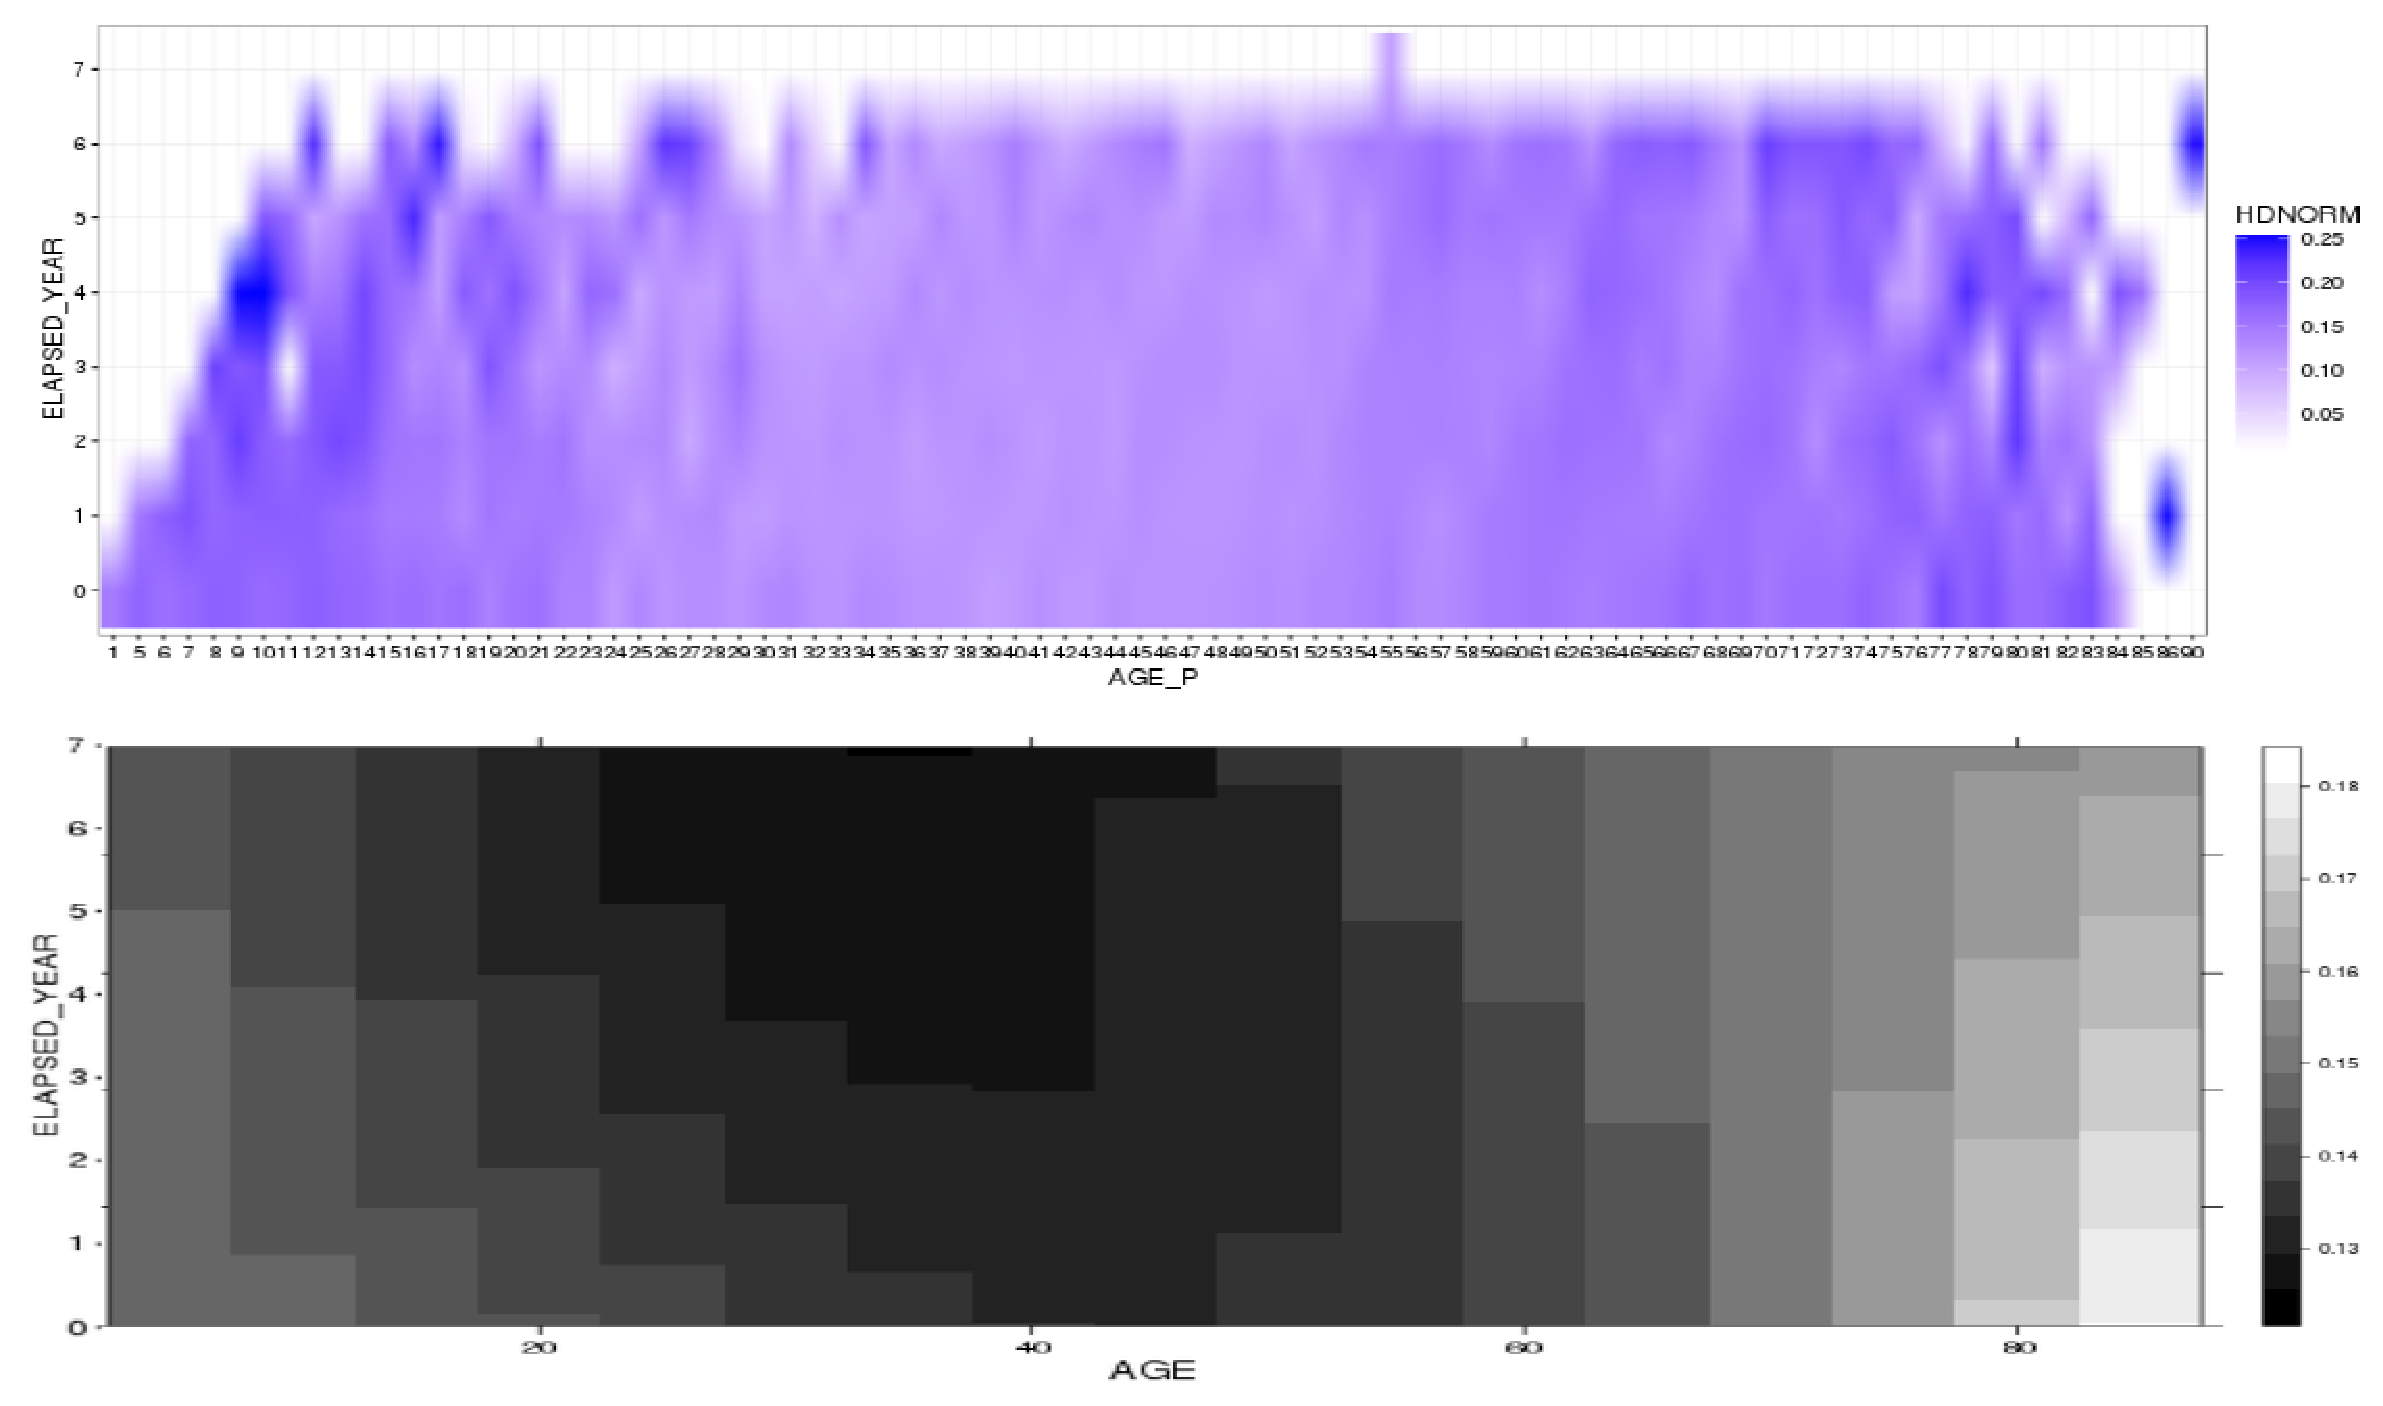
\includegraphics[width=0.5\linewidth,height=1.8in]{eps/heatmap-both.eps}
%a) 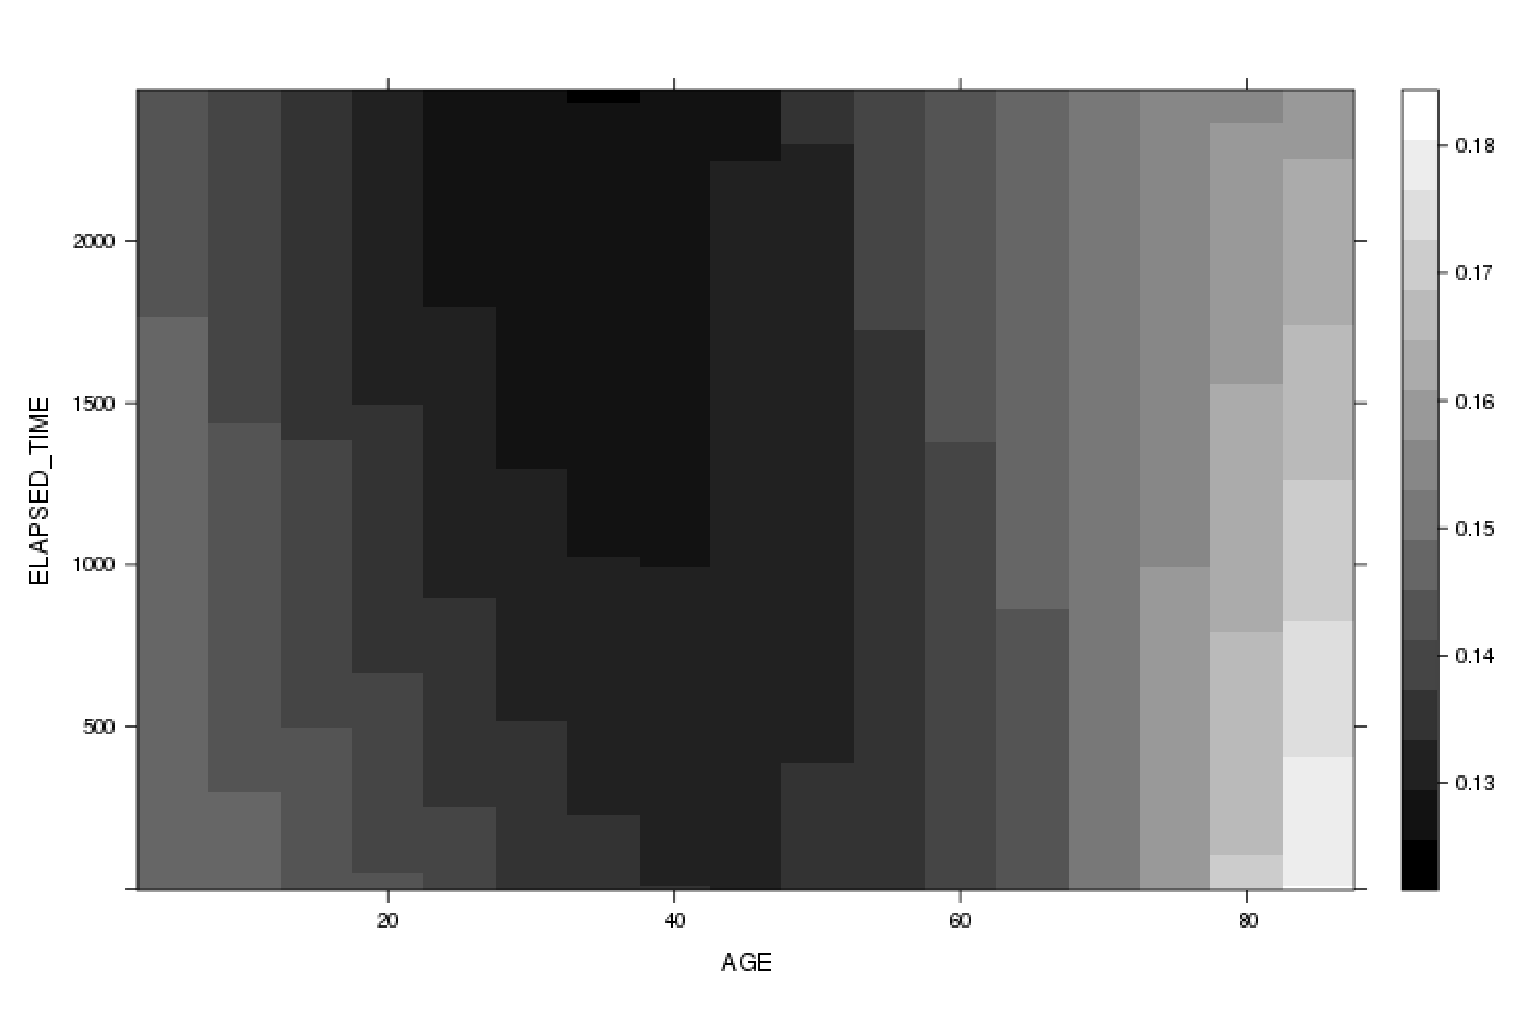
\includegraphics[width=0.5\linewidth,height=1.8in]{eps/HDRawvsAGE-ELAPSED(example).eps} \quad 
a)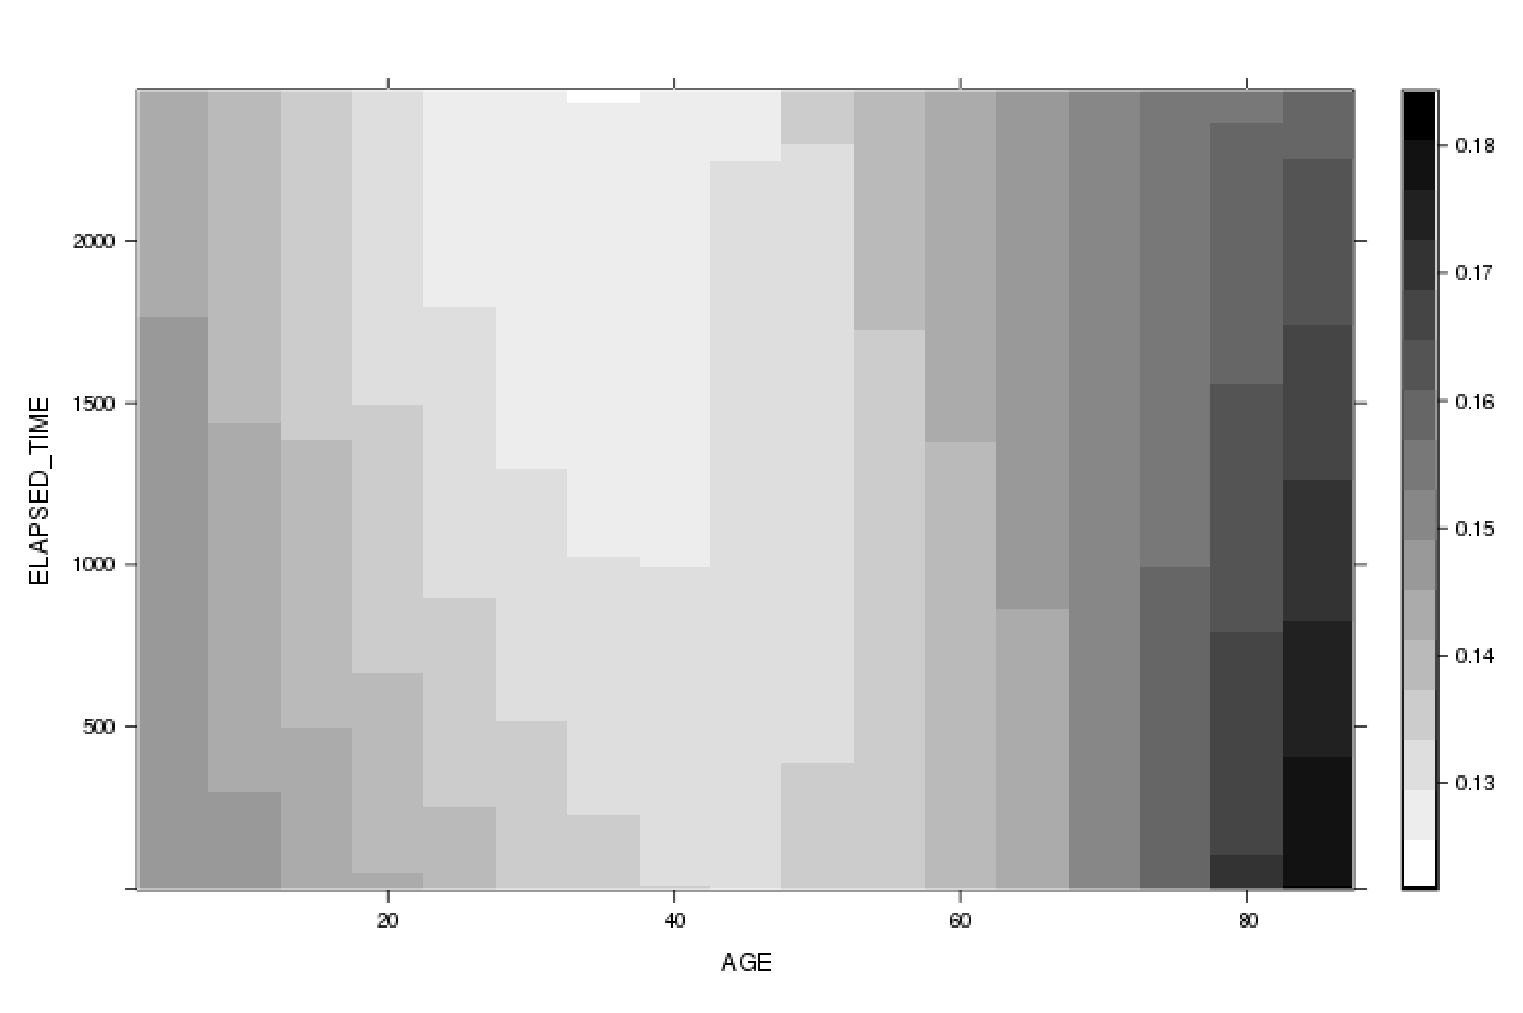
\includegraphics[width=0.5\linewidth,height=1in]{eps/HDNORMvsAGE-ELAPSED(inverted).eps}  
%\includegraphics[width=\linewidth,height=1in]{eps/heatmap-year-interpolated.eps} \ \ 
%\includegraphics[width=\linewidth, height=1in]{eps/heatmap-year-GAM.eps} 
%%\includegraphics[width=0.95\linewidth,height=1in]{eps/HD=f(age,EL).eps} 
%%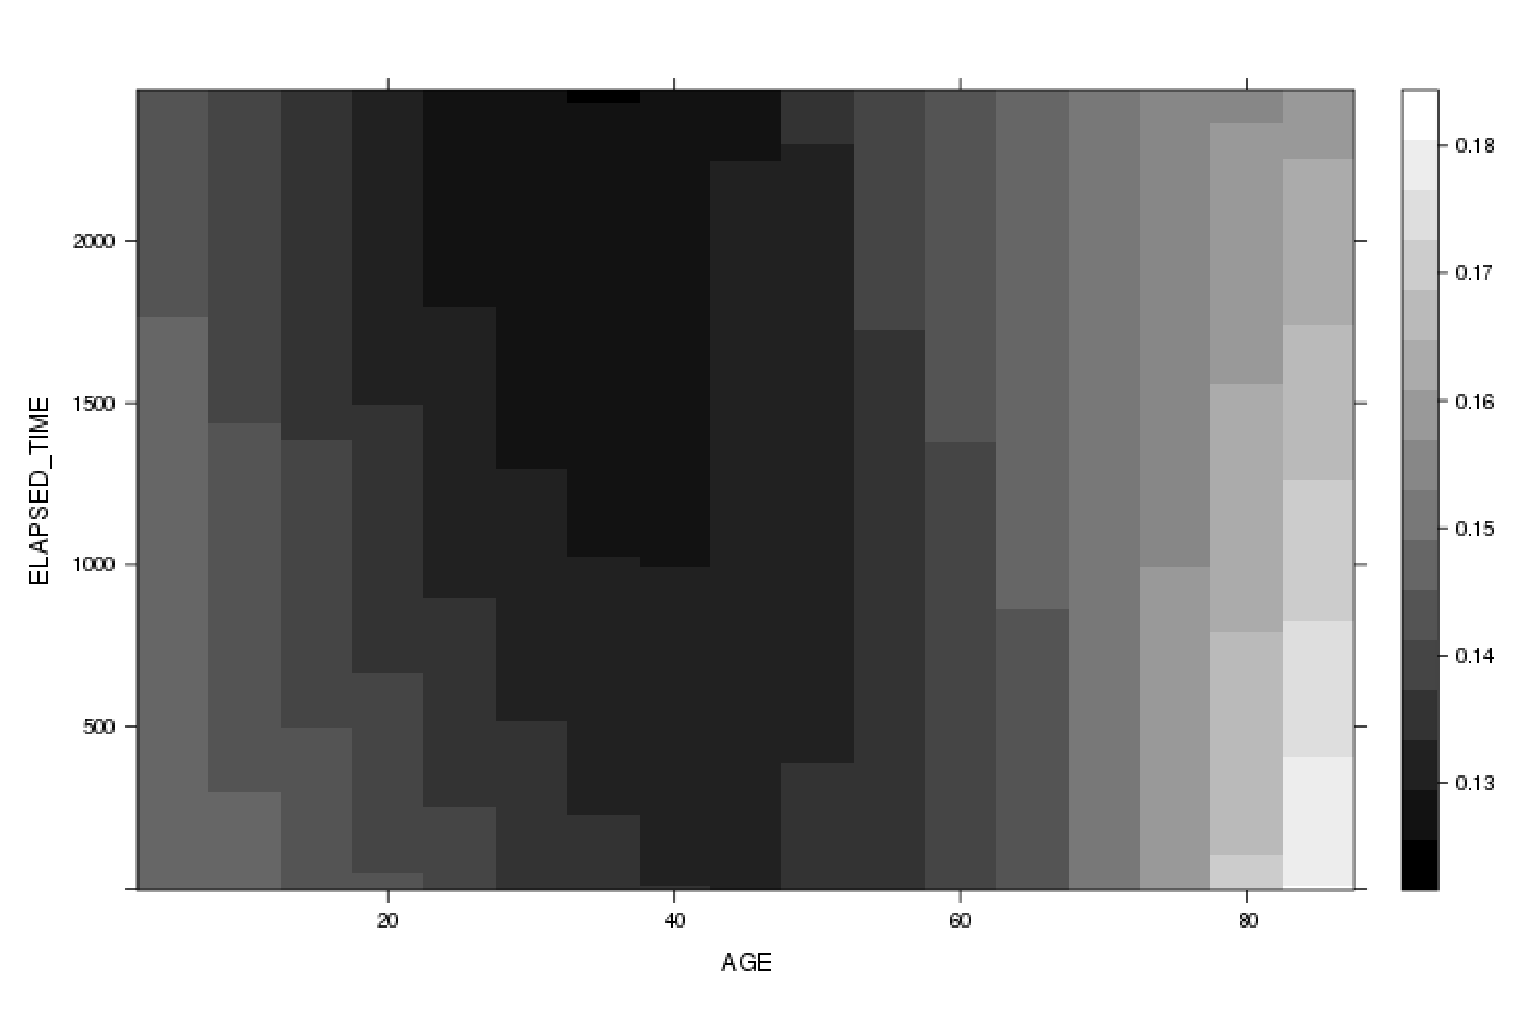
\includegraphics[width=0.95\linewidth, height=1in]{eps/HDRawvsAGE-ELAPSED(example).eps} 
% HDRawvsAGE-ELAPSED(example).eps} 
%\label{fAgeAging}
%\end{figure}
%\vspace{5pt}\hrule\vspace{6pt}
b)
%\begin{figure} [!b] 
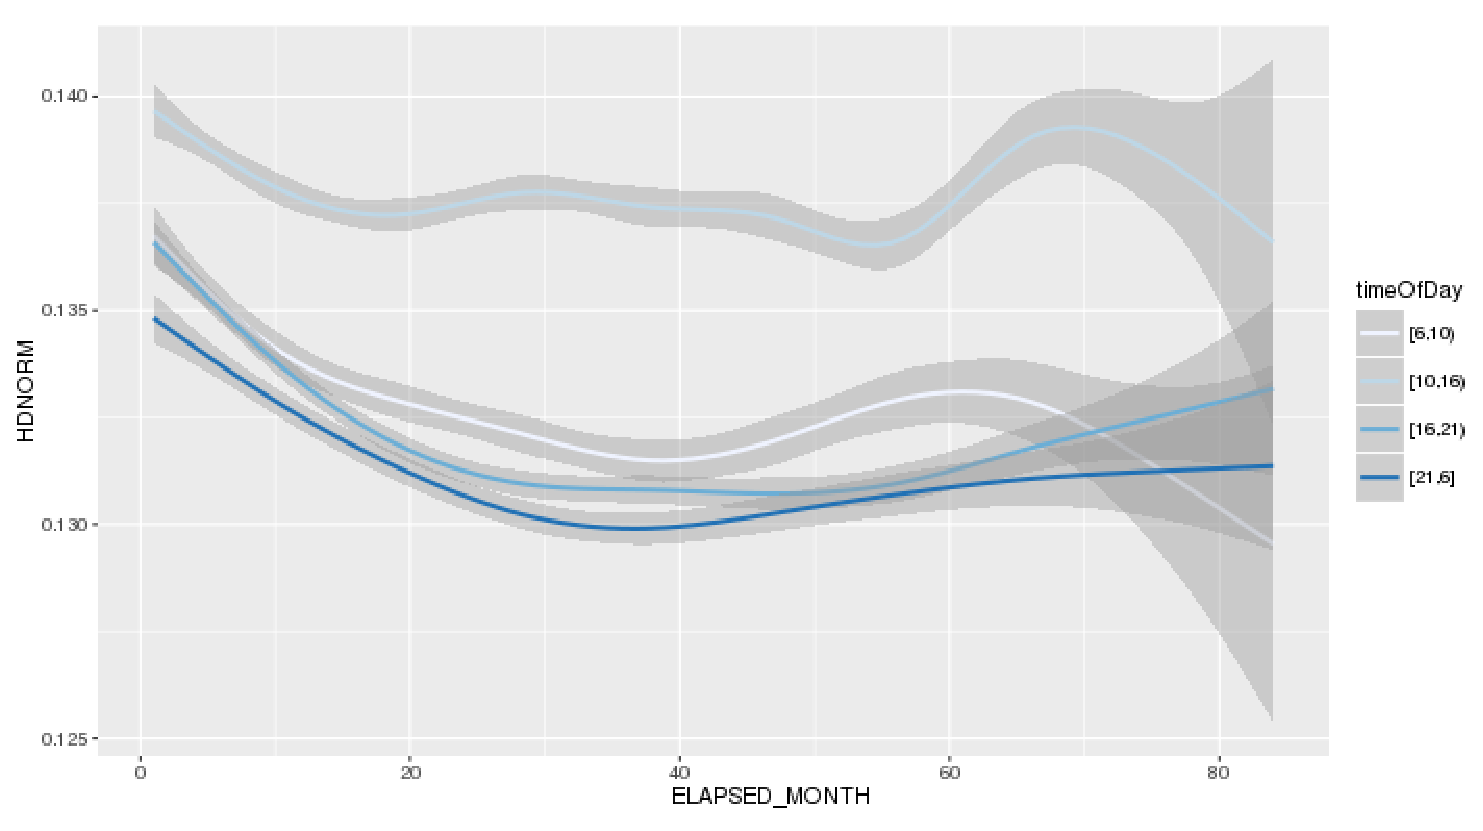
\includegraphics[width=0.45\linewidth,height=1in]{eps/HDNORM=F(ELAPSE,hh)-PORT=A.eps} 

%\caption{Effect of age vs. aging: HDRAW as a function of Age and Aging -- heatmap of raw values (top) and computed using generalized additive model least-square regression (bottom). }
\caption{Effect of aging. 
%Analysis is done on Left-eye passage transactions for travellers enrolled with new (`B') cameras.
%Variation of HDNORM by Aging vs. age and time of day: 
\figfooter{a} { 
Average HDRAW as a function of AGE and the number of days since enrollment (ELAPSED\_TIME) computed using generalized additive mixed models (gamm) regression.  
Kiosk fake id (FAKE\_KIOSK\_ID) and traveller's fake id (FAKE\_ID) are treated as random effects, while AGE and ELAPSED\_TIME are treated as fixed effects.
%  using data from all Passage kiosks.
%Average HDNORM scores mapped on two-dimensional `age'-`aging' space, where each cell  corresponds to a unique age group (AGE) and number of years since enrollment (ELAPSED\_YEAR). The top image shows score average for each group. The bottom image shows  score averages extrapolated using generalized additive model regression. 
%The darker the cell, the worse the matching score. Data from all kiosks is used.
}
\figfooter{b} {  Average HDNORM as a function of the number of months since enrollment (ELAPSED\_MONTH) computed  using generalized additive model (gam) regression  at different times of day of the passage. Data from a single airport, where variation due to kiosk location is small, are used.
%Data  all kiosks in a single airport are used. %in Port A (Toronto T1).
}
\label{fAgingHH}}
\end{figure*}



%\subsection{Variation by age vs. kiosk location }
%\subsection{Variation by age vs. kiosk location }


Figure \ref{fAGEvsTime}-a %fAGEvsKIOSK} 
%shows the average HDNORM and  DIL scores computed using generalized additive model  regression
plots the average HDNORM and  DIL scores as a function of AGE computed using generalized additive model (gam) regression
%Figure \ref{fAGEvsKIOSK} shows  HDNORM as a function of age computed using least-square regression 
\cite{R-book} for   three largest Canadian airports (Toronto Terminal~1, Vancouver, and Montreal).
Subject-based analysis is conducted separately for each airport for travellers enrolled with old (`L') and new (`B') cameras.
The number of subjects at each airports for each camera is indicated on the top of which graph.
The gray area shows 95\% confidence interval. 
Large gray areas for travellers of over 80 years of age indicate that there is no sufficient data to reliably compute the function.

A clear drop in average matching scores (i.e., better performance) for middle-aged travellers is observed at each airport: from 0.18 (for those younger than 15 years  and older than 80 years) to less than 0.14 for 40-year old travellers.
This is in contrast to average Dilation, which monotonically decreases with age: from 0.55 (at 15 years of age)  to 0.35 (at 80 years of age).
This is an indication that Dilation is \textit{not} the only factor that contributes to worsening of the matching score. 
Other Image Quality metrics are also likely affecting the result.

%In order to minimize the effect due to being in a different airport, %which is shown above affects the technology performance, only the data from three largest Canadian airports (Toronto Terminal 1, Vancouver, and Montreal) are considered only.% and compared to each other.
It is also noted that kiosks in Vancouver airport have been relocated during the period of data collection, resulting  in their improved performance (which was noted in \cite{Bowyer-BTAS2016}). This however did not affect the result related to the variation of system performance by age.
It is also seen that variation due to age  is larger than that due to kiosk location.


%Finally, to address the concerns related to the use of iris biometrics by minors, as done in  humanitarian and national ID programs %\cite{FBI-IJCB2014},
%Finally, to address the high interest in using iris biometrics for humanitarian and national ID programs \cite{FBI-IJCB2014},
%to address concerns related to the use of iris biometrics with young children for humanitarian and national ID programs \cite{FBI-IJCB2014},
%knowing the high interest in using iris biometrics for humanitarian and national ID programs \cite{FBI-IJCB2014}, 
%we can note that,
% based on the obtained results, it can be stated that
%(from  our Enrollment and Passage age statistics)  
% iris biometrics is as successfully used by  children (less than 15 years old) and youth as it by elderly.
%the performance of the technology with  young children (15 years old) is comparable to that with elderly (over 70 years old). 





\subsection{Age vs. time of day and time of year}

%Variation of system performance by time of day has been noted in \cite{Bowyer-BTAS2016}. To further examine this effect and to compare it to that of age, 
%To compare this effect to that of age, we


The data used  in the previous experiment is further split into three subsets, corresponding to three different times of day (morning, mid-day, evening), using Left-eye transaction data from travellers enrolled with  `B' cameras.
Figure \ref{fAGEvsTime}-b shows the results for two airports.  
Bottom row shows results for kiosks in US pre-clearance area, top row for kiosks in the arrival area.




%The data used  in the previous experiment is further split into three subsets for each airport, corresponding to three different times of day (morning, mid-day, evening).  Figure \ref{fAGEvsTime}-b shows the results. The data from travellers enrolled with new `B` cameras are used. 
%Note that the scales in vertical axes are different for each airport in this figure.

%Figure \ref{fAGEvsTime} shows  average HDNORM as a function of age computed using GAM regression at three largest airports (Toronto Terminal 1, Vancouver, and Montreal)  at three different times of day (morning, mid-day, evening).  

A  slight  increase in matching scores for all ages at mid-day, i.e., during the brightest time of the day, is seen in two areas. 
%This is consistent with earlier knowledge that iris sensors work worse in daylight 
This is consistent with earlier results suggesting that iris recognition produces poorer match scores when passage image acquisition takes place in strong sunlight, 
and is an indication that kiosks in those two airports are likely located where a large amount of sunlight comes through the windows.
Critically however, it is seen that  performance variation due to day time difference is much less than that due to age difference.
%this increase is much  

%As  reported in \cite{Bowyer-BTAS2016}, 
In another experiment, some consistent increase in HDNORM during December - January was also observed,  supporting  earlier such funding in \cite{Bowyer-BTAS2016}. 
In contrast to \cite{Bowyer-BTAS2016} however, where such variation is explained by the effect of season on eye dilation, 
%where the effect of season on eye dilation is suggested to explain the phenomenon, 
we are inclined to think that   most likely this is due to the subject-based performance variation, 
%since it is during the holiday seasons when people who rarely use the system use it.
%This can be explained by the subject-based performance variation, 
as more people travel and use the technology during the holiday season, including those who do not travel often and who (based on the results presented above) have a higher risk of experiencing the difficulty in using the system.  
In either case, the effect of  time of the year is also seen to be much less than that of age  and kiosk location.
%others discussed above.
%In either case, the effects of time of day and time of year appear to be of  much lesser scale than those due to age and kiosk location.

\subsection{Age vs. aging}

%With respect to aging debate between NIST and UND researchers ..
To address the debate between NIST and UND researchers related to the effect of aging, 
%which is the deterioration of performance with time,
we compare this effect to that of age and other factors.
In order to do that, we apply 
{\it generalized additive mixed models} (gamm) regression \cite{R-gam}
%to model HDNORM scores
to compute average HDRAW scores as a function of age (AGE) and aging (measured by the number of days since enrollment, ELAPSED\_TIME)
%measured by the number of years since enrollment ELAPSED\_YEAR)
using  Left-eye passage data from all kiosks for all users enrolled with `B' cameras.

In contrast to {\it generalized additive  models} (gam)  used earlier (Figure \ref{fAGEvsTime}), 
%https://stats.idre.ucla.edu/r/faq/how-can-i-explore-different-smooths-in-ggplot2/
%https://m-clark.github.io/docs/GAMS.pdf
{\it generalized additive mixed models} allow one to include random effects, which in this case are kiosk location (FAKE\_KIOSK\_ID) and person's physiology (FAKE\_ID), in addition to fixed effect (AGE and ELAPSED\_YEAR).
The `gamm' function from the `mgcv' R package is used for this purpose \cite{R-gam}.

\cmt{
Using the `mgcv` R package \cite{R-gam}, the relationship between the effects and the output value (HDRAW) is defined by the following 
formula:
{\scriptsize  
\begin{verbatim}  
model = gamm( HDRAW ~ te(ELAPSED_TIME, AGE), data=OPS_XING,
              random=list(FAKE_ID=~1, FAKE_KIOSK_ID=~1) ) 
\end{verbatim}
}

 %predData <- expand.grid(ELAPSE=seq(1,2506,100), AGE=seq(0,85,5))
 % pred <- predict(mdl$gam, newdata=predData, type="response")

In this formula,  {\tt te()} is used to  apply a tensor product smooth to obtain better smoothing for the function on the marginal values.
%(which provides better smoothing for the function on the marginal values)
%and {\tt family=Gamma} is used to allow a larger variety of functions to be applied in smoothing. 
}

Once the predictive model is computed, it is applied to compute the  expected average HDRAW scores for a grid of age-aging values,  where age is incremented by 5 years, and aging (ELAPSED\_TIME) by 100 days. The result 
%of thus obtained heatmap of average HDNRAW scores for different AGE and ELAPSED\_TIME values 
is shown in Figure~\ref{fAgingHH}-a.
The following  observations are made.

\cmt{
%shows the  heatmap of  HDNORM scores for different Age at Passage (AGE\_P) and different number of years since enrollment (ELAPSED\_YEAR).
shows the  heatmap of  HDNORM scores for different Age at Passage  and different number of years since enrollment (ELAPSED\_YEAR).
The top image shows interpolated (i.e., averaged between adjacent bins) mathematical average of HDNORM for each `age'-`aging' group. 
The bottom image shows average  HDNORM scores for different Age and ELAPSED\_YEAR computed using generalized additive model regression. Data from all kiosks and all cameras are used. 
% and computed using subject-based metrics  

}
%Low HDNORM values are shown in light blue, high HDNORM values are shown in dark blue. The interpolated data is shown (i.e., averaged between adjacent bins).

%By visually examining the variation of heatmap colour , we note that variation due to Age is larger than that due to Aging (ELAPSED\_YEAR). 

%Then, we apply GAM regression to compute the average  HDNORM scores for different Ageand Aging (ELAPSED\_YEAR) bins.
%The result is shown in Figure \ref{fAgingHH}-b. Low HDNORM values are shown in black, high HDNORM values are shown in white.



First, for all ELAPSED\_TIME groups (i.e., along the horizontal axis), 
the relationship between the matching score and age is exactly the same as found earlier (seen in Figure \ref{fAGEvsTime}):
the matching score is the lowest at 35-40 years of age and monotonically increases as one moves further away (left or right) from the middle. %with largest va due to age difference being 0.05

Second, for most age groups (i.e., along the vertical axis), aging has no negative effect on matching scores. 
%confirming the results reported in \cite{irexVI,aging3}. 
It is only for 55-65 age group, where slightly increased (worse) matching scores with aging are observed.
Critically, the variation in matching score due to aging is much less than that due to age difference.

\cmt{
No increase of HDRAW with ELAPSED\_TIME (i.e., along the vertical axis) for either age group is observed, which 
confirms results reported in \cite{irexVI,aging3}.
 However,  an increase of HDNORM with Age (i.e., along the horizontal axis) for travellers over 40 years of age is observed.
 }

%As an explanation of the observed improvement of HDNORM score with ELAPSED\_TIME, we provide the following three reasons:  
%The observed decrease (improvement) of HDNORM score with ELAPSED\_YEAR for each age group can be explained by several factors:
 %1) habituation (travellers learn how to make the machine work better for them, e.g., by opening wider their eyes), 2) the improved positioning of the kiosks (as in Vancouver, found in \cite{Bowyer-BTAS2016}),  and 3) the use of transaction-based metrics (which show `better' results for travellers who use the system more often). 
%urther 

To explain the observed improvement of HDNORM score with ELAPSED\_TIME, we offer the following four reasons: 1) habituation (travellers learn how to make the machine work better for them, e.g., by opening wider their eyes), 2) the improved positioning of the kiosks (as in Vancouver, found in \cite{Bowyer-BTAS2016}), and 3) the use of transaction-based metrics (which show `better' results for travellers who use the system more often), and 4) the reduction over time in the threshold for recording a match score, THD, means that subjects who use the system over a period of years are able to record a higher score in the earlier years of using the system than they are able to record in the later years.


%Ottawa airport (at arrival and departure combined).



%\subsection{Aging vs. time of day}

In order to further quantity the \cmt {negligible} effect of Aging, we compare it to that of 
time of day. Figure~\ref{fAgingHH}-b shows the average HDNORM computed using generalized additive model regression on the data taken from a single airport (which has little variation among its kiosks) as a function of Aging (ELAPSED\_MONTH) for four different times of day (morning, mid-day, evening and night).
It is observed that the effect of aging is less  than that of time of day of passage transaction, which in turn (as discussed earlier) is less than the effect of age and kiosk location.

To conclude, 
taking into account the results from previous sections, where it was shown that age correlates with IQ metrics, particularly, with Dilation  and (to lesser degree) with Contrast, it can be stated 
%(as was first done in the “ART in ABC” study [1-2])  
that ``aging problem'' is not about ``whether a biometrics modality changes in time'' (yes, it does), but rather about ``whether the technology can deal with the changes due to aging''. 
Evidently, iris biometrics can deal with changes due to aging quite well, at least 
over the range of years analyzed in this  study (which is seven years). 
At the same time, 
%as shown in this work 
it is seen that, as with all other biometric modalities, its performance is affected by sensor quality, capture conditions (lighting), and also by person's age (when comparing technology performance for  travellers of  different age groups).

%As highlighted in our report \cite{},  This makes iris modality most suitable
%In comparison, face recognition technology. 
%, which is not true compared, for example, to face recognition technology. % that cannot, at least at the present time. 



\begin{table}[!b]
%\processtable{The result of  the analysis of variance: confidence levels for factors and their combination. Results are shown from  kiosks in one airport.\label{fAOV}}
\caption{Analysis of variance in matching scores due to various factors. \label{fAOV}}
{
%Data are taken from kiosks in a single airport) }
%pa11 = pa[PORT=="G" & MODE == "SEM" & EYES==2 & D_yd==0] 
% D_yd is the difference in left and right eye enrollment dates
%aov.out=aov(HDNORM ~ oAGE*ELAPSED_YEAR + timeOfYear*timeOfDay, pa[PORT=="G" & MODE == "SEM" & EYES==2])
%summary(aov.out)
\tiny
\begin{verbatim}
                     Df Sum Sq.Mean Sq.F value        Pr(>F)   
AGE                   8  16  2.015 476.87 < 0.0000000000000002 ***
ELAPSED_YEAR          7   0  0.024   5.76         0.0000010803 ***
timeOfYear            3   0  0.043  10.07         0.0000012431 ***
timeOfDay             3   1  0.257  60.91 < 0.0000000000000002 ***
AGE:ELAPSED_YEAR     46   0  0.007   1.73               0.0015 **
timeOfYear:timeOfDay  9   0  0.026   6.19         0.0000000091 ***
\end{verbatim}
}
%Residuals       134512 568 0.004                                
{\scriptsize
Note: 
%Data from kiosks in a single airport are used.
The last column shows the probability $Pr(>F)$  of having the same mean output  value despite the change in input factor value. 
%All factors and their combinations are seen as being highly ($>99.9\%$) significant.
%, i.e. having $Pr(>F)$ close to zero.
}
\end{table}
%---
%Signif. codes:  0 *** 0.001 ** 0.01 * 0.05 . 0.1 


\begin{figure} [!t] \centering
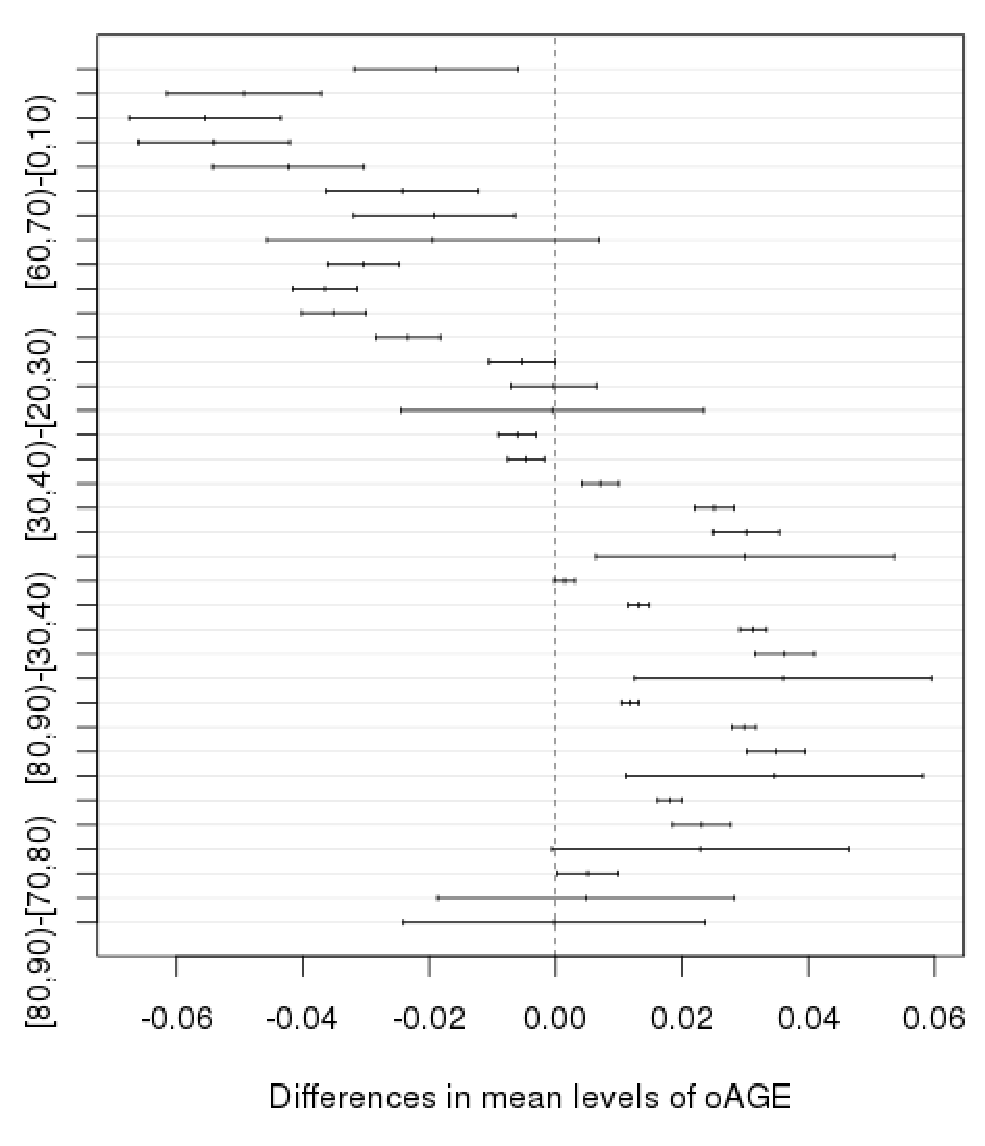
\includegraphics[width=0.5\linewidth,height=1.8in]{eps/PortG-aov-HDNORM=f(AGE,ELAPSE,yd,hh)-1-AGE-c.eps}%
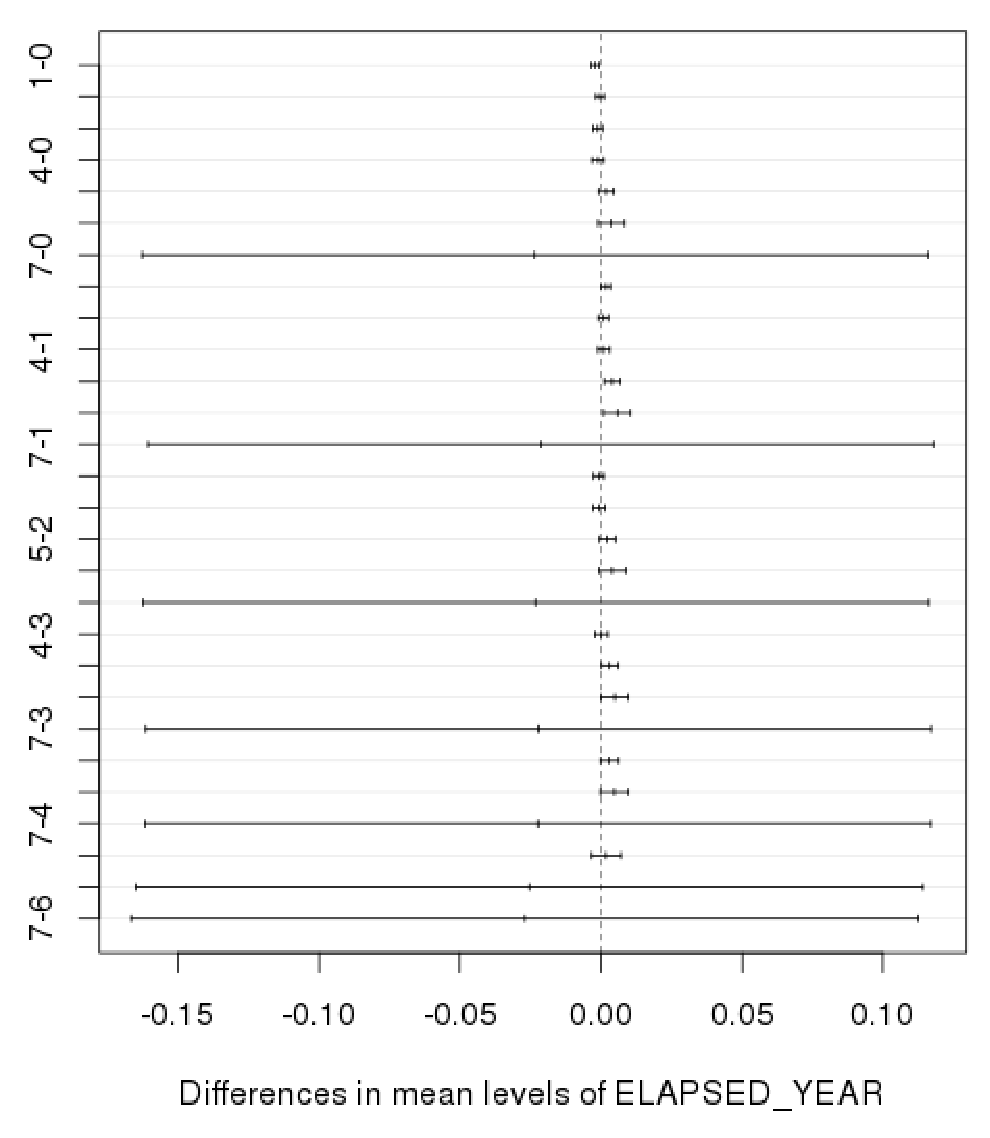
\includegraphics[width=0.5\linewidth,height=1.8in]{eps/PortG-aov-HDNORM=f(AGE,ELAPSE,yd,hh)-2ELAPSE-c.eps}\\
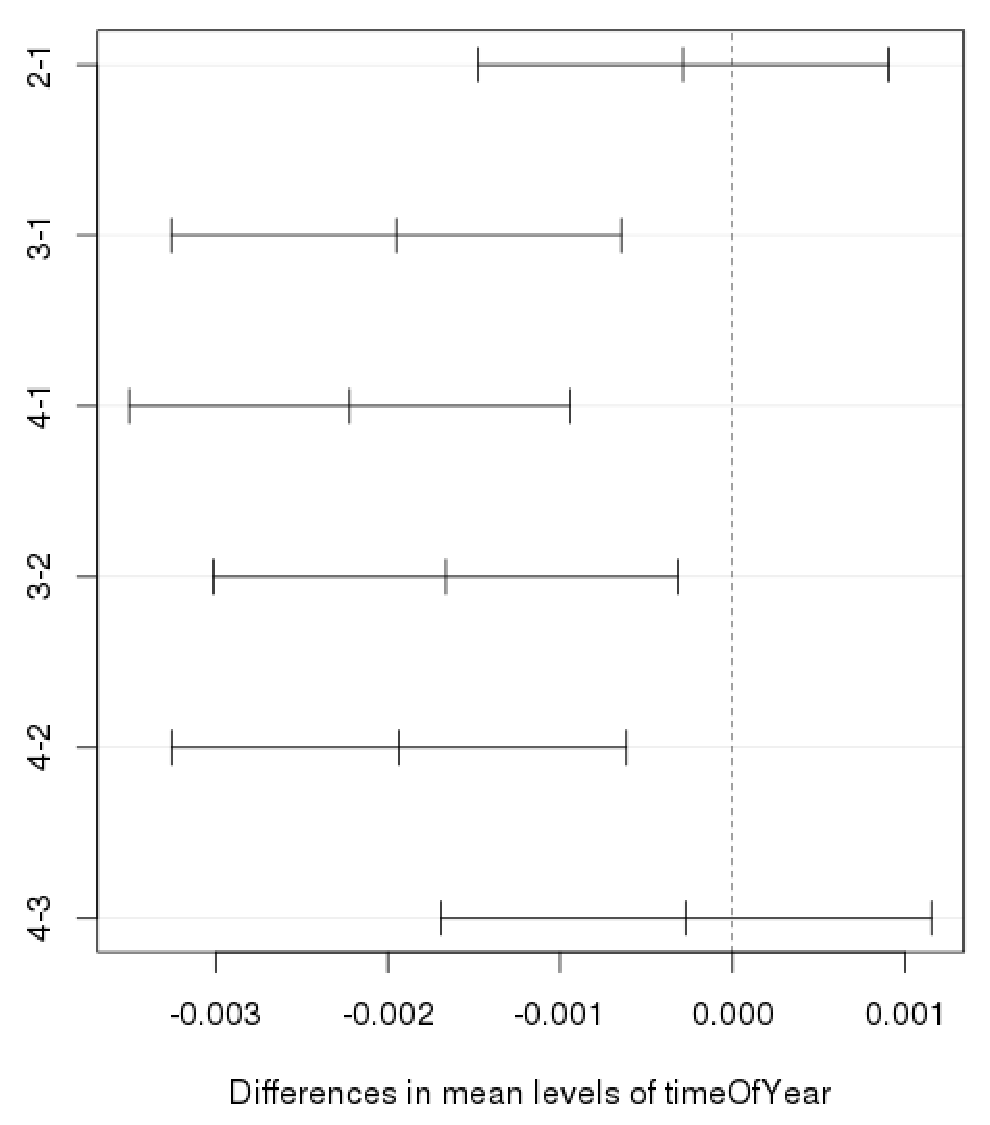
\includegraphics[width=0.5\linewidth,height=1.8in]{eps/PortG-aov-HDNORM=f(AGE,ELAPSE,yd,hh)-3Yd-c}%
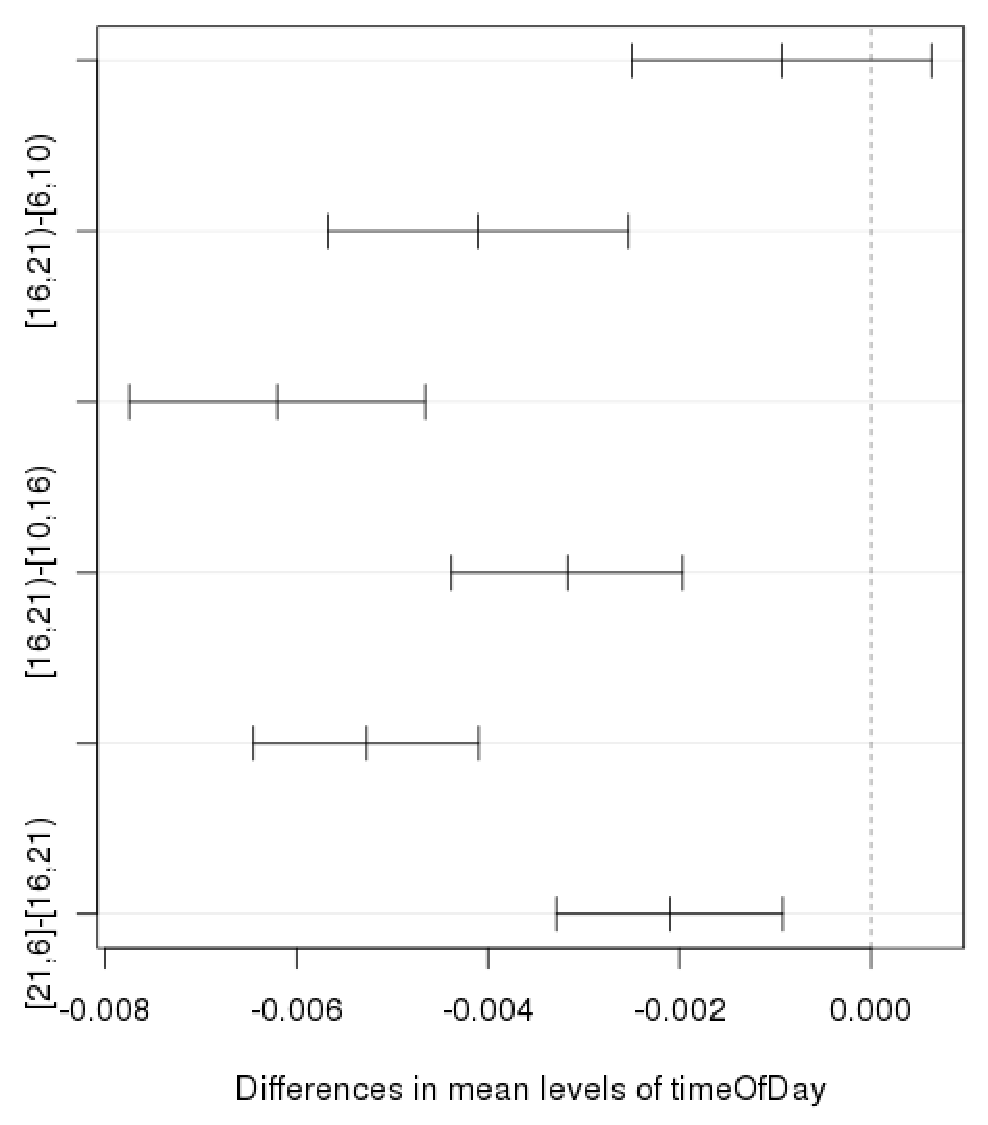
\includegraphics[width=0.5\linewidth,height=1.8in]{eps/PortG-aov-HDNORM=f(AGE,ELAPSE,yd,hh)-4-hh-c}

\caption{
%Analysis of variance of matching score: the 95\% confidence levels for four factors: age, aging, time of day and time of year. 
%Data are taken for kiosks in Ottawa airport (at arrival and departure combined).
The 95\%  confidence level intervals on matching score difference for all pair-wise value combinations of four factors:  clockwise --  age (9-level factor), aging (8-level factor), time of day (4-level factor) and time of year (4-level factor). %comparisons of factors values combinations 
}

\label{fAOVplots}

\end{figure}



\subsection{Factor significance}

Once the effect of certain factors (explanatory variables) on the performance of the system (response variables) is hypothesized through the observations of descriptive statistics (Figures~\ref{fAGEvsTime}-\ref{fAgingHH}), it is possible to apply analysis of variance  to 
obtain the values of statistical significance for each factor and their combination \cite{R-book}.
This is done below, where 
a combination of subject-related (age), technology-related (aging), and process-related (time of day and time of year) factors are examined for statistical significance.
 
To avoid the variation due to kiosk location, the data from kiosks in a single airport (where variation due to kiosk location is small) are used. Age is presented as 9-level factor (each level representing a decade), aging is 8-level  factor (each level representing a year since enrollment), time of day and time of year are presented as 4-level factors (as done in previous sections).
%(at arrival and departure combined).
Table \ref{fAOV} shows the result, as produced by running the analysis of variance in R language \cite{R-book}.
%shows the confidence intervals for each factor values and derived thereon.
%The factors and their combination that contribute to the variation in system performance with high ($>99.9\%$) significance are marked with (***). 
%The plots showing 95\% \cmt{factor-wise} confidence levels for all factor values combinations are shown in Figure \ref{fAOVplots}. 
%difference due to 
The plots showing 95\% \cmt{factor-wise} confidence level intervals on matching score differences for all pair-wise combinations of factors values %comparisons of factors values combinations 
are presented in Figure \ref{fAOVplots}. 


It is seen that all listed factors are statistically ($>99.9\%$) significant, 
with a combination of age and aging being  less significant than other factors. % or combination thereof).
%In this work we see that there are possibly many factors that affect the performance of iris technology. 
From a practical point of view however,
the important question is not which factors affect the technology performance but to what degree they affect it. 

Critically, for an organization  deploying the technology it is important to know  whether any action is required to improve the system performance. 
%the cost of which would
According to the ``technology-process-subject'' factor triangle (described in Section \ref{s.Factors}), three possible types of actions are possible: 
replacing the technology, improving the process, or implementing subject-based customization of the decision rules or procedures. 
As presented in the concluding section, the recommendations related to these actions appear visible from the results presented in this paper without the need of doing more detailed statistical analysis. 
%discussed in the conclusions


\section{Conclusions}



%When in early 2000
Iris biometrics was introduced to  automated border control as an extremely robust biometrics \cite{Daugman2002}.
% which rarely if ever produces errors.
%, extremely tolerant to external factors (compared to other modalities). 
%that produces errors with likelihood of ``tossing a coin heads up 249 times  in a row''  
Results obtained from a 
%examining  billions of matching scores from
watch-list screening border application in United Emirates \cite{Daugman2006} have  solidified this belief.
 %coining the expression to describe the likelihood of false recognition in iris biometrics as the likelihood of ``tossing a coin heads up 249 times  in a row''
%comparing the likelihood of false recognition in iris biometrics to that of ``tossing a coin heads up 249 times  in a row'' \cite{Daugman2006}.
%Not surprisingly, when later 
When later
the University of Notre Dame researchers 
%put under question one of the key tenets about this technology, 
published results showing that iris performance varied over time \cmt{ among the test participants} \cite{Bowyer,Bowyer2,Bowyer3}, it brought a lot of concern from the technology users, including many government organizations 
%such as DHS and CBSA 
who actively rely on iris technology in their operations \cite{aging}-\cite{aging3}. %, about the reliability of the technology.% and the ways it has been evaluated.
To address these concerns, NIST undertook an  effort
%and the largest to date effort  
to better understand the effect of aging and other factors on  iris biometrics \cite{irexVI}. 
This effort opened a whole new range of 
%other 
%questions related to the factors effecting the technology performance as well as the ways the iris biometrics performance is  evaluated \cite{Grother2015-iet}-\cite{Bowyer-BTAS2016}.
questions related to the factors that effect iris recognition
and  the ways  iris biometrics is  evaluated \cite{Grother2015-iet}-\cite{Bowyer-BTAS2016}.



Thanks to the efforts of NIST and UND scientists, our understanding about the properties and limitations of iris biometrics and current evaluation practices has improved significantly. The results presented in this paper further contribute to these efforts. 
Three major conclusions from the obtained results  are made.

First, in the applications where the use of technology is not mandatory,  as in automated border control \cite{GorodnichyARTinABC}, it should  be expected that subjects who experience problems using the system will use it less  than those who do not experience  problems. 
Hence, the performance of biometric systems in such applications, if  measured using traditional transaction-based metrics, may show unrealistic ``overly optimistic'' results. Therefore, the use of subject-based metrics introduced in this paper should be used when analyzing and reporting the performance of such systems. 


Second, in relationship to the aging debate \cite{IET0}, where the CBSA-collected OPS-XING dataset played a very important role, 
it is concluded that the effect of aging is negligible, compared to that of other factors such as kiosk location, time of day, and person's age.



While the effect of kiosk location and time of day on system performance has been  already uncovered by the UND researchers \cite{Bowyer-BTAS2016} using the previous releases of the OPS-XING dataset, the discovery of the effect of person's age on system performance was made possible only now, using the previously unused portions of the dataset.
It is shown that older (over 60 years  of age) and young (under 20 years of age) travellers are disadvantaged by the system. 
The system log shows  worse image quality and  matching scores for these groups, compared to that of middle-aged travellers. 
The variation of system performance due to age difference is larger than that due to light changes or different kiosk location.

In a society concerned with providing equal quality services to its all demographic groups (see \cite{GBA}), this finding may help to adjust its technology settings so that to mitigate  the demographic bias exhibited by the iris recognition technology. A new guidelines  document is being prepared by ISO in this regard \cite{ISO-bias}. 


To conclude, 
%From theoretical perspective, it may still possible to improve  the regression models 
it may still be possible theoretically to improve  the results of the analysis conducted on the OPS-XING dataset (e.g., by applying non-linear mixed-effect models \cite{R-book}).
% or apply more advanced statistical methods to  better describe the effect of various factors on the system performance, including the use of non-linear mixed-effect models or neural networks \cite{R-book-Zuur}, for example.
%or detect any new minor variotions of system performance due to a combination of already examined or not examined fac
% or analyze the effect of other factors that may potentially also affect the 
From practical perspective however, 
%as discussed in this paper, 
this additional effort appears of little importance, 
since none of analyzed factors appeared to effect significantly the system performance,
and
critical recommendations related to auditing and 
improving  iris recognition systems 
can  be made 
%to the organization deploying these systems, 
based on the results already obtained. 
These are listed below.
%, as presented in this paper.

Using the ``technology-process-subject'' factor categorization triangle, described in Section \ref{s.Factors}, 
the first 
%and most valuable 
step for improving iris recognition performance is seen in optimizing the kiosk placement (Process factor). 
%kiosk location is the variable in OPS-XING dataset that affected the number of additional requeried attempts the most.
%is the largelargest effect 
%to be correct placement of iris kiosks
%the prime caus
Then the performance can be further optimized by applying different matching decision or process rules for different age group populations (Subject factor). 
For example, 
a higher threshold or a larger number of attempts may be allowed for old and young subjects,
or  a score normalization formula can be further improved to take into account person's age and other image quality metrics, as discussed in Section \ref{s.NormRule}. This will mitigate the demographic bias exhibited by the system.
However, no action in relationship to aging-related concerns (Technology factor) appears to be needed.
%appears not to be required.

%It is however not possible  to conclude without a doubt that the observed age-dependent performance variation is due to the technology limitation, it may as well be due to the habituation phenomenon, because it is exactly the middle-aged users who used the technology the most.
%In either case, the affect of age, kiosk location and seasonal changes appear to be of one-two orders of magnitude larger than that of aging.

\cmt{
Then the performance can be further optimized by applying different matching decision or process rules for different age group populations, e.g., 
a higher threshold or a larger number of attempts for old and young subjects,
or matching score normalization formula can be further improved, as mentioned in this paper, to take into account person's age and other image quality metrics (Subject factor).
}




\section*{Acknowledgment}

This work was initiated and partially funded by the Canadian Safety and Security Program (CSSP) managed by the Defence Research and Development Canada,  Centre for Security Science (DRDC-CSS), as part of the CSSP-2013-CP-1020 (``ART in ABC'') project \cite{GorodnichyARTinABC} led by the CBSA. It has also contributed to the DRDC-funded CBSA-led CSSP-2015-TI-2158 (``Roadmap for Biometrics at the Border'') project deliverables related to the Gender-Based Analysis Plus (GBA+) \cite{GBA}.
%Its preliminary results are published in the project final report \cite{GorodnichyARTinABC}, and final results are presented in the internal report  ``Subject-based analysis of NEXUS iris recognition performance'', CBSA  Division Report 2016 – 12 (TR), August 2016.
%the “ART in ABC: Analysis of Risks and Trends in Automated Border Control” (D.O. Gorodnichy), Border Technology Division Report 2015 – 11 (TR), August 2015.
Feedback from  Kevin Bowyer, Adam Czajka,  Patrick Grother, and Jim Matey on iris technology related matters, and assistance from Jordan Pleet and 
%Rafael Kulik from University of Ottawa (on the statistical matters)
%hroughout the course of this work 
%re gratefully acknowledged.
%iscussions on the statistical matters related to this work with
%Feedback  on the statistical matters related to this work  from 
Rafael Kulik on statistical matters are  gratefully acknowledged.


\section*{Dedication}
%Dmitry O. Gorodnichy dedicates this paper to the memory of his father, the Doctor of Science of the Ukrainian Academy of Sciences, Oleg P. Gorodnichy (Gorodnichii).
Dmitry O. Gorodnichy dedicates this paper to the memory of his father, Prof. Oleg P. Gorodnichy (Gorodnichii).
% - Doctor of Physics, Dean, Teacher, Musician, Athlete and Father 




%%%%%%%%%%%%%%%%%%%%%%%%%%%%%%%%%%%%%%%

\begin{thebibliography}{9}



\bibitem{[CBSA-NEXUS]}
Canada Border Services Agency. NEXUS Air:
http://www.cbsa-asfc.gc.ca/prog/nexus/air-aerien-eng.html.

\bibitem{[kn:CANPASS]}
Canada Border Services Agency. CANPASS Air: 
http://www.cbsa-asfc.gc.ca/prog/canpass/canpassair-eng.html.


\bibitem{irexVI}		Grother P., Matey J.R.,  Tabassi E., Quinn G.W., Chumakov M.: 
IREX VI. Temporal Stability of Iris Recognition Accuracy, NIST Interagency Report 7948, 2013.

\bibitem{IET0}
IET Biometrics Journal, Iris Ageing Debate in IET Biometrics: http://www.theiet.org/resources/irisageing.cfm. 
%IET Biometrics Journal website Front Page \url{http://digital-library.theiet.org/content/journals/iet-bmt}  
Accessed:  Sept. 2015 - Nov. 2017.

\bibitem{Grother2015-iet}		Grother P., Matey J.R., Quinn G.W.: 
IREX VI: mixed-effects longitudinal models for iris ageing: response to Bowyer and Ortiz, IET Biometric,  Volume:4, Issue:4, 2015.

\bibitem{Bowyer2015-iet}		Bowyer K., Ortis E. : Critical examination of the IREX VI results,  IET Biometric,  Volume:4, Issue:4, 2015.



\bibitem{Bowyer2015-cvpr}		Ortis E.,  Bowyer K.: Exploratory Analysis of an Operational Iris Recognition Data-set from a CBSA Border-Crossing Application, IEEE Computer Society Biometrics Workshop, June 2015.


\bibitem{Bowyer-attempts}		Czajka A., Bowyer K.: Statistical Evaluation of Up-to-Three-Attempt Iris Recognition, IEEE International Conference on Biometrics Theory, Applications and Systems (BTAS 2015).

\bibitem{Bowyer-1toFirst}		Kuehlkamp A., Bowyer K.: An Analysis of 1-to-First Matching in Iris Recognition, IEEE Workshop on Applications of Computer Vision, March 2016. 

\bibitem{Bowyer-BTAS2016}	Ortiz E., Bowyer K.: Pitfalls In Studying Big Data From Operational Scenarios, IEEE International Conference on Biometrics Theory, Applications and Systems (BTAS 2016).


\bibitem{iet-agin} 
Wild P., Ferryman J., Uhl A., "Impact of (segmentation)
quality on long vs. short-time span assessments in iris recognition
performance",  IET Biometrics, vol. 4, no. 4, 2015.

\cmt{
http://biometrics.idealtest.org/dbDetailForUser.do?id=14

Publications:


[2] T. Bergmüller, L. Debiasi, Z. Sun, A. Uhl, "Impact of sensor
ageing on iris recognition", In Proceedings of the IAPR/IEEE
International Joint Conference on Biometrics (IJCB'14), 2014

A study on quality-adjusted impact of time lapse on iris recognition, Nadezhda Sazonova; Fang Hua; Xuan Liu; Jeremiah Remus; Arun Ross; Lawrence Hornak; Stephanie Schuckers Proceedings Volume 8371, 2012.

Isolating Iris Template Ageing in a Semi-Controlled Environment, 
Heinz Hofbauer, Inmaculada Tomeo-Reyes and  Andreas Uhl, BioSig 2016.

}


\bibitem{Bowyer}		Baker S., Bowyer K., Flynn P.: Empirical evidence for correct iris match score degradation with increased time-lapse between gallery and probe matches. Proc. International Conference on Biometrics (ICB), pages 1170-1179, 2009. 

\bibitem{Bowyer2}		Baker S., Bowyer K., Flynn P., Phillips J.: Empirical Evidence for Increased False Reject Rate with Time Lapse in ICE 2006, NIST Interagency Report 7752, 2011.

\bibitem{Bowyer3}		Fenker S., Ortis E., Bowyer K.: Template Aging Phenomenon in Iris Recognition, IEEE Access  (Volume: 1), Page(s):  266 - 274, 16 May 2013.
%: http://ieeexplore.ieee.org/stamp/stamp.jsp?arnumber=6516567 


%http://www.cv-foundation.org/openaccess/content_cvpr_workshops_2015/W02/ papers/Ortiz_Exploratory_Analysis_of_2015_CVPR_paper.pdf . 
\bibitem{Bowyer2015-web}	 ``Researchers reawaken iris-ageing debate'', Accessed: 30 November 2015  http://www.planetbiometrics.com/article-details/i/3439/desc/researchers-reawaken-iris-ageing-debate.


\bibitem{aging}		``Aged eyes prevent iris recognition. Healthy Seniors'', 3/7/2012. http://www.healthyolderpersons.org/news/aged-eyes-reventiris-rec.

\bibitem{aging1}		``Aging process confounds iris recognition biometrics''. Homeland Security Newswire, 5/31/2012.
http://www.homelandsecuritynewswire.com/dr20120531-aging-process-confounds-iris-recognition-biometrics. 

\bibitem{aging2}		``Researchers question long-term reliability of iris recognition''. Third Factor, 7/17/2012. http://www.thirdfactor.com/2012/07/17/researchers-question-long-term-reliability-of-iris-recognition.

\bibitem{aging3}		Browning K., Orlans N.: Biometric Aging Effects of Aging on Iris Recognition. Case Number 13-3472, 2014. The MITRE Corporation. 
https://www.mitre.org/sites/default/files/publications/13-3472-biometric-aging-iris-recognition.pdf


\bibitem{kn:Rathgeb-IBPC2014}
Christian Rathgeb, A biometric for life potential for a lifetime breeder document, International Biometric Performance
Testing Conference (IBPC), 2014. 


\bibitem{FBI-IJCB2014} International Joint Conference on Biometrics (IJCB) 2014 Keynote speaker presentations:  http://www.ijcb2014.org/Keynote\_Speakers.html 
(S. Lenharo ``Brazilian National Biometric Selection: New and Legacy Challenges'',  V.S. Madan ``Digital ID for Benefit and Service Delivery to Billion Plus People'', S. Braiki ``The UAE Population Register and ID Card Program: Achievements and the Challenges'',  W.G. McKinsey (``The Challenges of NGI''). 


%%% Base iris %%%%

\bibitem{Daugman2002}	Daugman J.:  How iris recognition works. IEEE Transactions on Circuits and Systems for Video Technology, 14:21, 2002. 
%Online: https://www.cl.cam.ac.uk/$\sim$jgd1000/irisrecog.pdf. 

\bibitem{Daugman2006}	Daugman J.:  Probing the Uniqueness and Randomness of IrisCodes: Results From 200 Billion Iris Pair Comparisons, Proceedings of the IEEE   
(Volume: 94,  Issue: 11), 2006. 
%Online: http://www.cl.cam.ac.uk/$\sim$jgd1000/ProcIEEEnov2006Daugman.pdf. 

\bibitem{Daugman2007}	Daugman J.: New Methods in Iris Recognition. IEEE Transactions on Systems, Man and Cybernetics, Part B, Vol. 37, No. 5, October 2007.

\bibitem{Daugman2015}		Daugman J.:  Information Theory and the IrisCode, IEEE Transactions on Information Forensics and Security, 2015. 


%\bibitem{iris-book}		Daugman J.:   Introduction to the Handbook of Iris Recognition, by M. Burge and K. Bowyer, Springer, 2013.    
%Online: https://irishandbook.wordpress.com/foreword-by-john-daugman/



\bibitem{GorodnichyScore}	Gorodnichy D., Hoshino R.: ``Score Calibration for Optimal Biometric Identification'', Proc. Canadian Conference on Artificial Intelligence (AI 2010), Ottawa, Lecture Notes in Artificial Intelligence, Springer, 2010.  

\bibitem{Gorodnichy2011}		Gorodnichy D.: ``Multi-order biometric score analysis framework and its application to designing and evaluating biometric systems for access and border control'', Proc. IEEE SSCI Workshop on Computational Intelligence in Biometrics and Identity Management (CIBIM), April 2011.

\bibitem{GorodnichyARTinABC}	
Gorodnichy D.: ``ART in ABC: Analysis of Risks and Trends in Automated Border Control''. 
Technical Report DRDC-RDDC-2016-C324 (Full report): http://cradpdf.drdc-rddc.gc.ca/PDFS/unc256/p804885\_A1b.pdf. Technical Report  DRDC-RDDC-2016-C143D (Executive Summary): http://cradpdf.drdc-rddc.gc.ca/PDFS/unc229/p803869\_A1b.pdf, 2016. 

\bibitem{GorodnichyVA}	
Gorodnichy D., Bissessar D., Granger E., Laganiere R.:   ``Recognizing people and their activities in surveillance video: technology state of readiness and roadmap'', Proc. 13th Conference on Computer and Robot Vision (CRV), Victoria, 2016. 
Online: http://www.videorecognition.com/doc.

%\bibitem{GorodnichyISO}	 Dmitry O. Gorodnichy, New age glossary of biometric terms for  automated border control and video surveillance applications, CBSA Border Technology  Division Report 2016 –05(TR), January 2016

\bibitem{Doddington}		Doddington G., Liggett W., Martin A., Przybocki M., Reynolds D.: ``Sheep, goats, lambs and wolves: A statistical analysis of speaker performance in the NIST 1998 speaker recognition evaluation'', Proc. 5th International Conference of Spoken Language Processing, ICSLP 98. 


\bibitem{Poh}	Poh N.: IEEE IJCB Tutorial ``System Design and Performance Assessment: A Biometric Menagerie Perspective'', IJCB 2014 conference.  http://ijcb2014.org/Tutorials.html.  
%and http://personal.ee.surrey.ac.uk/Personal/Norman.Poh/talks.php


\bibitem{R-book}	
Grolemund G., Wickham H. : ``R for Data Science'' , Publisher: O'Reilly, 2017. First Edition.	
%Crawley M.: ``The  R book'',   2nd Edition. Publisher:  John Wiley, 2012.
%http://www.bio.ic.ac.uk/research/mjcraw/therbook/index.htm. 

%\bibitem{R-book-Zuur}	
%Ieno Zuur et al. Mixed Effects Models and Extensions in Ecology with R. Publisher: Springer New York, 2011.

\bibitem{R-gam}	
Wood, S.N.: ``Generalized Additive Models: An Introduction with R''. Chapman and Hall/CRC, 2006 


 % Simon Wood and Fabian Scheipl (2016). gamm4: Generalized Additive Mixed Models using 'mgcv' and 'lme4'. R package  version 0.2-4. https://CRAN.R-project.org/package=gamm4


\bibitem{ISO}		
ISO/IEC 19795-5, Information Technology -- ``Biometric Performance Testing and Reporting Part-5: Grading scheme for Access Control Scenario Evaluation''.

\bibitem{ISO-bias}
ISO/IEC TR 22116, Information technology -- ``Identifying and mitigating the differential impact of demographic factors in biometric systems'':
https://www.iso.org/standard/72604.html

\bibitem{GBA} 
Treasury Board Secretariat of Canada, Gender-Based Analysis Plus. https://www.tbs-sct.gc.ca/hgw-cgf/oversight-surveillance/tbs-pct/gba-oacs-eng.asp.
%, accessed:  September 2014, September 2017.

\end{thebibliography}
%%%%%%%%%%%%%%%%%%%%%%%%%%%%%%%%%%%%%%%


% that's all folks
\end{document}


